\chapter{\label{app8:tournamentSurvey}Appendix}












\section{\label{app8:method}Method}



\subsection{\label{app8:procedure}Procedure}


\subsubsection{\label{app8:studyIntro}Study Introduction Script}

\begin{CJK}{UTF8}{gbsn}
  \begin{quotation}
    大家好,我是前澳大利亚国家队队员,现牛津大学博士生李杰。我在做一个调查,是关于橄榄球运动员在高水平比赛前后的感受。这项研究可能有助于提升职业橄榄球运动员在高水平比赛中的表现。请所有参加河北比赛的球员完成以下的调查。
    需要大约15分钟的时间完成。您所回答的问题对于我调查信息的准确性是十分重要的,所以请如实填写问卷。调查中的所有信息仅供研究使用,并对信息进行保密。有什么关于调查的问题请直接和我联系。感谢配合! 调查链接:
  \end{quotation}
\end{CJK}
%\url{<https://oxfordanthropology.qualtrics.com/SE/?SID=SV_7ZKXiVERWNLAKxf&Q_Language=ZH-S>}{<Qualtrics Survey>}}

\begin{quotation}
      \textit{``Hello everyone, I am former Australian 7s Representative and current Oxford University PhD candidate, Jacob Taylor (Li Jie). I am conducting a study about the experience of professional rugby players before, during and after high-level rugby competition. I hope that this research will contribute to an understanding of high-level athletic performance. Can every athlete participating in the Qianan National Tournament please complete the following survey. The survey will take about 15 minutes to complete. It is very important for the quality of the research that you answer questions honestly according to your own experiences. Survey responses are confidential and will be used for research purposes only. If you have any questions please get in touch with me. Thanks for your cooperation! Here is the survey link:''}
\end{quotation}










  \subsection{\label{app8:surveyItems}Survey Items}

  \begin{enumerate}
  \item Individual and team \textbf{performance}.
  \item Overall feeling of team coordination, or \textbf{``team click''}
  \item Feelings of \textbf{social bonding} within the team
  \item \textbf{Technical competence}.
  \item \textbf{Exertion}, \textbf{fatigue}, and \textbf{injury}
  \item \textbf{Personality} (ten-item personality measure (TIPI) questionnaire  \citep{Gosling2003})
  \end{enumerate}


    \subsubsection{\label{app8:surveyPre}Pre-Tournament Survey Items}


\myparagraph{Performance\label{app8:performancePre}}

Five components of individual performance were included:
\begin{description}
\item[Passing Technique] - ``How do you feel about your passing technique over the past month?''
\item[Support Play In Attack] - ``How do you feel about your support play in attack over the past month?''
\item[1on1 Defence] - ``How do you feel about your 1on1 defence over the past month?''
\item[Effectiveness In Contact] - ``How do you feel about your effectiveness in contact over the past month?''
\item[Decision Making In Game-Play] - ``How do you feel about your decision making in game-play over the past month?''
Athletes responded to each item by moving a toggle left or right from its default centre position on a continuous 100-point scale (0 = ``Extremely bad'', 100 = ``Extremely good'').
\end{description}

Four components of team performance were included:
\begin{description}
\item[Coordination Of Defensive Line] - ``How do you feel about your team's coordination of the defensive line over the past month?''
\item[Coordination Of Attacking Line] - ``How do you feel about your team's coordination of the attacking line over the past month?''
\item[Support Play] - ``How do you feel about your team's support play over the past month?''
\item[On-field Communication] - ``How do you feel about your team's on-field communication over the past month?''
Athletes responded to each item by moving a toggle left or right from its default centre position on a continuous 100-point scale (0 = ``Extremely bad'', 100 = ``Extremely good'').
\end{description}

\begin{description}
\item[Performance On Mood] ``To what extent does the way you perform influence your mood?''
\item [Performance Confidence Future] ``To what extent does your recent performance influence your confidence for future performance?''
Athletes responded to each item by moving a toggle left or right from its default centre position on a continuous 100-point scale (0 = ``Not at all'', 100 = ``Extremely'').
\end{description}



\myparagraph{\label{app8:clickPre}Team Click}
The following items designed to measure ``team click'' were included in the pre-Tournament survey:
\begin{description}
  \item [Unspoken Understanding:] ``In the past month, how strong has the unspoken understanding been between team members?''  ``Unspoken understanding'' is an English translation of a Chinese term \textit{moqi}, which is often used in team sport contexts to express the idea of  ``group flow'' or ``team click.''
  \item [General Atmosphere:] ``How is the general atmosphere in the team in the past month?'' This question utilised the Chinese word \textit{qichang}, a term taken from Chinese qigong, literally meaning ``field of energy''. Qichang is commonly used to describe the atmosphere generated when the team is performing playing well.
  \item [Reliability Of Others:] ``During the past month, to what extent have you felt that you can rely on others to perform their roles on the field (for example, in key moments of competition or training)?'' - This item was designed to measure perceived reliability of teammates to successfully coordinate  on-field behaviour
  \item [Reliability For Others:] ``During the past month, to what extent have you felt that others can rely on you to perform your role on the field (for example, in key moments of competition or training)?'' Designed to measure the perception of the surveyed athlete's own reliability to perform on-field coordination tasks for other teammates:
  \item[Ability Extended By Others:] ``When coordinating with others on the field in the past month, do you feel that your individual ability is extended by the ability of your team mates?'' Designed to measure the extent to which the athlete feels that his or her ability is extended or enhanced by the ability of teammates.
  \item [Click Pictorial:] a novel visual item with five responses, ranging from less to more coordinated arrangements of dots (representing 12 athletes in the team). See Figure ~\ref{fig:clickPictorial}.
\end{description}

    \begin{figure}[htbp]
      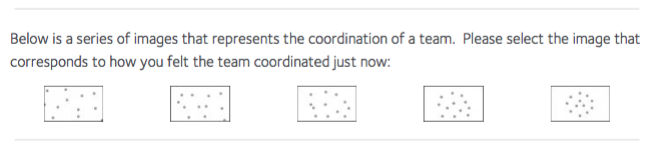
\includegraphics[width = \linewidth]{images/teamClickPictorial.png}
      \caption{Click Pictorial Scale}
      \label{fig:clickPictorial}
    \end{figure}


\myparagraph{\label{app8:bondingPre}Social Bonding}

  \begin{description}
    \item [Emotional Support] ``How emotionally supportive does the team feel?''
    \item [Shared Goal] ``How strong is the feeling that everyone is working towards a shared goal?''
    \item [Group Identification Verbal] A six-item scale designed to measure an individual's personal identification with the stereotypical features of the in-group  \citep{Mael1992}.  All 6 items were measured using a 5-point Likert scale.
          \begin{enumerate}
            \item When someone critises my team, it feels like a personal insult
            \item I am very interested in what others think about my team
            \item When I talk about my team, I usually say ``we'' rather than ``they''
            \item This team's successes are my successes
            \item When someone praises my team, it feels like a personal compliment
            \item If a story in the media criticises my team, I would feel embarrassed
          \end{enumerate}

  \item [Identity Fusion Verbal] A seven-item scale designed to measure an individual's ``feeling of oneness with the group'' \citep{Swann2009}.  Identity Fusion is differentiated from Group Identification in its ability to account for an individual's felt, emotional and personal agentic associations with being a member of the target in-group \citep{Swann2012a}.  All 7 items were measured using a 5-point Likert scale.
    \begin{enumerate}
      \item I am one with my team
      \item I feel immersed in my team
      \item I have a deep emotional bond with my team
      \item My team is me
      \item I’ll do for my team more than any of the other team members would do
      \item I am strong because of my team
      \item I make my team strong
    \end{enumerate}
  \item [Identity Fusion Pictorial] A visual scale designed to measure Identity Fusion to the target in-group \citep{Swann2009}. The pictorial scale depicts two circles, one smaller circle to denote the individual, and one larger circle to denote the group, progressively moving closer to each other such that the most ``fused'' option depicts the smaller circle encased by the larger circle. The scale offers a total of five options to chose from, see Figure ~\ref{fig:fusionPictorialGroup}.  A total of three pictorial scales were included, each with different target in-groups: team, family, and country (China).
  \item [Fusion Pictorial Rank] Athletes were asked to rank their fusion to team, family, and country \citep{Whitehouse2014}.  ``Thinking about these relationships [to team, family, and country] please rank them below in order of which you feel most connected to. 1 for most connected, 3 for least connected.''
  \end{description}


  \begin{figure}[htbp]
    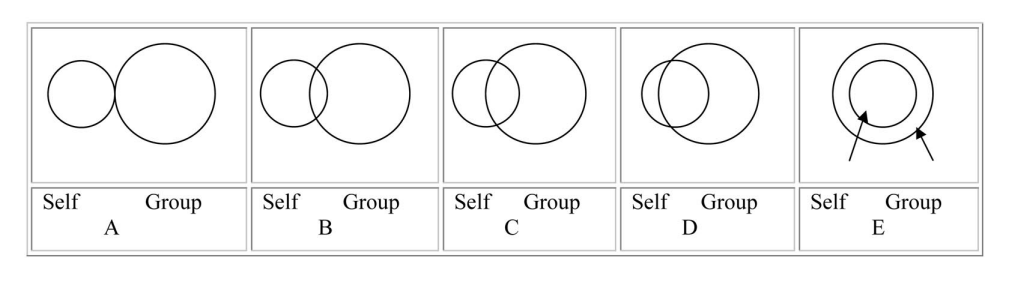
\includegraphics[width=\linewidth]{images/Identity_Fusion_Pictorial_Scale.png}
    \caption{Identity Fusion Pictorial Scale}
    \label{fig:fusionPictorialGroup}
  \end{figure}


\myparagraph{\label{app8:technicalCompetence}Subjective and Objective measures of technical competence}
Athletes were asked about their individual technical competence: ``Rate your individual ability in rugby, relative to: 1) Other teammates currently in your team, 2) Other current professional Chinese rugby players, 3) Professional rugby players form other countries.'' (Items were measured with a zero-centred 100 point scale, -50 - ``Extremely weak'', 0 - ``Average'', 50 - ``Extremely strong'').  Athletes were also asked about perceived competence of their team relative to other Chinese provincial teams: ``Rate your team's overall ability, relative to other teams in China'' (100 point scale, -50 - ``Extremely weak'', 0 - ``Average'', 50 - ``Extremely strong'').  In addition, athletes were asked if their perception of recent performance influences their 1) mood and 2) confidence regarding future performance (All these items were measured with a zero-centred 100 point scale, -50 - ``Extremely weak'', 0 - ``Average'', 50 - ``Extremely strong'').

Athletes were asked to report rugby-related attributes that would provide a more objective indicator of technical competence. These measures included: 1) rugby training age (number of years of experience training for rugby, to the nearest number of years), 2) the number of years spent training with the provincial teams (to the nearest year) , 5) whether the athlete is a usual member of the provincial program's starting team or the reserves.


\myparagraph{\label{app8:TIPI}Ten Item Personality Index}
Athletes were asked to indicate on a 7-point Likert scale the extent to which they agreed with 10 pairs of adjectives as appropriate descriptions of their personality. For example: ``I see myself as: dependable, self-disciplined'' (Response: 1 - ``Disagree strongly'', 2 - ``Disagree moderately'',  3 - ``Disagree a little'', 4 - ``Neither agree nor disagree'', 5 - ``Agree a little'', 6 - ``Agree moderately'', 7 - ``Agree strongly''). In the TIPI, two survey items corresponded to each of the big-five personality types, as follows:

\begin{description}
\item [Extraversion:] 1. Extraverted, enthusiastic; 6. Reserved, quiet (Reversed scale)
\item [Agreeableness:] 2. Critical, quarrelsome (Reversed); 7. Sympathetic, warm
\item [Conscientiousness:] 3. Dependable, self-disciplined; 8. Disorganised, careless (Reversed)
\item [Emotional Stability:] 4. Anxious, easily upset (Reversed); 9. Calm, emotionally stable.
\item [Openness to Experiences:] 5. Open to new experiences, complex; 10.Conventional, uncreative (Reversed)
\end{description}


\myparagraph{\label{app8:teamDisciplinePre}Team Discipline}
Athletes were asked about their feelings regarding their team's commitment to aspects of team discipline over the past month (punctuality to training and team meetings, observing bed times and curfews, attendance at meals, general team conduct) (100 point scale for each item, 0 - ``Extremely poor'', 100 - ``Extremely strong'')).

\myparagraph{Injury Status \label{app8:injuryStatus}}
Athletes responded to a question item asking about their injury status: ``Currently, are you physically able participate in a game?'' (100-point scale (0 = ``Unable to play'', 100 = ``Completely fit to play'').

\myparagraph{Identification Variables\label{app8:IDVariables}}
In addition to the items mentioned in the main text, Athletes also reported their date of birth, team affiliation, usual playing position (forward or back), contract and athlete status.






\subsubsection{\label{app8:surveyMid}Mid-Tournament Survey Items}

\myparagraph{\label{app8:performMid}Performance Items}
\begin{description}
\item [Individual Performance Expectations]``Overall, how do you feel about your individual performance in this game?''
\item [Team Performance Expectations] ``Overall, how do you feel about your team's performance in this game?''
\end{description}
Both items used a zero-centred continuous scale, -50 = ``much worse than expected'', 0 =  ``As expected'', 50 =  ``much better than expected''.

\myparagraph{\label{app8:exertionMid}Arousal, Exertion, and Fatigue}
Following each mid-Tournament survey and in the post-Tournament survey, Athletes were asked to report on various components of physical and mental fatigue, exertion, and injury. Athletes were asked about their mood (``How are you feeling now after the tournament?'') and responded by choosing a point on a 10-point scale between three pairs of emotions (``Not aroused / highly aroused'',  ``Depressed/Relaxed'' and  ``Nervous/Excited'').  Athletes were also asked about feelings of fatigue ``How fatigued do you feel as a result of the game/tournament?'', perceived physical exertion (Borg RPE scale, \citep{Borg1990} and perceived mental exertion using two 15-point scales \citep[see][ ]{Noakes2012a}.  Athletes were also asked to indicate their injury status on a 100-point scale (0 = ``Unable to play'', 100 = ``Completely fit to play'').




\subsubsection{\label{app8:surveyPost}Post-Tournament Survey Items}
The post-Tournament survey repeated the mid-Tournament items, asking:
\begin{description}
\item [Individual Performance Expectations] ``Overall, how do you feel about your individual performance during the tournament?''
\item [Team Performance Expectations]``Overall, how do you feel about your team's performance during the tournament?''
\end{description}




\subsubsection{\label{app8:objectivePerformance}Objective Performance Measures}

\begin{description}
\item [Final Rank:] A rank was given to each team based on performance in their respective competition (men's and women's). These rank scores were then reversed for the purposes of statistical analysis (1st place in men's Tournament (8 teams) = 8, 2nd place = 7, and so on)
\item [Total Wins - Losses:] A team's total number of losses was subtracted from its total number of wins.  Thus, more successful teams overall had a higher score.
\item [Total Minutes:] Total number of minutes played throughout the Tournament by each individual athlete
\item [Total Points:] Total number of points scored throughout the Tournament by each individual athlete
\item [Starting Team Average] An average measure indicating likelihood of an athlete being selected in the starting team. Each Athlete was awarded 1 point for each game he or she started in the starting team; reserve squad athletes were awarded zero for each game. Each athlete's total was divided by the total number of games that they participated in during the Tournament, including games in which they didn't take the field, to produce an average score for the Tournament.
\end{description}





\section{Results}


\subsection{Descriptive Statistics}

\subsubsection{\label{app8:descriptivesPre}Pre-Tournament Data Descriptives}

\begin{table}[htpb]\caption{Summary Statistics: post-Tournament Technical Competence (objective and subjective)}
\begin{center}
\begin{small} 
\begin{tabular}
{l
r
r
r
r
r
r
r
}

\multicolumn{
7
}{l}{

}
\cr 
 \hline 
Variable  &  
n  & 
mean  & 
sd  & 
min  & 
max  & 
skew  & 
krtss \cr 

 \hline 

Years In Team   &  120  &   3.17  &   2.12  &    0  &   7  &   0.29  &  -1.25 \cr 

Training Age   &  120  &   4.40  &   2.35  &    0  &  13  &   0.47  &   0.66 \cr 

Starting Team Average   &  172  &   0.61  &   0.36  &    0  &   1  &  -0.43  &  -1.32 \cr 

Age   &  121  &  21.67  &   3.26  &   16  &  32  &   0.52  &  -0.27 \cr 

Ability Teammates   &  120  &  19.45  &  20.14  &  -40  &  50  &  -0.31  &  -0.56 \cr 

Ability Chinese Pros   &  120  &  15.78  &  19.59  &  -35  &  50  &  -0.18  &  -0.65 \cr 

Ability International   &  120  &  18.46  &  26.19  &  -44  &  50  &  -0.48  &  -0.77 \cr 

Team Ability China   &  120  &  22.48  &  22.90  &  -40  &  50  &  -0.64  &  -0.58 \cr 

 \hline 
\end{tabular}
\end{small}
\end{center}
\label{tab:1competenceDescriptives}
\end{table} 




Table ~\ref{tab:1competenceDescriptives} displays the variables relevant to an Athlete's technical competence.  These variables were collected in the pre-Tournament survey, and as such the number of observations per variable is generally 120, except for ``Starting Team Average,'' which was generated from the objective performance data provided by CRFA following the Tournament.  The average number of years in the team was over three years, and the average training age for Athletes was 4.4 years.  In terms of subjective confidence, means for each variable were well above the mid-point of the scale, suggesting that Athletes were on average quite positive about their own ability compared to other athletes (their teammates, other Chinese professionals, International professionals).

\subsubsection{mid-Tournament Data}



\subsubsection{post-Tournament Data}


% Table created by stargazer v.5.2 by Marek Hlavac, Harvard University. E-mail: hlavac at fas.harvard.edu
% Date and time: Mon, Jun 26, 2017 - 09:48:21
\begin{table}[!htbp] \centering 
  \caption{Overall Tournament Performance Summary Statistics} 
  \label{tab:performanceOverallSummary} 
\scriptsize 
\begin{tabular}{@{\extracolsep{5pt}} ccccccccc} 
\\[-1.8ex]\hline 
\hline \\[-1.8ex] 
time & teamPerf & tP.sd & indPerf & iP.sd & teamPerfExp & tPE.sd & indPerfExp & iP.sd.1 \\ 
\hline \\[-1.8ex] 
pre-Tournament & $71.11$ & $21.87$ & $68.92$ & $21.32$ & $$ & $$ & $$ & $$ \\ 
day1 & $$ & $$ & $$ & $$ & $54.43$ & $30.63$ & $39.43$ & $27.25$ \\ 
day2 & $$ & $$ & $$ & $$ & $53.19$ & $32.98$ & $40.92$ & $27.93$ \\ 
post-Tournament & $$ & $$ & $$ & $$ & $64.36$ & $23.61$ & $56.36$ & $23.47$ \\ 
\hline \\[-1.8ex] 
\end{tabular} 
\end{table} 


% Table created by stargazer v.5.2 by Marek Hlavac, Harvard University. E-mail: hlavac at fas.harvard.edu
% Date and time: Mon, Jun 26, 2017 - 09:21:29
\begin{table}[!htbp] \centering 
  \caption{Team Click Overall Tournament Summary Statistics} 
  \label{tab:clickOverallSummary} 
\scriptsize 
\begin{tabular}{@{\extracolsep{5pt}} ccccccc} 
\\[-1.8ex]\hline 
\hline \\[-1.8ex] 
time & unspUnd & uU.sd & genAt & gA.sd & clickPic & cP.sd \\ 
\hline \\[-1.8ex] 
pre-Tournament & $71.58$ & $20.77$ & $75.51$ & $23.27$ & $3.87$ & $1.24$ \\ 
day1 & $55.92$ & $26.88$ & $65.74$ & $31.95$ & $3.46$ & $1.49$ \\ 
day2 & $55.30$ & $29.43$ & $64.32$ & $33.39$ & $3.33$ & $1.70$ \\ 
post-Tournament & $72.72$ & $19.95$ & $78.45$ & $21.34$ & $3.93$ & $1.04$ \\ 
\hline \\[-1.8ex] 
\end{tabular} 
\end{table} 


% Table created by stargazer v.5.2 by Marek Hlavac, Harvard University. E-mail: hlavac at fas.harvard.edu
% Date and time: Mon, Jun 26, 2017 - 09:22:14
\begin{table}[!htbp] \centering 
  \caption{Social Bonding Overall Tournament Summary Statistics} 
  \label{tab:bondingOverallSummary} 
\scriptsize 
\begin{tabular}{@{\extracolsep{5pt}} ccccccc} 
\\[-1.8ex]\hline 
\hline \\[-1.8ex] 
time & emoSup & eS.sd & sharedGoal & sG.sd & fusionPic & fP.sd \\ 
\hline \\[-1.8ex] 
pre-Tournament & $70.12$ & $26.21$ & $77.66$ & $24.28$ & $4.26$ & $1.25$ \\ 
day1 & $67.29$ & $30.56$ & $76.34$ & $30.50$ & $4.06$ & $1.47$ \\ 
day2 & $67.53$ & $32.55$ & $71.42$ & $35.47$ & $3.85$ & $1.69$ \\ 
post-Tournament & $79.67$ & $18.84$ & $86$ & $15.56$ & $4.33$ & $1.19$ \\ 
\hline \\[-1.8ex] 
\end{tabular} 
\end{table} 

%
% Table created by stargazer v.5.2 by Marek Hlavac, Harvard University. E-mail: hlavac at fas.harvard.edu
% Date and time: Mon, Jun 26, 2017 - 09:23:43
\begin{table}[!htbp] \centering 
  \caption{Fatigue Overall Tournament Summary Statistics} 
  \label{tab:fatigueOverallSummary} 
\scriptsize 
\begin{tabular}{@{\extracolsep{5pt}} ccccccccc} 
\\[-1.8ex]\hline 
\hline \\[-1.8ex] 
time & fat & f.sd & prpe & p.sd & mental & m.sd & inj.mu & inj.sd \\ 
\hline \\[-1.8ex] 
pre-Tournament & $$ & $$ & $$ & $$ & $$ & $$ & $18.73$ & $23.36$ \\ 
day1 & $50.14$ & $28.80$ & $12.45$ & $4.52$ & $4.09$ & $2.83$ & $29.91$ & $33.15$ \\ 
day2 & $53.65$ & $31.03$ & $12.60$ & $5.53$ & $4.13$ & $3.17$ & $37.14$ & $37.66$ \\ 
post-Tournament & $69.27$ & $21.24$ & $14.97$ & $2.66$ & $6.08$ & $2.47$ & $23.86$ & $26.91$ \\ 
\hline \\[-1.8ex] 
\end{tabular} 
\end{table} 



\begin{table}[htpb]\caption{Summary Statistics: post-Tournament Performance (individual and team)}
\begin{center}
\begin{small} 
\begin{tabular}
{l
r
r
r
r
r
r
r
}

\multicolumn{
7
}{l}{

}
\cr 
 \hline 
Variable  &  
{n} & 
{mean} & 
{sd} & 
{min} & 
{max} & 
{skew} & 
{krtss}\cr 

 \hline 

indPerformance7   &  118  &  56.36  &  23.47  &  0  &  100  &  -0.35  &  -0.08 \cr 

passingTech7   &  118  &  58.41  &  24.25  &  0  &  100  &  -0.79  &   0.05 \cr 

supportAttack7   &  118  &  62.62  &  22.70  &  0  &  100  &  -0.98  &   0.64 \cr 

indDefense7   &  118  &  57.64  &  23.57  &  0  &  100  &  -0.55  &  -0.11 \cr 

effectContact7   &  118  &  62.15  &  24.81  &  0  &  100  &  -0.97  &   0.40 \cr 

decisionAttack7   &  118  &  61.22  &  21.43  &  0  &  100  &  -0.72  &   0.37 \cr 

teamPerformance7   &  118  &  64.36  &  23.61  &  0  &  100  &  -0.52  &  -0.30 \cr 

teamDefense7   &  118  &  62.42  &  22.50  &  0  &  100  &  -0.52  &  -0.52 \cr 

teamAttack7   &  118  &  65.33  &  20.26  &  0  &  100  &  -0.53  &  -0.23 \cr 

teamSupportPlay7   &  118  &  65.75  &  19.72  &  0  &  100  &  -0.76  &   0.57 \cr 

teamCommunication7   &  118  &  65.25  &  21.26  &  0  &  100  &  -0.65  &   0.27 \cr 

 \hline 
\end{tabular}
\end{small}
\end{center}
\label{tab:2performancePostDescriptives}
\end{table} 



\begin{table}[htpb]\caption{Summary Statistics: post-Tournament Team Click}
\begin{center}
\begin{small} 
\begin{tabular}
{l
r
r
r
r
r
r
r
}

\multicolumn{
7
}{l}{

}
\cr 
 \hline 
Variable  &  
{n} & 
{mean} & 
{sd} & 
{min} & 
{max} & 
{skew} & 
{krtss}\cr 

 \hline 

unspokenUnderstanding7   &  118  &  72.72  &  19.95  &  0  &  100  &  -1.38  &  2.13 \cr 

generalAtmosphere7   &  118  &  78.45  &  21.34  &  0  &  100  &  -1.51  &  2.82 \cr 

clickPictorial7   &  118  &   3.93  &   1.04  &  1  &    5  &  -0.78  &  0.00 \cr 

reliabilityOfOthers7   &  118  &  68.00  &  23.09  &  0  &  100  &  -1.33  &  1.75 \cr 

reliabilityForOthers7   &  118  &  63.45  &  25.80  &  0  &  100  &  -1.06  &  0.51 \cr 

abilityExtended7   &  118  &  72.25  &  19.27  &  0  &  100  &  -1.13  &  2.03 \cr 

 \hline 
\end{tabular}
\end{small}
\end{center}
\label{tab:3clickPostDescriptives}
\end{table} 



\begin{table}[htpb]\caption{Summary Statistics: post-Tournament Social Bonding}
\begin{center}
\begin{small} 
\begin{tabular}
{l
r
r
r
r
r
r
r
}

\multicolumn{
7
}{l}{

}
\cr 
 \hline 
Variable  &  
{n} & 
{mean} & 
{sd} & 
{min} & 
{max} & 
{skew} & 
{krtss}\cr 

 \hline 

emotionalSupport7   &  118  &  79.67  &  18.84  &   0.00  &  100  &  -1.74  &  4.37 \cr 

sharedGoal7   &  118  &  86.00  &  15.56  &  29.00  &  100  &  -1.38  &  2.24 \cr 

groupId7   &  118  &   4.29  &   0.67  &   1.50  &    5  &  -1.18  &  1.66 \cr 

fusionVerbal7   &  118  &   4.00  &   0.71  &   1.43  &    5  &  -0.86  &  0.99 \cr 

fusionPictorialTeam7   &  118  &   4.33  &   1.19  &   0.00  &    5  &  -2.45  &  6.07 \cr 

fusionPictorialFamily7   &  118  &   4.51  &   0.96  &   0.00  &    5  &  -2.30  &  5.62 \cr 

fusionPictorialCountry7   &  118  &   4.03  &   1.39  &   0.00  &    5  &  -1.59  &  1.84 \cr 

 \hline 
\end{tabular}
\end{small}
\end{center}
\label{tab:4bondingPostDescriptives}
\end{table} 




\begin{table}[htpb]\caption{Summary Statistics: post-Tournament measures of fatigue}
\begin{center}
\begin{small} 
\begin{tabular}
{l
r
r
r
r
r
r
r
}

\multicolumn{
7
}{l}{

}
\cr 
 \hline 
Variable  &  
n  & 
mean  & 
sd  & 
min  & 
max  & 
skew  & 
krtss \cr 

 \hline 

Fatigue   &  118  &  69.27  &  21.24  &   0  &  100  &  -1.13  &  1.40 \cr 

RPE(physical)   &  118  &  14.97  &   2.66  &   6  &   20  &  -0.80  &  0.49 \cr 

RPE(mental)   &  118  &   6.08  &   2.47  &  -4  &   10  &  -1.13  &  1.82 \cr 

injuryRev7   &  118  &  23.86  &  26.91  &   0  &  100  &   1.19  &  0.60 \cr 

 \hline 
\end{tabular}
\end{small}
\end{center}
\label{tab:5fatiguePostDescriptives}
\end{table} 





\begin{table}[htpb]\caption{Summary Statistics: Objective Tournament Performance}
\begin{center}
\begin{small} 
\begin{tabular}
{l
r
r
r
r
r
r
r
}

\multicolumn{
7
}{l}{

}
\cr 
 \hline 
Variable  &  
n  & 
mean  & 
sd  & 
min  & 
max  & 
skew  & 
krtss \cr 

 \hline 

Final Rank   &  174  &   4.83  &   2.15  &   1  &   8  &  -0.09  &  -1.17 \cr 

Wins - Losses   &  172  &   0.32  &   2.94  &  -6  &   6  &  -0.17  &  -0.25 \cr 

Total Ind Points   &  172  &   8.45  &  11.41  &   0  &  69  &   2.34  &   7.23 \cr 

Total Ind Minutes   &  172  &  44.01  &  20.65  &   1  &  81  &  -0.38  &  -0.89 \cr 

Starting Team Avg   &  172  &   0.61  &   0.36  &   0  &   1  &  -0.43  &  -1.32 \cr 

 \hline 
\end{tabular}
\end{small}
\end{center}
\label{tab:6objectiveTournamentDescriptives}
\end{table} 





Table ~\ref{tab:2performancePostDescriptives} shows that the central tendency for individual and team performance measures was well above the mid-point of the scale, with team performance items slightly higher that individual performance items.  This negatively skewed central tendency in survey responses was more pronounced for variables relating to team click (as Table ~\ref{tab:3clickPostDescriptives} indicates), with the central tendency for each variable ranging between 65 and 78 (100-point scale, SD range = 19-27). The exception to this was the 5-point Team Click Pictorial Scale, the average for which was 3.93 (out of 5, SD = 1.04).  All six items relating to team click had a pronounced negative skew.  As Table ~\ref{tab:4bondingPostDescriptives} demonstrates, the trend for bonding was even higher; central tendencies for Emotional Support and Shared Goal were 79.67 (SD = 18.84) and 86 (SD = 15.56) respectively.  Group Identification Verbal Scale, and Identity Fusion Verbal and Pictorial Scales (5-point Likert) also had a high negatively skewed distribution, with central tendencies between 4 (Identity Fusion Verbal, SD = .71) and 4.51 (Identity Fusion Family, SD = 0.96).
In addition to these main variables of interest, the central tendency of distributions of responses related to arousal, exertion, and fatigue were also well above the mid-point of their respective scales (see Table ~\ref{tab:5fatiguePostDescriptives}).  Table ~\ref{tab:6objectiveTournamentDescriptives} displays athlete objective performance in the Tournament. Athletes played an average of 44 minutes of rugby during the Tournament (just under four full games each), and each Athlete scored an average of 8.45 points, which amounts to between one and two tries each, or a number of try drop-kick conversions (worth two points each).





%<<surveyMeasureSummaryTable, fig.cap =''>>=
%#create all columns:
%Items <- c(IndPerformance, GroupPerformance, TeamPerformance, GroupClick, TeamClick, GroupBonding, TeamBonding, Arousal, Exertion)
%Baseline <- c("*","","*","","*","","*","","")
%Pre <- c("*","*","","*","","*","","*","")
%Post <- c("*","*","","*","*","*","*","*","*")

%surveyMeasureSummary <- data.frame(Variable, Baseline, Pre, Post, stringsAsFactors = FALSE)

%summaryTable <- xtable(surveyMeasureSummary)
%align(summaryTable) <- xalign(summaryTable)
%summaryTable
%@















\begin{enumerate}
  \item A focussed analysis of the \textbf{post-Tournament} survey responses
  \item An analysis of \textit{changes} in variables between \textbf{pre- and post-Tournament} responses
  \item Analysis of the relationship between team performance, team click, and social bonding in survey data over the \textbf{entire Tournament}. \textit{Note that these data are still under analysis and will not be presented for assessment here.}
\end{enumerate}




\subsubsection{Pre-post Tournament differences in variables of interest}
Pre- and Post-Tournament measures of variables of interest are displayed in tables below.  Three out of five variables measuring athletes' perceived success in components of individual performance appeared to drop from Pre- to Post-Tournament (see Table ~\ref{tab:indPerformancePrePostSummary}).  Paired samples t-tests revealed significant negative mean differences between Pre- and Post-Tournament measures of passing technique ($M = -7.48 (-13.17, -1.80)$, $t(98)= -2.61,, p = .01$), support play ($M = -7.32 (-12.18, -2.47)$, $t(98)= -2.99,, p = .003$), and decision making in attack ($M = -5.19 ( -9.73, -.65)$, $t(98)= -2.27,, p = .03$), while individual defence ($M = -3.42 (-9.01, 2.16)$, $t(98)= -1.22,, p = .23$), and effectiveness in contact ($M = -4.51 (-10.25, 1.24)$, $t(98)= -1.56,, p = .12$) did not decrease significantly between Pre- and Post-Tournament measures.

By contrast, all four variables measuring team success in components of joint action did not differ significantly between Pre- and Post-Tournament measurements (see Table ~\ref{tab:teamPerformancePrePostSummary} for results).  Similarly, variables measuring team click also did not vary significantly.  These results suggest that athlete perceptions of team joint action success and team click on average remained stable throughout the Tournament.  Perceptions of success in individual component performance, by contrast, decreased significantly, indicating that following the Tournament athletes were on average more critical of their performance.

In terms of Social Bonding, both feelings of emotional support and feelings of Common Goal with the team differed significantly between Pre- and Post-Tournament measurements (see Table ~\ref{tab:bondingPrePostSummary}). Both measures increased significantly in the Post-Tournament measure (emotional support: $M = 9.30 (4.16, 14.45)$, $t(98)= 3.59,, p = .0005$; Common Goal $M = 7.12 (3.06, 11.19)$, $t(98)= 3.48,, p = .0007$).  All other variables did not vary significantly from Pre-Tournament measures, except for the pictorial measure of fusion to \textit{family}, which increased significantly, $M = .33(.03, .64)$, $t(98)= 2.18, p = .03$.  Bonding variables for which measures were 5-point Likert may have suffered from ceiling effects: the mean and median of each Fusion Pictorial scale was $> 4$.  In general, it appeared that bonding to the team (and to one measure of Family) increased when measured following the Tournament.

In addition, variables measuring feelings of exertion and fatigue also varied significantly between Pre- and Post-Tournament measurements.  Fatigue ($M = 21.61 (15.02 28.20)$, $t(116)= 6.49,, p < .0001$), physical perceived exertion ($M = 2.84 (1.89, 3.79)$, $t(116)= 5.93, p < .0001$), and mental perceived exertion ($M = 2.84 (1.89, 3.79)$, $t(116)= 5.93, p < .0001$) all increased significantly from the point of first measurement immediately following the 2nd game on Day 1 of the Tournament (see Table ~\ref{tab:fatiguePrePostSummary}).  Injury status Post-Tournament did not differ significantly from Pre-Tournament measures when tested using a paired-samples t-test, although the overall group mean difference between Pre- and Post-Tournament injury did show marginally significant signs of increasing, $M = 2.84 (-10.63, .59)$, $t(98)= 1.78, p = .08$.
These results indicate that on average, athletes felt higher levels of exertion and fatigue after the Tournament, than they did before or after the first game of the Tournament. This is to be expected, given the intensity of the rugby sevens Tournament format, and it confirms for the strenuous nature of the activity of the present study.





\clearpage


\newgeometry{margin=0.5cm} % modify this if you need even more space
\begin{landscape}

% Table created by stargazer v.5.2 by Marek Hlavac, Harvard University. E-mail: hlavac at fas.harvard.edu
% Date and time: Sun, Jun 25, 2017 - 22:44:09
\begin{table}[!htbp] \centering 
  \caption{Individual Performance change pre-post Tournament} 
  \label{tab:indPerformancePrePostSummary} 
\footnotesize 
\begin{tabular}{@{\extracolsep{5pt}} cccccccccc} 
\\[-1.8ex]\hline 
\hline \\[-1.8ex] 
 & Variable & Mean.pre & SD.pre & Mean.post & SD.post & MeanDiffernece & MeanPairedDifference & t-test & p-value \\ 
\hline \\[-1.8ex] 
1 & passingTechnique & $65.74$ & $24.94$ & $58.41$ & $24.25$ & $$-$7.33$ & $$-$7.48$ & $$-$2.61$ & $0.01$ \\ 
2 & supportPlay & $69.54$ & $23.23$ & $62.62$ & $22.70$ & $$-$6.92$ & $$-$7.32$ & $$-$2.99$ & $0.003$ \\ 
3 & individualDefense & $59.22$ & $26.64$ & $57.64$ & $23.57$ & $$-$1.57$ & $$-$3.42$ & $$-$1.22$ & $0.23$ \\ 
4 & effectivenessContact & $65.66$ & $24.85$ & $62.15$ & $24.81$ & $$-$3.51$ & $$-$4.51$ & $$-$1.56$ & $0.12$ \\ 
5 & decisionMakingAttack & $65.48$ & $23.80$ & $61.22$ & $21.43$ & $$-$4.26$ & $$-$5.19$ & $$-$2.27$ & $0.03$ \\ 
\hline \\[-1.8ex] 
\end{tabular} 
\end{table} 


% Table created by stargazer v.5.2 by Marek Hlavac, Harvard University. E-mail: hlavac at fas.harvard.edu
% Date and time: Sun, Jun 25, 2017 - 22:47:06
\begin{table}[!htbp] \centering 
  \caption{Team Performance change pre-post Tournament} 
  \label{tab:teamPerformancePrePostSummary} 
\footnotesize 
\begin{tabular}{@{\extracolsep{5pt}} cccccccccc} 
\\[-1.8ex]\hline 
\hline \\[-1.8ex] 
 & Variable & Mean.pre & SD.pre & Mean.post & SD.post & MeanDiffernece & MeanPairedDifference & t-test & p-value \\ 
\hline \\[-1.8ex] 
1 & teamDefense & $65.06$ & $22.85$ & $62.42$ & $22.50$ & $$-$2.63$ & $$-$4.92$ & $$-$1.57$ & $0.12$ \\ 
2 & teamAttack & $66.01$ & $24.95$ & $65.33$ & $20.26$ & $$-$0.68$ & $$-$1.59$ & $$-$0.55$ & $0.58$ \\ 
3 & teamSupportPlay & $64.36$ & $23.53$ & $65.75$ & $19.72$ & $1.40$ & $0.90$ & $0.35$ & $0.73$ \\ 
4 & teamCommunication & $62.37$ & $24.21$ & $65.25$ & $21.26$ & $2.89$ & $$-$0.07$ & $$-$0.03$ & $0.98$ \\ 
\hline \\[-1.8ex] 
\end{tabular} 
\end{table} 


% Table created by stargazer v.5.2 by Marek Hlavac, Harvard University. E-mail: hlavac at fas.harvard.edu
% Date and time: Sat, Jun 03, 2017 - 15:44:29
\begin{table}[!htbp] \centering 
  \caption{click change pre-post Tournament} 
  \label{} 
\footnotesize 
\begin{tabular}{@{\extracolsep{5pt}} cccccccccc} 
\\[-1.8ex]\hline 
\hline \\[-1.8ex] 
 & Variable & Mean.pre & SD.pre & Mean.post & SD.post & MeanDiffernece & MeanPairedDifference & t-test & p-value \\ 
\hline \\[-1.8ex] 
1 & unspokenUnderstanding & $71.58$ & $20.77$ & $72.72$ & $19.95$ & $1.14$ & $1.33$ & $0.58$ & $0.56$ \\ 
2 & generalAtmosphere & $75.51$ & $23.27$ & $78.45$ & $21.34$ & $2.94$ & $1.05$ & $0.47$ & $0.64$ \\ 
3 & clickPictorial & $3.87$ & $1.24$ & $3.93$ & $1.04$ & $0.07$ & $0.03$ & $0.21$ & $0.84$ \\ 
4 & reliabilityOfOthers & $67.43$ & $28.01$ & $68$ & $23.09$ & $0.57$ & $1.21$ & $0.40$ & $0.69$ \\ 
5 & reliabilityForOthers & $62.38$ & $25.40$ & $63.45$ & $25.80$ & $1.07$ & $1.06$ & $0.38$ & $0.70$ \\ 
6 & abilityExtended & $70.45$ & $25.83$ & $72.25$ & $19.27$ & $1.80$ & $1.43$ & $0.53$ & $0.60$ \\ 
\hline \\[-1.8ex] 
\end{tabular} 
\end{table} 


% Table created by stargazer v.5.2 by Marek Hlavac, Harvard University. E-mail: hlavac at fas.harvard.edu
% Date and time: Sun, Jun 25, 2017 - 22:51:01
\begin{table}[!htbp] \centering 
  \caption{bonding change pre-post Tournament} 
  \label{tab:bondingPrePostSummary} 
\footnotesize 
\begin{tabular}{@{\extracolsep{5pt}} cccccccccc} 
\\[-1.8ex]\hline 
\hline \\[-1.8ex] 
 & Variable & Mean.pre & SD.pre & Mean.post & SD.post & MeanDiffernece & MeanPairedDifference & t-test & p-value \\ 
\hline \\[-1.8ex] 
1 & emotionalSupport & $70.12$ & $26.21$ & $79.67$ & $18.84$ & $9.55$ & $9.30$ & $3.59$ & $0.001$ \\ 
2 & sharedGoal & $77.66$ & $24.28$ & $86$ & $15.56$ & $8.34$ & $7.12$ & $3.48$ & $0.001$ \\ 
3 & groupId & $4.34$ & $0.78$ & $4.29$ & $0.67$ & $$-$0.04$ & $0.06$ & $0.78$ & $0.44$ \\ 
4 & fusionVerbal & $4.03$ & $0.74$ & $4.00$ & $0.71$ & $$-$0.03$ & $0$ & $0$ & $1$ \\ 
5 & fusionPictorialTeam & $4.26$ & $1.25$ & $4.33$ & $1.19$ & $0.07$ & $0.04$ & $0.30$ & $0.77$ \\ 
6 & fusionPictorialCountry & $4.01$ & $1.58$ & $4.03$ & $1.39$ & $0.02$ & $$-$0.04$ & $$-$0.22$ & $0.83$ \\ 
7 & fusionPictorialFamily & $4.10$ & $1.50$ & $4.51$ & $0.96$ & $0.41$ & $0.33$ & $2.18$ & $0.03$ \\ 
8 & rankTeam & $1.49$ & $0.79$ & $1.61$ & $0.81$ & $0.12$ & $0.09$ & $1.15$ & $0.25$ \\ 
9 & rankCountry & $1.92$ & $1.06$ & $1.93$ & $1.03$ & $$ & $$-$0.04$ & $$-$0.44$ & $0.66$ \\ 
10 & rankFamily & $1.41$ & $0.88$ & $1.42$ & $0.86$ & $0.01$ & $0$ & $0$ & $1$ \\ 
\hline \\[-1.8ex] 
\end{tabular} 
\end{table} 


% Table created by stargazer v.5.2 by Marek Hlavac, Harvard University. E-mail: hlavac at fas.harvard.edu
% Date and time: Sun, Jun 25, 2017 - 23:08:36
\begin{table}[!htbp] \centering 
  \caption{Fatigue change pre-post Tournament} 
  \label{fatiguePrePostSummary} 
\footnotesize 
\begin{tabular}{@{\extracolsep{5pt}} cccccccccc} 
\\[-1.8ex]\hline 
\hline \\[-1.8ex] 
 & Variable & Mean.pre & SD.pre & Mean.post & SD.post & MeanDiffernece & MeanPairedDifference & t-test & p-value \\ 
\hline \\[-1.8ex] 
1 & fatigue & $50.14$ & $28.80$ & $69.27$ & $21.24$ & $19.13$ & $21.61$ & $6.49$ & $0$ \\ 
2 & prpe & $12.45$ & $4.52$ & $14.97$ & $2.66$ & $2.52$ & $2.84$ & $5.93$ & $0.0000$ \\ 
3 & mental & $4.09$ & $2.83$ & $6.08$ & $2.47$ & $1.99$ & $2.30$ & $6.85$ & $0$ \\ 
4 & injury & $81.28$ & $23.36$ & $76.14$ & $26.91$ & $$-$5.13$ & $5.02$ & $1.78$ & $0.08$ \\ 
\hline \\[-1.8ex] 
\end{tabular} 
\end{table} 


\end{landscape}
\restoregeometry

\bigskip





















Although the ICC value for Social Bonding was relatively low, a group-wise means difference test (computed using a linear regression model) revealed significant team level differences in mean Social Bonding, $F(14, 103) = 1.84, p = .04, R^2 = .09$).


\section{\label{app8:stats}Statistical Method}

\subsection{\label{app8:EFA}Data Reduction using Exploratory Factor Analysis}
EFA is one of various available data reduction techniques, and is distinct from its main alternative, Principal Components Analysis (PCA), in that it is capable of modelling the latent dimensions of a collection of variables.\footnote{PCA is concerned only with establishing which components exist within the existing data and how a particular variable might contribute that component. To do this, PCA makes the assumption that all variance in a subset of variables is common variance, and therefore communality between all variables is equal to 1. From this assumption, the original data can be transposed into a linear model without the need for a communality-dependent estimated coefficient for each variable \citep{Widaman2007}. EFA examines all the pairwise relationships between individual variables and seeks to extract latent factors from the measured variables.  Squared Multiple Correlations (which are essentially multiple regressions in which each variable is predicted by all others) were used to calculate the common variance (communality) between each variable in an analysis (the communality value is much like an R-squared value from a multiple regression).
The square root of the communality score for each variable is then used as a coefficient that conditions the relationship between each variable and the underlying dimensions (factors) identifiable in the data. Also known as ``factor loadings,'' these coefficients become the parameters of linear model capable of estimating factor scores for each individual observation, which can be utilised in subsequent statistical analysis in place of single variable observations.

A final step in the EFA procedure is the process of ``rotation'', which is an optimisation technique designed to encourage each variable to load on as few factors as possible \citep{Rummel1988}. Rotation refers to a geometric conception of factor analysis, in which individual variables can be plotted in n-dimensional space according to their relationship to each dimension (factor). By rotating the axes of these dimensions, the distance of a given variable to that dimension can be reduced, which results in an increase in factor loading on one factor and (ideally) a decrease in factor loading on another uncorrelated variable. Orthogonal (or perpendicular) rotation of axes refers to axes, say X and Y, maintaining a 90-degree perpendicularity and rotating clockwise or anticlockwise, depending on the location of the variable clusters.
Orthogonal rotation thus enables optimisation of loadings for clusters of variables that are distant from each other in n-dimensional space. If correlation exists between clusters of variables, however, rotating axes obliquely (inwards towards each other) provides a more effective way of reducing the distance between clusters of variables and the latent dimensions that account for such clustering \citep{Osborne2015}. See Figure ~\ref{fig:orthogonalOblique} for a graphical  illustration of the difference between orthogonal and oblique rotation. Given that most variables of interest in the present study were correlated to some degree, I opted for an oblique rotation method \citep{Field2012}. EFAs were conducted using the factanal() function in the Stats package (Version 3.3.0) in R, using the ``promax'' (oblique) rotation method \citep{Gorsuch1983}. Factor scores were calculated as standardised z-scores: zero-centred, with a standard deviation of 1.

\begin{figure}[htbp]
  \begin{center}
    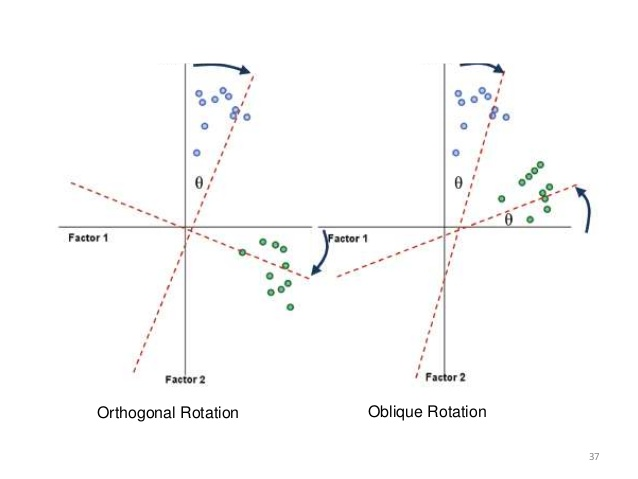
\includegraphics[width= \linewidth, scale = .5]{images/orthogonalObliqueRotationExample.jpg}
    \caption{Orthogonal and oblique rotation methods}
    \label{fig:orthogonalOblique}
  \end{center}
\end{figure}



\subsubsection{\label{app8:samplingAdequacy}Sampling adequacy measures: KMO and Bartlett's Test for Sphericity}

The KMO index provides a proportion measure of common variance to partial correlations among examined variables.  If the KMO index is high ($\approx$ 1), the EFA can act efficiently; if KMO is low ($\approx$ 0), the proposed EFA is not suitable for analysis.

Bartlett’s test of sphericity is used to test the null hypothesis that the correlation matrix is an identity matrix (i.e., a square matrix in which all the elements of the principal diagonal are equal to 1, and all other elements are 0s).

\subsubsection{\label{app8:reliabilityMeasures}Reliability measures: Cronbach's alpha and Guttman's lambda3}


\footnote{Cronbach's $\alpha$ is a function of the number of items in a test, the average covariance between item-pairs, and the variance of the total score \citep{Tabachnick2007}}








\subsection{Data Reduction Summary}


\subsubsection{post-Tournament Data Reduction}

\myparagraph{\label{app8:performanceDataReduction}Team and Individual Components of Performance}
Sampling adequacy measures indicated high suitability ($KMO = 0.83$, $\chi^2(36, N = 118) = 726.60$, $p < .0001$).  As expected, an EFA extracted two factors, with Individual performance measures loaded on one factor (proportion of variance = .34, $SS Loading = 3.09$), and team performance measures loading on a second factor (proportion of variance = .32, $SS Loading = 2.90$). $Guttman's \lambda =.93$ and $Cronbach's \alpha = .90$ indicated that the data reduction was appropriate.





\newpage
\newgeometry{margin=0.5cm} % modify this if you need even more space
\begin{landscape}


% Table created by stargazer v.5.2.2 by Marek Hlavac, Harvard University. E-mail: hlavac at fas.harvard.edu
% Date and time: Mon, Aug 27, 2018 - 18:51:00
\begin{table}[!htbp] \centering 
  \caption{Correlation Matrix: post-Tournament Technical Competence} 
  \label{tab:1competenceCorr} 
\scriptsize 
\begin{tabular}{@{\extracolsep{5pt}} ccccccccc} 
\\[-1.8ex]\hline 
\hline \\[-1.8ex] 
 & Years In Team & Training Age & Starting Team Average & Age & Ability Teammates & Ability Chinese Pros & Ability International & Team Ability China \\ 
\hline \\[-1.8ex] 
Years In Team & $1$ & $0.510$ & $$-$0.044$ & $0.569$ & $0.076$ & $0.102$ & $0.099$ & $0.261$ \\ 
Training Age & $0.510$ & $1$ & $0.0004$ & $0.697$ & $0.095$ & $0.183$ & $0.201$ & $0.190$ \\ 
Starting Team Average & $$-$0.044$ & $0.0004$ & $1$ & $$-$0.040$ & $0.203$ & $0.099$ & $0.044$ & $0.144$ \\ 
Age & $0.569$ & $0.697$ & $$-$0.040$ & $1$ & $0.132$ & $0.089$ & $0.154$ & $0.212$ \\ 
Ability Teammates & $0.076$ & $0.095$ & $0.203$ & $0.132$ & $1$ & $0.428$ & $0.383$ & $0.454$ \\ 
Ability Chinese Pros & $0.102$ & $0.183$ & $0.099$ & $0.089$ & $0.428$ & $1$ & $0.702$ & $0.273$ \\ 
Ability International & $0.099$ & $0.201$ & $0.044$ & $0.154$ & $0.383$ & $0.702$ & $1$ & $0.212$ \\ 
Team Ability China & $0.261$ & $0.190$ & $0.144$ & $0.212$ & $0.454$ & $0.273$ & $0.212$ & $1$ \\ 
\hline \\[-1.8ex] 
\end{tabular} 
\end{table} 


% Table created by stargazer v.5.2 by Marek Hlavac, Harvard University. E-mail: hlavac at fas.harvard.edu
% Date and time: Sun, Jun 25, 2017 - 21:08:16
\begin{table}[!htbp] \centering 
  \caption{Correlation Matrix: post-Tournament Team Performance} 
  \label{tab:22teamPerformancePostCorr} 
\footnotesize 
\begin{tabular}{@{\extracolsep{5pt}} ccccc} 
\\[-1.8ex]\hline 
\hline \\[-1.8ex] 
 & Team Defence & Team Attack & Team Support Play & Team Onfield Communication \\ 
\hline \\[-1.8ex] 
Team Defence & $1$ & $0.834$ & $0.643$ & $0.721$ \\ 
Team Attack & $0.834$ & $1$ & $0.740$ & $0.713$ \\ 
Team Support Play & $0.643$ & $0.740$ & $1$ & $0.715$ \\ 
Team Onfield Communication & $0.721$ & $0.713$ & $0.715$ & $1$ \\ 
\hline \\[-1.8ex] 
\end{tabular} 
\end{table} 


% Table created by stargazer v.5.2 by Marek Hlavac, Harvard University. E-mail: hlavac at fas.harvard.edu
% Date and time: Sun, Jun 25, 2017 - 21:07:58
\begin{table}[!htbp] \centering 
  \caption{Correlation Matrix: Individual Performance} 
  \label{tab:21indPerformancePostCorr} 
\footnotesize 
\begin{tabular}{@{\extracolsep{5pt}} cccccc} 
\\[-1.8ex]\hline 
\hline \\[-1.8ex] 
 & Passing Tech & Support In Attack & Ind Defence & Effectiveness In Contact & Decision Making Attack \\ 
\hline \\[-1.8ex] 
Passing Tech & $1$ & $0.658$ & $0.510$ & $0.508$ & $0.607$ \\ 
Support In Attack & $0.658$ & $1$ & $0.658$ & $0.641$ & $0.734$ \\ 
Ind Defence & $0.510$ & $0.658$ & $1$ & $0.590$ & $0.525$ \\ 
Effectiveness In Contact & $0.508$ & $0.641$ & $0.590$ & $1$ & $0.713$ \\ 
Decision Making Attack & $0.607$ & $0.734$ & $0.525$ & $0.713$ & $1$ \\ 
\hline \\[-1.8ex] 
\end{tabular} 
\end{table} 


% Table created by stargazer v.5.2.2 by Marek Hlavac, Harvard University. E-mail: hlavac at fas.harvard.edu
% Date and time: Mon, Aug 27, 2018 - 18:51:00
\begin{table}[!htbp] \centering 
  \caption{Correlation Matrix: post-Tournament Team Click} 
  \label{} 
\footnotesize 
\begin{tabular}{@{\extracolsep{5pt}} ccccccc} 
\\[-1.8ex]\hline 
\hline \\[-1.8ex] 
 & unspokenUnderstanding7 & generalAtmosphere7 & clickPictorial7 & reliabilityOfOthers7 & reliabilityForOthers7 & abilityExtended7 \\ 
\hline \\[-1.8ex] 
unspokenUnderstanding7 & $1$ & $0.626$ & $0.508$ & $0.275$ & $0.230$ & $0.375$ \\ 
generalAtmosphere7 & $0.626$ & $1$ & $0.385$ & $0.301$ & $0.276$ & $0.265$ \\ 
clickPictorial7 & $0.508$ & $0.385$ & $1$ & $0.282$ & $0.021$ & $0.213$ \\ 
reliabilityOfOthers7 & $0.275$ & $0.301$ & $0.282$ & $1$ & $0.276$ & $0.544$ \\ 
reliabilityForOthers7 & $0.230$ & $0.276$ & $0.021$ & $0.276$ & $1$ & $0.375$ \\ 
abilityExtended7 & $0.375$ & $0.265$ & $0.213$ & $0.544$ & $0.375$ & $1$ \\ 
\hline \\[-1.8ex] 
\end{tabular} 
\end{table} 


\clearpage

% Table created by stargazer v.5.2 by Marek Hlavac, Harvard University. E-mail: hlavac at fas.harvard.edu
% Date and time: Tue, May 30, 2017 - 09:19:43
\begin{table}[!htbp] \centering 
  \caption{Correlation Matrix: post-Tournament Social Bonding} 
  \label{} 
\footnotesize 
\begin{tabular}{@{\extracolsep{5pt}} cccccc} 
\\[-1.8ex]\hline 
\hline \\[-1.8ex] 
 & emotionalSupport & sharedGoal & groupIdentification & identityFusionVerbal & identityFusionPictorialTeam \\ 
\hline \\[-1.8ex] 
emotionalSupport & $1$ & $0.619$ & $0.079$ & $0.331$ & $0.349$ \\ 
sharedGoal & $0.619$ & $1$ & $0.061$ & $0.246$ & $0.395$ \\ 
groupIdentification & $0.079$ & $0.061$ & $1$ & $0.358$ & $0.081$ \\ 
identityFusionVerbal & $0.331$ & $0.246$ & $0.358$ & $1$ & $0.220$ \\ 
identityFusionPictorialTeam & $0.349$ & $0.395$ & $0.081$ & $0.220$ & $1$ \\ 
\hline \\[-1.8ex] 
\end{tabular} 
\end{table} 


% Table created by stargazer v.5.2 by Marek Hlavac, Harvard University. E-mail: hlavac at fas.harvard.edu
% Date and time: Sat, Jun 03, 2017 - 22:22:24
\begin{table}[!htbp] \centering 
  \caption{Correlation Matrix: post-Tournament Fatigue} 
  \label{} 
\footnotesize 
\begin{tabular}{@{\extracolsep{5pt}} ccccc} 
\\[-1.8ex]\hline 
\hline \\[-1.8ex] 
 & fatigue & RPE(physical) & RPE(mental) & injuryRev7 \\ 
\hline \\[-1.8ex] 
fatigue & $1$ & $0.665$ & $0.510$ & $0.090$ \\ 
RPE(physical) & $0.665$ & $1$ & $0.523$ & $0.009$ \\ 
RPE(mental) & $0.510$ & $0.523$ & $1$ & $$-$0.040$ \\ 
injuryRev7 & $0.090$ & $0.009$ & $$-$0.040$ & $1$ \\ 
\hline \\[-1.8ex] 
\end{tabular} 
\end{table} 


% Table created by stargazer v.5.2 by Marek Hlavac, Harvard University. E-mail: hlavac at fas.harvard.edu
% Date and time: Tue, May 30, 2017 - 09:19:44
\begin{table}[!htbp] \centering 
  \caption{Tournament Performance Correlation Matrix} 
  \label{} 
\footnotesize 
\begin{tabular}{@{\extracolsep{5pt}} cccccc} 
\\[-1.8ex]\hline 
\hline \\[-1.8ex] 
 & finalRank & totalWins - totalLosses & totalIndPoints & totalMinutesPlayed & startingTeamAvg \\ 
\hline \\[-1.8ex] 
finalRank & $1$ & $0.901$ & $0.381$ & $0.062$ & $0.055$ \\ 
totalWins - totalLosses & $0.901$ & $1$ & $0.428$ & $0.129$ & $0.089$ \\ 
totalIndPoints & $0.381$ & $0.428$ & $1$ & $0.404$ & $0.067$ \\ 
totalMinutesPlayed & $0.062$ & $0.129$ & $0.404$ & $1$ & $$-$0.038$ \\ 
startingTeamAvg & $0.055$ & $0.089$ & $0.067$ & $$-$0.038$ & $1$ \\ 
\hline \\[-1.8ex] 
\end{tabular} 
\end{table} 


\clearpage
\begin{table}[htpb]\caption{Summary Statistics: post-Tournament Factors}
\begin{center}
\begin{scriptsize} 
\begin{tabular}
{l
r
r
r
r
r
r
r
}

\multicolumn{
7
}{l}{

}
\cr 
 \hline 
Variable  &  
n  & 
mean  & 
sd  & 
min  & 
max  & 
skew  & 
krtss \cr 

 \hline 

objCompetence   &  120  &   0.00  &   0.95  &  -1.99  &    2.91  &   0.45  &  -0.23 \cr 

subjCompetence   &  120  &   0.00  &   0.96  &  -2.58  &    1.79  &  -0.16  &  -0.66 \cr 

indPerformExp   &  118  &  56.36  &  23.47  &   0.00  &  100.00  &  -0.35  &  -0.08 \cr 

indPerformSuccess   &  118  &   0.00  &   0.95  &  -2.96  &    1.70  &  -0.85  &   0.60 \cr 

teamPerformanceExpect   &  118  &  64.36  &  23.61  &   0.00  &  100.00  &  -0.52  &  -0.30 \cr 

jointActionSuccess   &  118  &   0.00  &   0.96  &  -3.28  &    1.79  &  -0.49  &  -0.01 \cr 

teamClick   &  118  &   0.00  &   0.90  &  -3.06  &    1.42  &  -1.01  &   1.03 \cr 

socialBonding   &  118  &   0.00  &   0.89  &  -3.08  &    1.08  &  -1.38  &   2.00 \cr 

fatigue   &  118  &   0.00  &   0.91  &  -3.40  &    1.67  &  -1.03  &   1.56 \cr 

 \hline 
\end{tabular}
\end{scriptsize}
\end{center}
\label{tab:postTournamentFactorDescriptives}
\end{table} 




% Table created by stargazer v.5.2.2 by Marek Hlavac, Harvard University. E-mail: hlavac at fas.harvard.edu
% Date and time: Mon, Aug 27, 2018 - 18:51:01
\begin{table}[!htbp] \centering 
  \caption{post-Tournament Factors Correlation Matrix} 
  \label{tab:postTournamentFactorCorr} 
\scriptsize 
\begin{tabular}{@{\extracolsep{5pt}} cccccccccc} 
\\[-1.8ex]\hline 
\hline \\[-1.8ex] 
 & objCompetence & subjCompetence & indPerformExp & indPerformSuccess & teamPerformanceExpect & jointActionSuccess & teamClick & socialBonding & fatigue \\ 
\hline \\[-1.8ex] 
objCompetence & $1$ & $$-$0.146$ & $0.065$ & $0.319$ & $$-$0.128$ & $$-$0.150$ & $0.011$ & $0.017$ & $0.084$ \\ 
subjCompetence & $$-$0.146$ & $1$ & $$-$0.086$ & $0.125$ & $$-$0.067$ & $0.044$ & $0.145$ & $0.195$ & $$-$0.045$ \\ 
indPerformExp & $0.065$ & $$-$0.086$ & $1$ & $0.411$ & $0.454$ & $0.285$ & $0.226$ & $0.180$ & $0.221$ \\ 
indPerformSuccess & $0.319$ & $0.125$ & $0.411$ & $1$ & $0.411$ & $0.490$ & $0.414$ & $0.273$ & $0.245$ \\ 
teamPerformanceExpect & $$-$0.128$ & $$-$0.067$ & $0.454$ & $0.411$ & $1$ & $0.709$ & $0.570$ & $0.314$ & $0.204$ \\ 
jointActionSuccess & $$-$0.150$ & $0.044$ & $0.285$ & $0.490$ & $0.709$ & $1$ & $0.686$ & $0.404$ & $0.202$ \\ 
teamClick & $0.011$ & $0.145$ & $0.226$ & $0.414$ & $0.570$ & $0.686$ & $1$ & $0.674$ & $0.271$ \\ 
socialBonding & $0.017$ & $0.195$ & $0.180$ & $0.273$ & $0.314$ & $0.404$ & $0.674$ & $1$ & $0.199$ \\ 
fatigue & $0.084$ & $$-$0.045$ & $0.221$ & $0.245$ & $0.204$ & $0.202$ & $0.271$ & $0.199$ & $1$ \\ 
\hline \\[-1.8ex] 
\end{tabular} 
\end{table} 



\end{landscape}
\restoregeometry


\subsection{\label{app:moderatorVarsEFA}Data Reduction for moderator variables}

\subsubsection{Fatigue}
\myparagraph{Post-Tournament}
Post-Tournament survey items relating to perceptions of fatigue and exertion were separately analysed for the purposes of data reduction.  Due to difficulty completing questions related to arousal in the online and in-person surveys, mood-related items were excluded from analysis.  In addition, it was clear from correlation values that injury status did not strongly correlate with other items relevant to fatigue and exertion, and was therefore also excluded from subsequent analysis (see Table ~\ref{tab:5fatiguePostCorr}).  The KMO index and Bartlett's test of sphericity indicated that the remaining subset of variables was appropriate for EFA, $KMO =  0.69$, $\chi^2(3, N = 118) = 111.93$, $p < .001$. EFA was performed on 3 remaining items (fatigue, physical perceived exertion, and mental perceived exertion), which imposed one factor labelled ``Fatigue Factor.''  The extracted factor explained 57.8\% of the overall variance (SS Loadings = 1.7, $Guttman's\lambda =.73$ and Cronbach's $\alpha = .80$).

\myparagraph{Pre- to post-Tournament}
Three survey items related to feelings of fatigue (mental, physical exertion, & fatigue - after the first game!)  were collected and subjected to EFA.
Correlations between variables were high (all $r's > .55$, $KMO = .7$, corrtest Bartlett: $\chi^2(3, N = 238) = 382.88$, $p < .001$).  As such, one factor (``Fatigue Pre Post'') was imposed, which explained 66.3\% of the overall variance (SS Loading = 1.99).  $Guttman's \lambda =.8$ and $Cronbach's \alpha = .85$ indicated that the data reduction was appropriate.
%  $\chi^2(0, N = 238) = 0 $, $p < .001$,

\myparagraph{Overall Tournament}
Fatigue items consisted of fatigue, physical exertion and mental exertion. Correlations between variables were high, indicating that imposing one factor was appropriate (all $r's > .62$, $KMO = 0.71$, $\chi^2(3, N = 440) =  677.37, p < .001$).  The factor imposed for fatigue, ``Fatigue Tournament,'' explained 69\% of the variance ($SS Loading = 2.07$) and $Guttman's \lambda =.82$ and Cronbach's $\alpha = .87$) indicated that the data reduction was reliable.



\subsubsection{Technical Competence}
\myparagraph{Post-Tournament}
Eight items relevant to technical competence were analysed in a correlation matrix to assess relatedness (see Table ~\ref{tab:1competenceCorr}). Medium correlations among measures of objective competence (three out of four items correlated at $> .3$) and among measures of subjective competence (all items except for team competence measure correlated at $> .3$) suggested that the data could be explained by two underlying factors. Team Ability Chinese Provinces was dropped from analysis due to low correlation with other competence variables, possibly because the item did not ask about an individual athlete’s competence (it referred instead to an athlete’s opinion of the competence of the team of which they were a member). An examination of the KMO measure of sampling adequacy ($KMO = .67$), and the Bartlett sphericity test indicated that two factors were adequate, $\chi^2(21, N = 120) = 239.71$, $p < .001$. \\

An EFA of technical competence variables revealed that items of interest loaded on two factors. The exception was the variable Starting Reserve, which failed to load on either factor, and was thus dropped from analysis. Measures of objective competence (Years Team, Training Age, and Age) loaded on the first factor, which was labelled ``Objective Competence'' because the measures were all objective markers of an athlete's competence.  Objective Competence explained 26.4\% of the total variance ($SS Loading = 1.85$). The remaining measures of subjective competence (Ability Teammates, Ability Chinese Pros, Ability International Pros) loaded on the remaining factor.  The second factor was labelled ``Subjective Competence'', due to the fact that all measures were the product of subjective self-report.  Subjective competence explained 23.8\% of the variance ($SS Loading = 1.67$). $Guttman's \lambda =.74$ and $Cronbach's \alpha = (.67)$ indicated that the data reduction was appropriate and reliable.

\myparagraph{Pre- to post-Tournament}
NA
\myparagraph{Overall Tournament}
NA

Summary statistics for the factors extracted from the post-Tournament data, and their correlations can be viewed in Appendix ~\ref{app8:tournamentSurvey} Section
 ~\ref{tab:postTournamentFactorDescriptives} and Table ~\ref{tab:postTournamentFactorCorr} respectively.


















\subsection{\label{app8:modelSelection}Model Selection}
Due to the dependencies in the data and missingness throughout, both traditional ANCOVA (analysis of co-variance) models linear mixed-effects regression models (LMER) are capable of incorporating both fixed and random effects into analysis of variance, however ANCOVA designs only allow the intercept (and not the regression slope) to vary according to level-2 variance, whereas LMER can model the variability of both intercept and slope across different groups of the predictor variable \citep{Field2012}. In addition, the ability of LMERs to deal with unbalanced designs (due to missing values) meant that a LMER was the most suitable modelling strategy for the present study



\section{Intra Class Correlation}

For team-level variance, a one-way random effects model was used, in which average within-team variance (Mean Square Within) of the response variable was divided by the average total variance of the response (Mean Square Total) \citep{Field2005a}.  Each athlete was member of one of 15 teams, which were considered to be sampled from a larger pool of potential teams, hence treated as random effects. The ICC was then interpreted as the percentage of total variance accounted for by group-level variables \citep{Wolak2012}.
To statistically account for the unbalanced design of the data, an adjusted sample-size coefficient (k) was calculated using an equation provided by \citep{Lessells1987}.  While there is no firm agreement on what is deemed meaningful within-group variance, an ICC ratio of $>.10-1.00$ with confidence intervals that do not include zero was considered an indication of non-random correlation of group-level residuals \citep{Bailey2011}. As Table ~\ref{tab:ICCsummaryTeam} and ~\ref{tab:ICCsummarySex} indicate, small to moderate team-level intra-class correlation of responses exist for factors of Objective Competence, Joint Action Success, Individual Performance Success, and Team Click.  ICCs for Social Bonding and Fatigue meanwhile were relatively low (all $r's <.1$). Sex-level ICCs were all relatively low, suggesting that sex-level variation could be ignored in subsequent inferential analyses.\\





\subsubsection{Intra-Class Correlation}
To assess the need for a statistical model capable of accounting for correlation of residuals, dependency in the data a was quantified using a ratio measure comparing within- and between-group variance, known as the intra-class correlation (ICC). Clustering in the data according to team or sex (the separate men's and women's Tournament) was considered.  In addition to an assessment of ICC values, mean differences in variables of interest were assessed. Owing to the large number of grouping variables (team = 15), pairwise t-tests were not an appropriate way to compute team-level mean differences. Missing values in the data also meant that a standard ANOVA test was also not optimal for multiple group mean comparisons.  Instead, linear regressions were used to approximate differences between group-level responses for post-Tournament survey responses.  Team was used as the predictor variable, and factors derived from performance, click, social bonding, and fatigue variables were used as the outcome variables.  Analyses revealed:

\begin{itemize}
  \item Significant team-level differences in perceptions of success in team component performance (Joint Action Success, $F(14, 103) = 5.63, p < .0001, R^2 = 0.36$) and perceptions of success in individual component performance (Individual Performance Success, $F(14, 103) = 3.23, p < .001, R^2 = 0.21$).
  \item Significant team-level differences in perceptions of overall team performance relative to prior expectations (Team Performance Expectations, $F(14, 103) = 5.96, p < .0001, R^2 = 0.37$), but not perceptions of overall individual performance relative to expectations (Individual Performance Expectations, $R^2 = 0.03 F(14, 103) = 1.24, p = .26$).
  \item Significant team-level differences in team click (Team Click, $F(14, 103) = 4.32, p < .0001, R^2 = 0.28$), significant team-level differences in social bonding $F(14, 103) = 1.84, p = .04, R^2 = 0.09$), but team-level variance of fatigue was not significantly different, (fatigue, $F(14, 103) = 1.46, p = .14, R^2 = 0.05$).
\end{itemize}

An analysis of sex-differences revealed:
\begin{itemize}
  \item Significant sex differences in perceptions of success in individual component performance (Individual Performance Success, $F(1, 116) = 8.03, p < .01, R^2 = 0.06$, men scored significantly higher in self-rated success in components of individual performance, $\beta = 0.48, SE = 0.1709, t(116) = 2.835 p < .01$), but not perceptions of team component performance (Joint Action Success, $F(1, 116) = .002, p = .97, R^2 = -0.009$), perceptions of overall team performance relative to prior expectations (Team Performance Expectations, $F(1, 116) = .09, p = .77, R^2 = -0.008$), or perceptions of overall individual performance relative to prior expectations (Individual Performance Expectations, $F(1, 116) = .05, p = .83, R^2 = -0.008 $).
  \item There were also no significant sex differences in team click (Team Click, $F(1, 116) = .43, p = .51, R^2 = -0.005$), or fatigue ($F(1, 116) = 2.35, p = .13, R^2 = .01 $), but there was a significant sex-difference in social bonding ($F(1, 116) 6.01, p = .02, R^2 = .04$).
\end{itemize}


% Table created by stargazer v.5.2 by Marek Hlavac, Harvard University. E-mail: hlavac at fas.harvard.edu
% Date and time: Sun, Jun 25, 2017 - 21:23:24
\begin{table}[!htbp] \centering 
  \caption{Intra-Class Correlations for post-Tournament Factors according to team} 
  \label{tab:ICCsummaryTeam} 
\small 
\begin{tabular}{@{\extracolsep{5pt}} cccccc} 
\\[-1.8ex]\hline 
\hline \\[-1.8ex] 
 & variable & ICC.team & LowerCI.team & UpperCI.team & k.adjusted.team \\ 
\hline \\[-1.8ex] 
1 & subjectiveCompetence & $0.011$ & $$-$0.057$ & $0.185$ & $8.476$ \\ 
2 & objectiveCompetence & $0.356$ & $0.175$ & $0.625$ & $8.476$ \\ 
3 & jointActionSuccess & $0.374$ & $0.190$ & $0.634$ & $7.768$ \\ 
4 & indPerformanceSuccess & $0.223$ & $0.074$ & $0.484$ & $7.768$ \\ 
5 & teamClick & $0.299$ & $0.130$ & $0.564$ & $7.768$ \\ 
6 & socialBonding & $0.098$ & $$-$0.010$ & $0.324$ & $7.768$ \\ 
7 & fatigue & $0.056$ & $$-$0.036$ & $0.261$ & $7.768$ \\ 
\hline \\[-1.8ex] 
\end{tabular} 
\end{table} 


% Table created by stargazer v.5.2 by Marek Hlavac, Harvard University. E-mail: hlavac at fas.harvard.edu
% Date and time: Sun, Jun 25, 2017 - 21:23:23
\begin{table}[!htbp] \centering 
  \caption{Intra-Class Correlations for post-Tournament Factors according to sex} 
  \label{tab:ICCsummarySex} 
\small 
\begin{tabular}{@{\extracolsep{5pt}} cccccc} 
\\[-1.8ex]\hline 
\hline \\[-1.8ex] 
 & variable & ICC.sex & LowerCI.sex & UpperCI.sex & k.adjusted.sex \\ 
\hline \\[-1.8ex] 
1 & subjectiveCompetence & $0.039$ & $$-$0.006$ & $0.983$ & $58.933$ \\ 
2 & objectiveCompetence & $0.092$ & $0.006$ & $0.992$ & $58.933$ \\ 
3 & jointActionSuccess & $$-$0.017$ & $$-$0.017$ & $0.014$ & $58.390$ \\ 
4 & indPerformanceSuccess & $0.108$ & $0.009$ & $0.993$ & $58.390$ \\ 
5 & teamClick & $$-$0.010$ & $$-$0.016$ & $0.881$ & $58.390$ \\ 
6 & socialBonding & $0.079$ & $0.003$ & $0.991$ & $58.390$ \\ 
7 & fatigue & $0.023$ & $$-$0.009$ & $0.976$ & $58.390$ \\ 
\hline \\[-1.8ex] 
\end{tabular} 
\end{table} 












\subsubsection{Mediation Analysis}
The hypothesised path of relationships outlined in predictions above (specifically: Joint Action Success $\rightarrow$ Team Click $\rightarrow$ Social Bonding) suggests the possibility that Joint Action Success exerts its influence on Social Bonding indirectly, via feelings of ``team click.''  A formal mediation analysis can be used to test the prediction that the relationship between perceptions of joint-action success and social bonding is mediated by feelings of team click, by analysing if and how an intervening variable is causally significant to the relationship between a predictor and an outcome variable. A variable is a mediator if it carries the influence of the predictor variable to an outcome variable, if it serves to explain (either partially or fully) the variance in the outcome variable attributable to the predictor. In the case of this analysis, do perceptions of joint-action success have an indirect effect on feelings of social bonding that is transmitted through feelings associated with team click?

\begin{figure}[htbp]
  \begin{center}
    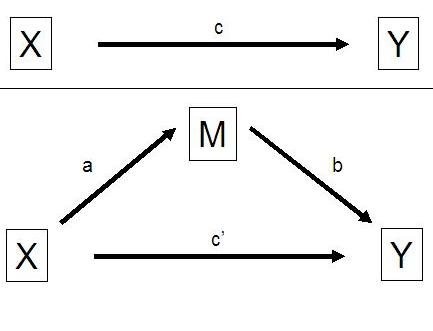
\includegraphics[scale = .5]{images/mediation_image.jpg}
    \caption{Mediation Analysis: direct and indirect effects}
    \label{fig:mediationAnalysis}
  \end{center}
\end{figure}

Mediation analysis works by testing the extent to which the variance in the outcome attributable to a predictor variable (the direct effect, or path ``c'': $Y_i \sim d_Y + cX_i + e_i$) can be explained \textit{indirectly} by the variance of two other relationships: that of the predictor variable and a third mediator (X $\rightarrow$ M, or path ``a'')  and M and the outcome variable (path ``b''), controlling for the direct relationship between X and Y (path ``'c'') (see Figure ~\ref{fig:mediationAnalysis}). The mediation model can thus be denoted by two equations:

\begin{equation}
  M_i \sim d_M + aX_i + e_Mi
\end{equation}

\begin{equation}
  Y_i \sim d_Y + bM_i + c'X_i +  + e_{Yi}
\end{equation}
\bigskip

When combined, these two equations enable the calculation of the ``indirect effect'' of the predictor on the outcome, by controlling for the relationship between the mediator's effect on the outcome variable as a function of its relationship to the predictor variable.  While the direct effect measures the extent to which the dependent variable changes when the independent variable increases by one unit and the mediator variable remains unaltered, the indirect effect measures the extent to which the dependent variable changes when the independent variable is held fixed and the mediator variable changes by the amount it would have changed had the independent variable increased by one unit \citep{Bauer2006}.

The multilevel structure of the data in this study, i.e. the clustering of residuals according to team affiliation, violates the independence assumption of mediation analysis. As such, traditional multiple linear regression and path analysis will produce biased tests of the effects in the mediation model \citep{Raudenbush2002}.
%(Hox, 2002; Kreft & de Leeuw, 1998; Raudenbush & Bryk, 2002).
A multilevel mediation analysis must therefore additionally take into account variance attributable to the random effects of the model (team, in this case), and in so doing capture heterogeneity of variance in the indirect effect due to the level 2 variable \citep{Tofighi2014}.  To do this, each coefficient in the model must be random (denoted by subscript ``j''), so that the value of the coefficient varies across Level 2 units (team): \\

\begin{equation}
  M_{ij} \sim d_{Mj} + a_jX_{ij} + e_{Mij}
\end{equation}

\begin{equation}
  Y_{ij} \sim d_{Yj} + b_jM_{ij} + 'c_jX_{ij} +  + e_{Yij}
\end{equation}
\bigskip

Linear mixed effects regression models are fitted according to these equations, and estimates of mediation effects can be computed from these model parameters.  Subsequent mediation analyses were conducted using the ``mediation'' function of the Causal Mediation Analysis Package (version 4.4.5) in R.






















\section{\label{app8:results}Results}
\subsection{\label{app8:modelRobustness}Model Robustness Checks}


\subsubsection{Prediction 1.a: Joint Action Success predicts Team Click}

BASIC XY RELATIONSHIP? (Post-Tournament Data)

In order to test the prediction that athlete perceptions of joint action are positively related to team click in the post-Tournament data, the following model was constructed:

\begin{equation}
  \begin{align*}
    Team Click =  & Joint Action Success\\
              & + Individual Performance Success \\
              & + Objective Competence + Subjective Competence\\
              & + TournamentPerformanceMeasures \\
  \end{align*}
\end{equation}
\bigskip


\begin{figure}[htbp]
    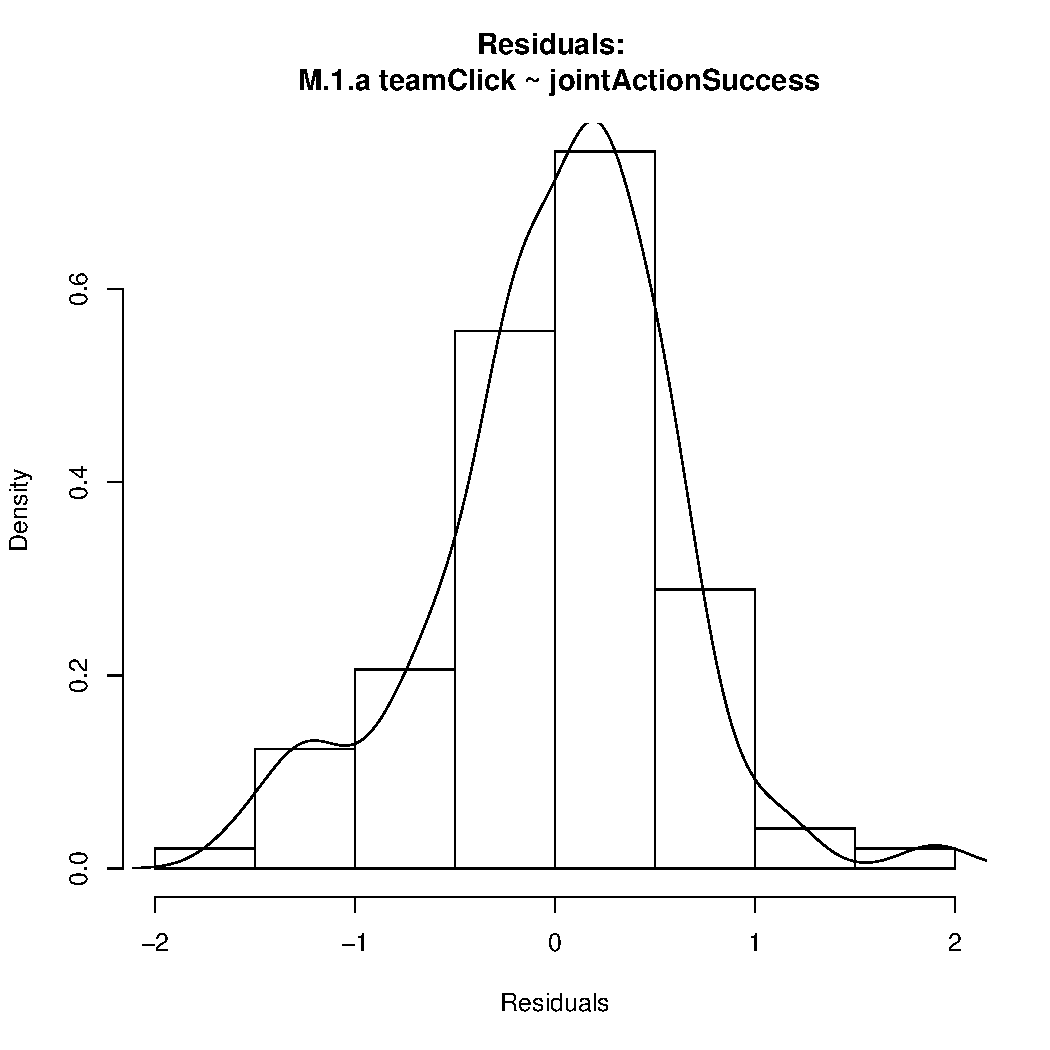
\includegraphics[scale =.4]{images/MLM1aHist.pdf}
    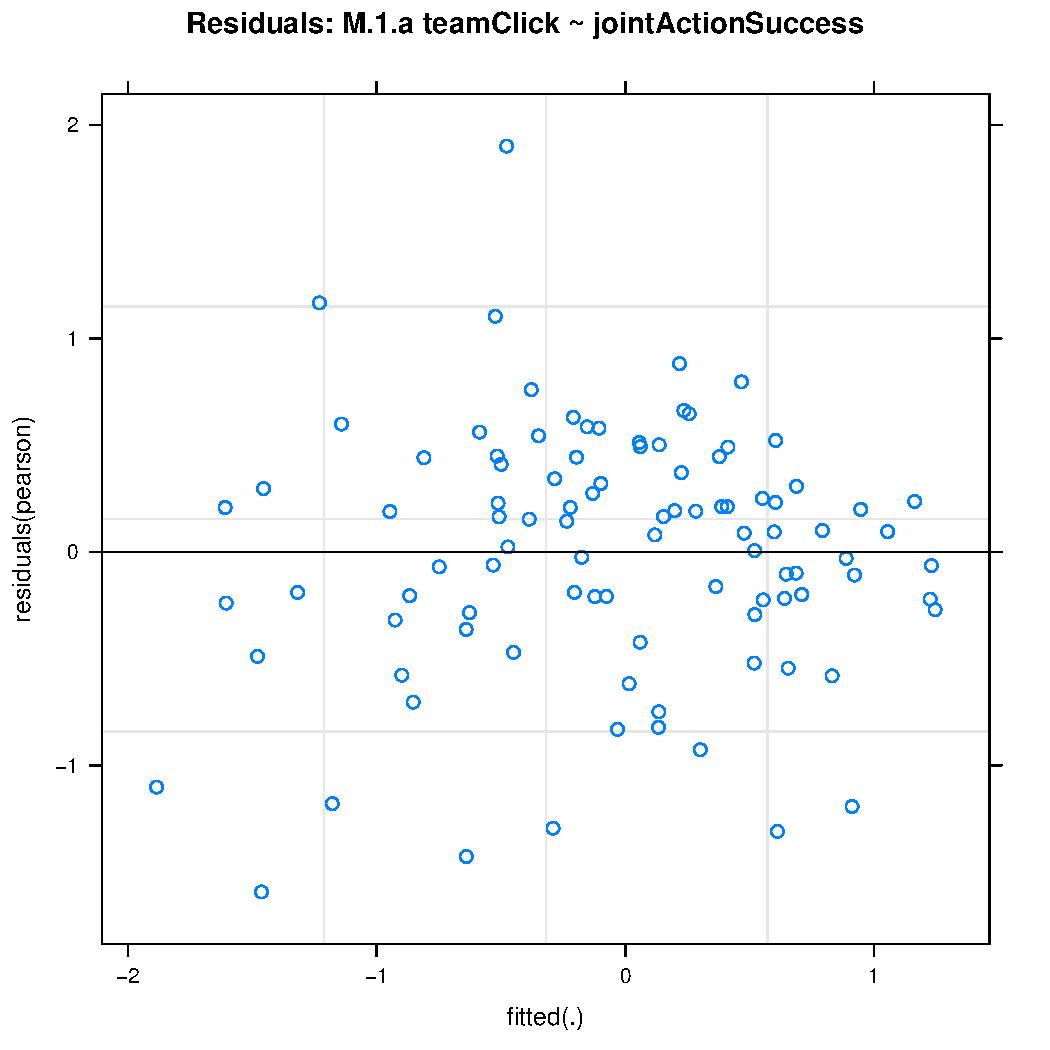
\includegraphics[scale =.4]{images/MLM1aScatter.pdf}
    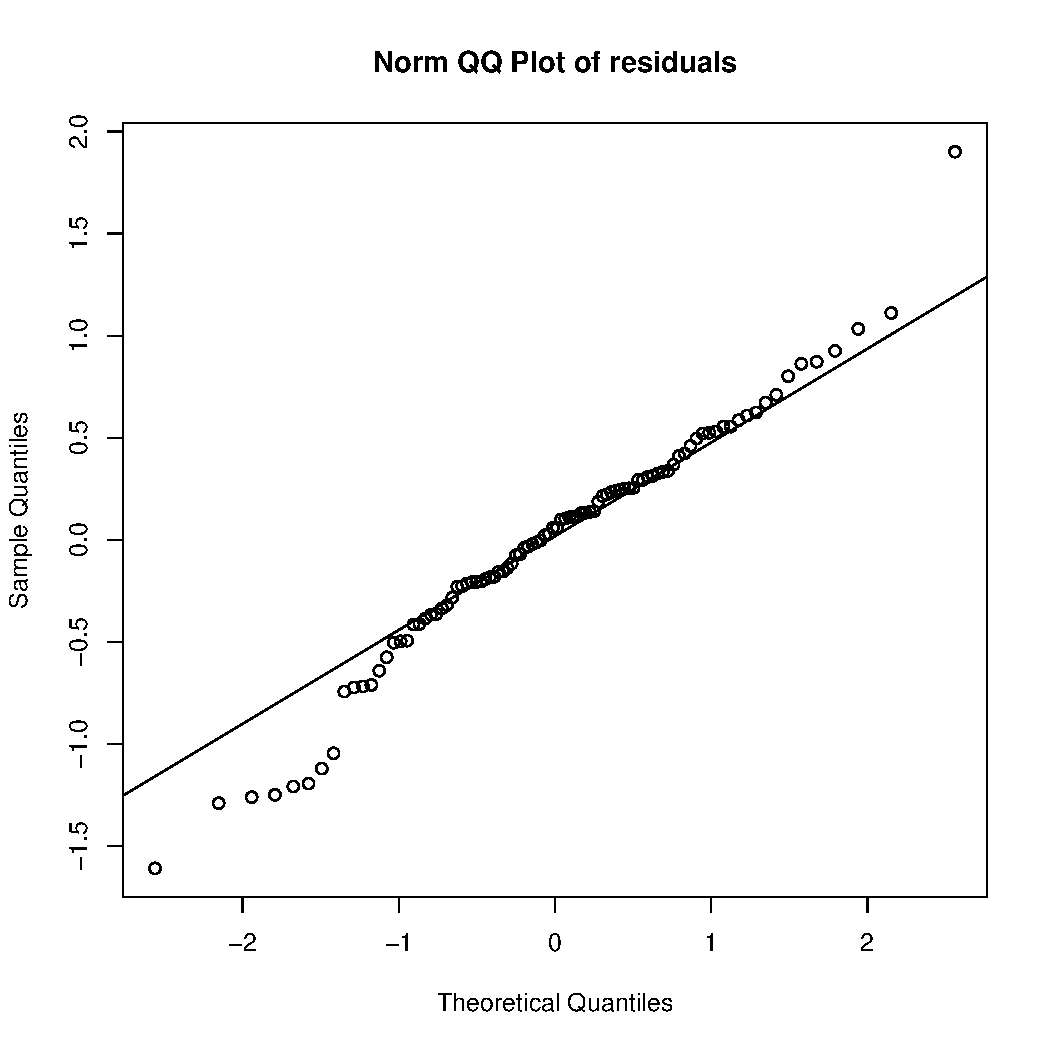
\includegraphics[scale =.4]{images/MLM1aQQPlot.pdf}
    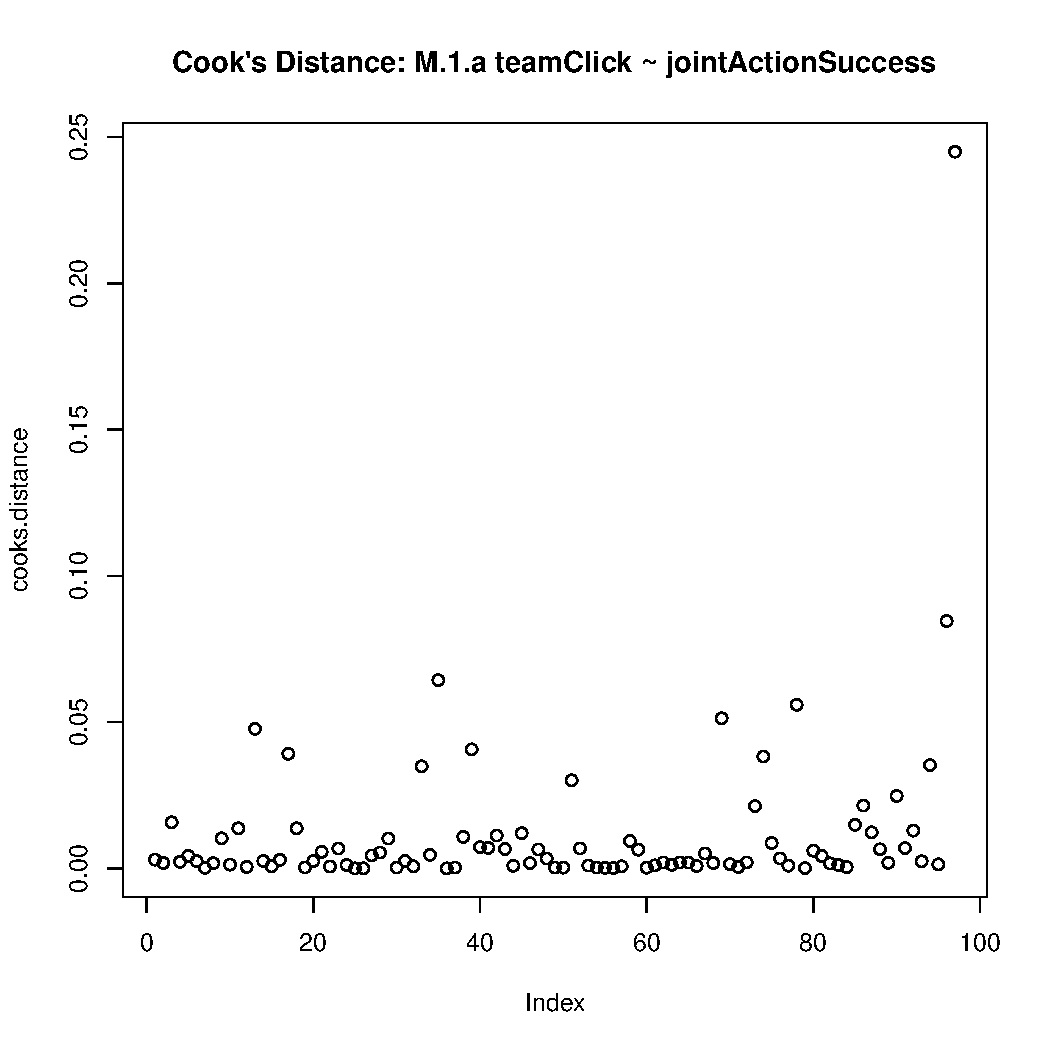
\includegraphics[scale =.4]{images/MLM1aCooksD.pdf}
    \caption{Model Assumptions: 1.a Joint Action Success Predicts Team Click}
    \label{fig:MLM1aAssumptions}
\end{figure}





\begin{figure}[htbp]
  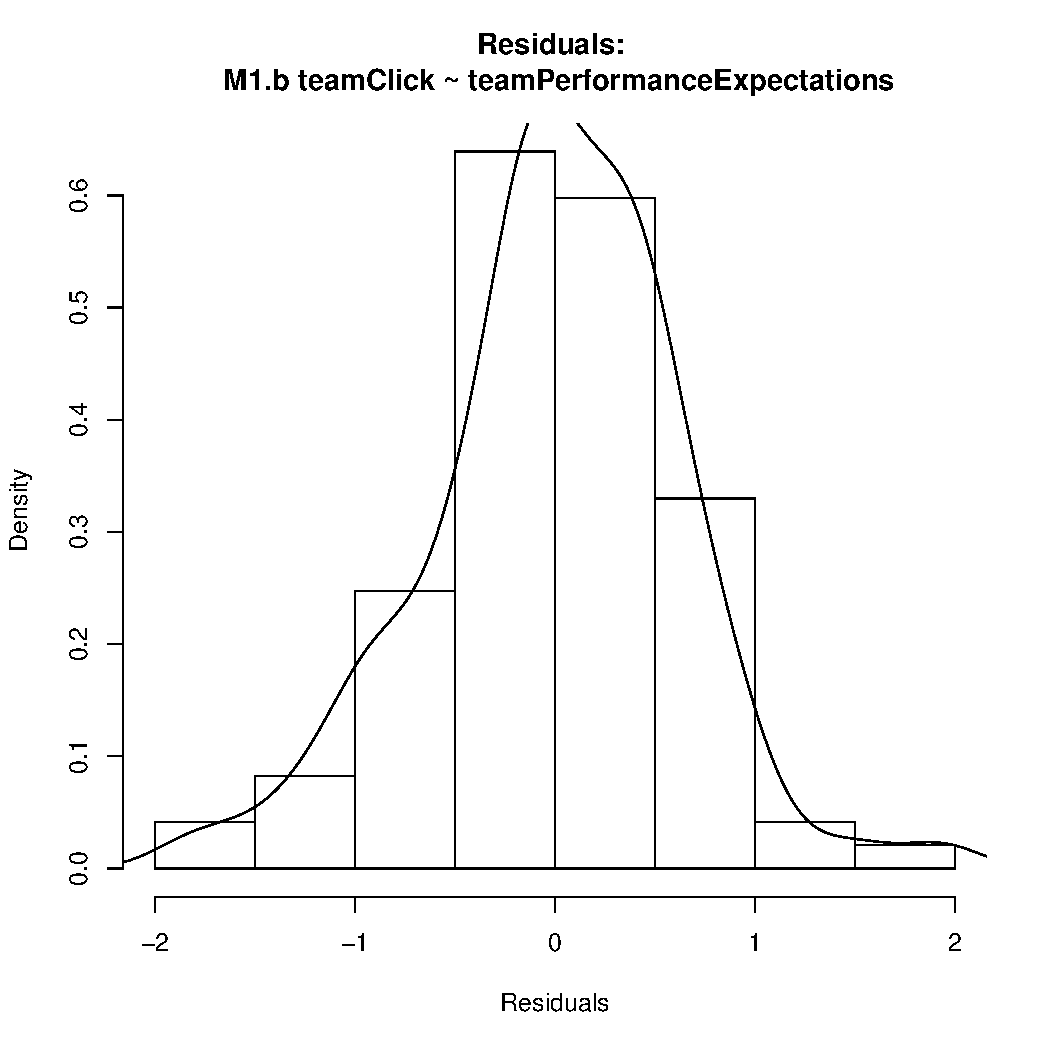
\includegraphics[scale =.4]{images/MLM1bHist.pdf}
  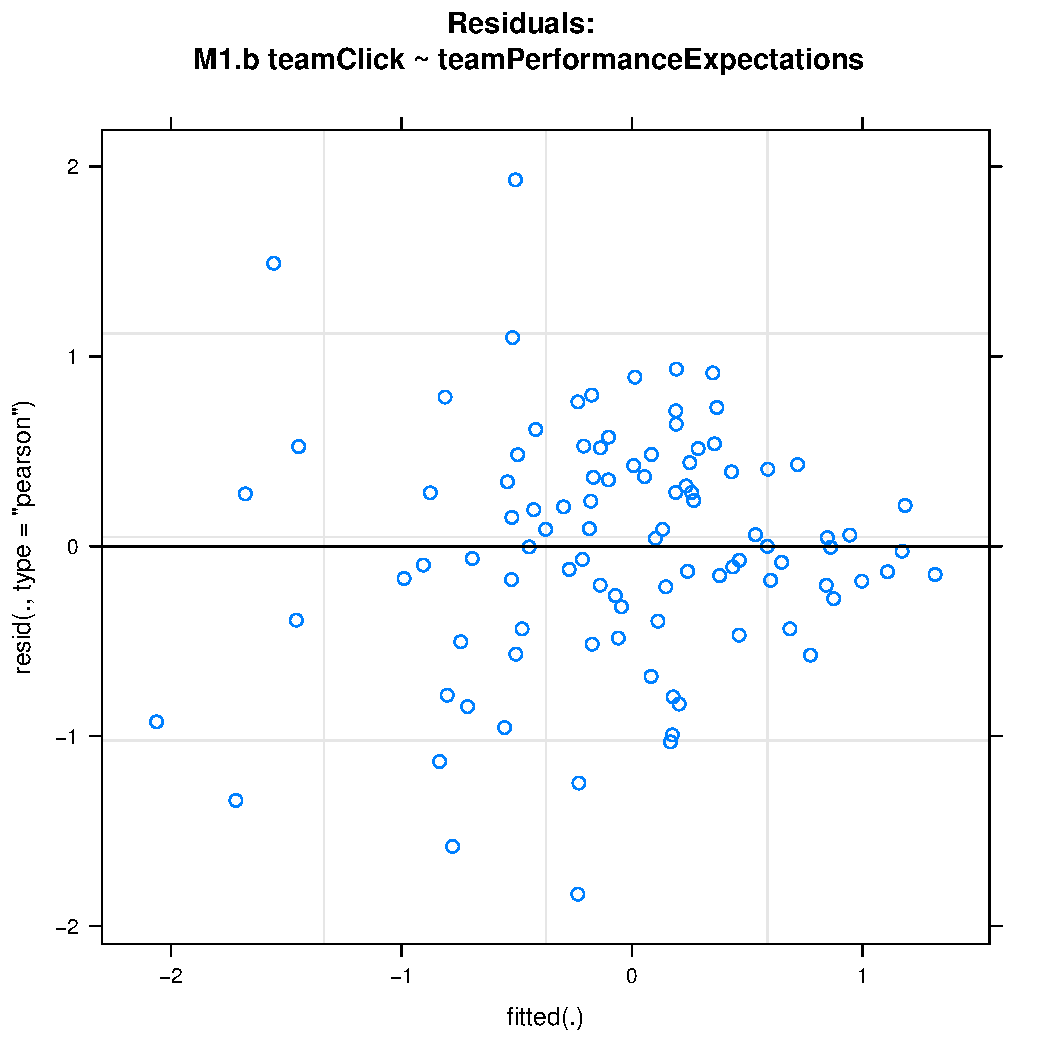
\includegraphics[scale =.4]{images/MLM1bScatter.pdf}
  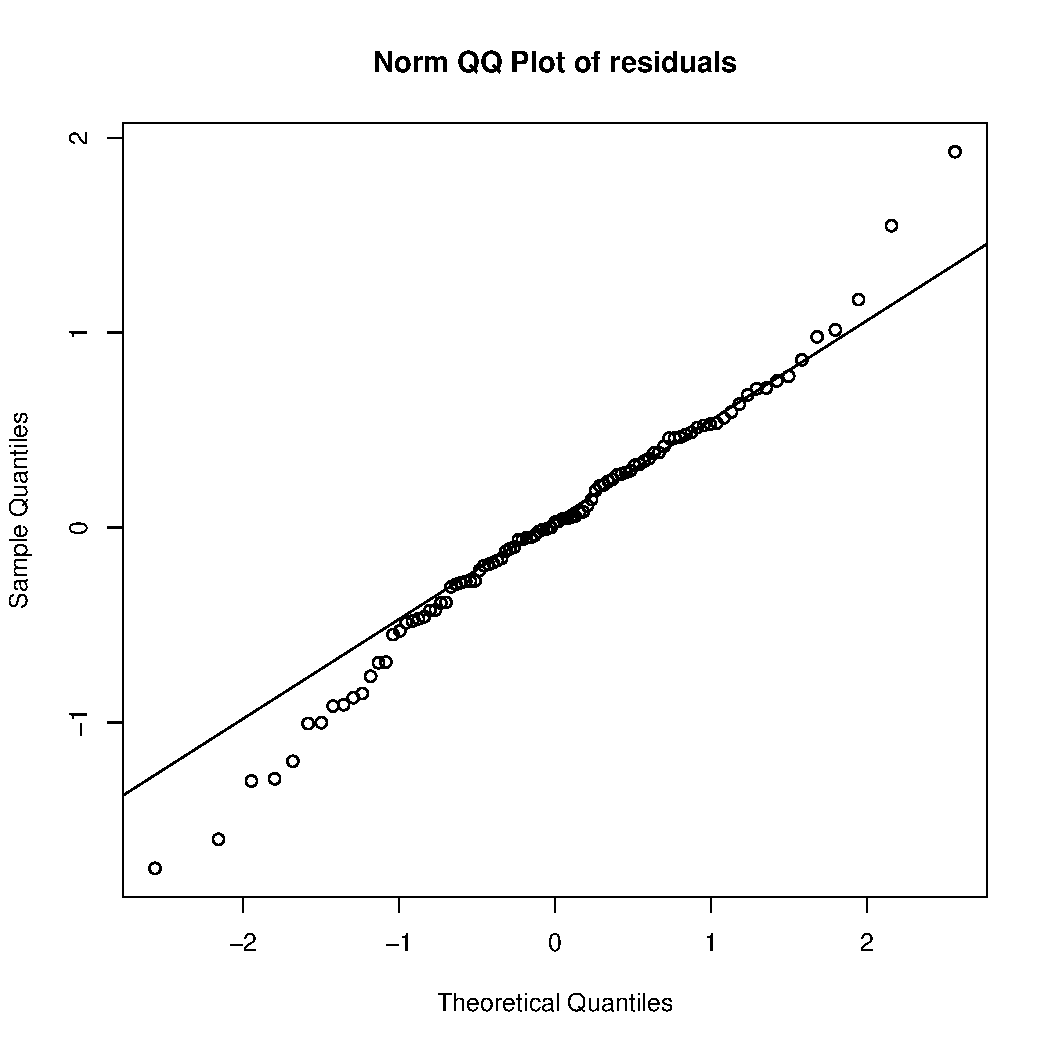
\includegraphics[scale =.4]{images/MLM1bQQNorm.pdf}
  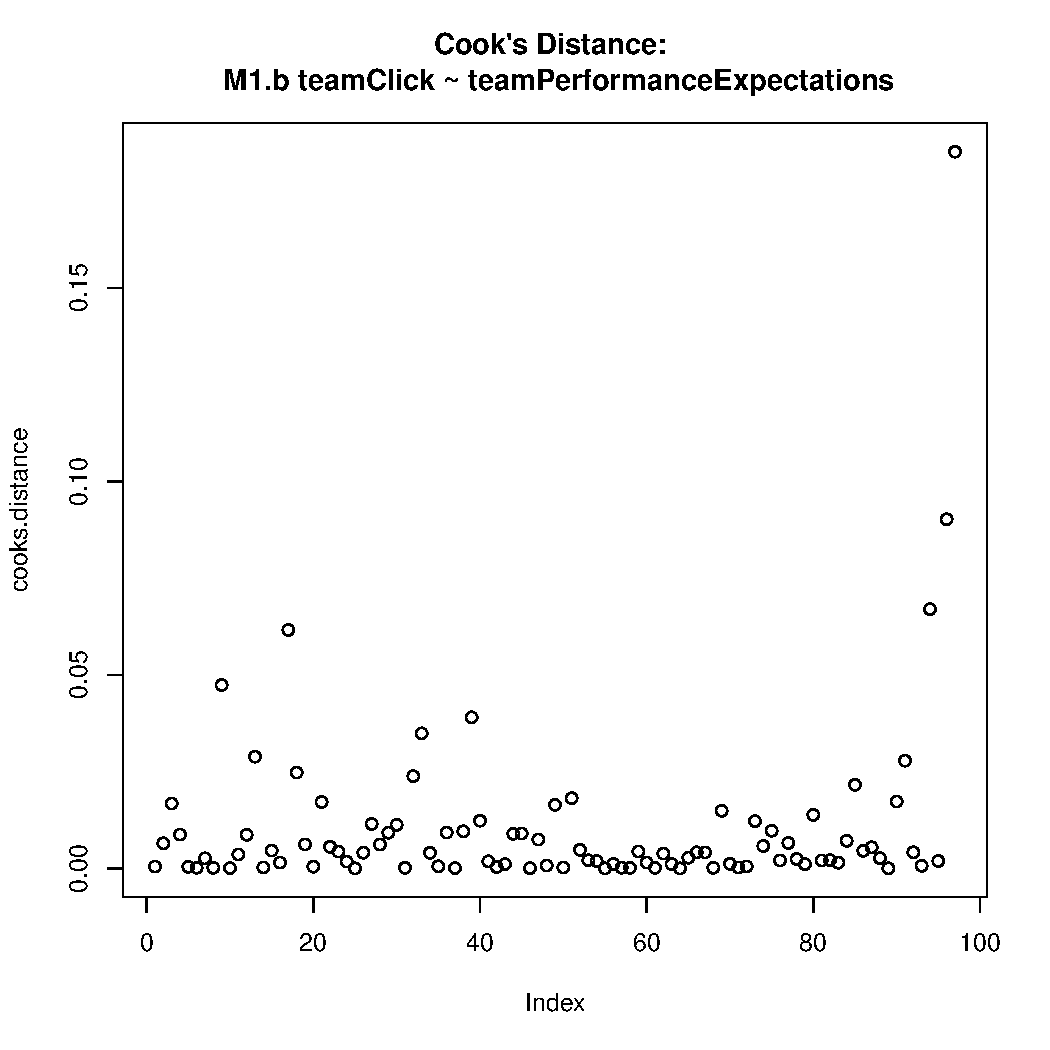
\includegraphics[scale =.4]{images/MLM1bCooksD.pdf}
  \caption{Model Assumptions: Model 1b Team Performance Expectations predict Team Click}
  \label{fig:MLM1bAssumptions}
\end{figure}





% Table created by stargazer v.5.2 by Marek Hlavac, Harvard University. E-mail: hlavac at fas.harvard.edu
% Date and time: Mon, Jun 26, 2017 - 20:35:23
\begin{table}[!htbp] \centering 
  \caption{teamClick = jointActionSuccess X teamPerformanceExpectations} 
  \label{tab:MLM1cPerformanceClickInteraction} 
\footnotesize 
\begin{tabular}{@{\extracolsep{5pt}}lc} 
\\[-1.8ex]\hline 
\hline \\[-1.8ex] 
 & \multicolumn{1}{c}{\textit{Dependent variable:}} \\ 
\cline{2-2} 
\\[-1.8ex] & teamClick \\ 
\hline \\[-1.8ex] 
 (constant) & $-$0.83$^{*}$ \\ 
  & (0.41) \\ 
  & \\ 
 jointActionSuccess & 0.57$^{*}$ \\ 
  & (0.25) \\ 
  & \\ 
 teamPerformanceExpectations & 0.01 \\ 
  & (0.005) \\ 
  & \\ 
 indPerformanceSuccess & 0.01 \\ 
  & (0.10) \\ 
  & \\ 
 indPerformanceExpectations & $-$0.001 \\ 
  & (0.003) \\ 
  & \\ 
 objectiveCompetence & 0.06 \\ 
  & (0.08) \\ 
  & \\ 
 subjectiveCompetence & 0.10 \\ 
  & (0.07) \\ 
  & \\ 
 finalRank & 0.03 \\ 
  & (0.04) \\ 
  & \\ 
 minutesTotal & 0.01 \\ 
  & (0.003) \\ 
  & \\ 
 pointsTotal & 0.004 \\ 
  & (0.01) \\ 
  & \\ 
 teamPerformanceComponentsFactorPost:teamPerformance7 & 0.0001 \\ 
  & (0.003) \\ 
  & \\ 
\hline \\[-1.8ex] 
Marginal R-squared & .56 \\ 
Conditional R-squared & .65 \\ 
Observations & 97 \\ 
Log Likelihood & $-$90.96 \\ 
Akaike Inf. Crit. & 217.91 \\ 
Bayesian Inf. Crit. & 264.26 \\ 
\hline 
\hline \\[-1.8ex] 
\textit{Note:}  & \multicolumn{1}{r}{$^{*}$p$<$0.05; $^{**}$p$<$0.01; $^{***}$p$<$0.001} \\ 
\end{tabular} 
\end{table} 






\begin{figure}[htbp]
  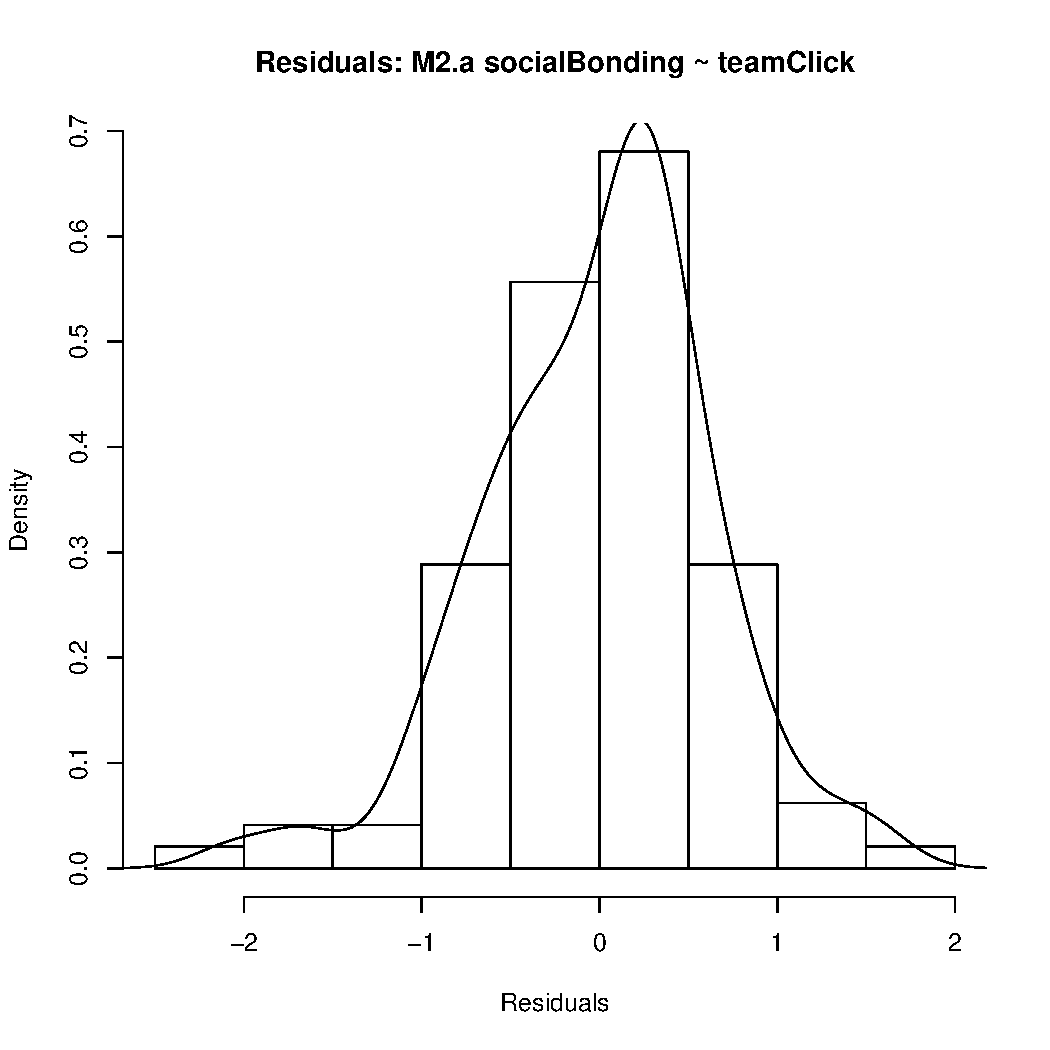
\includegraphics[scale =.4]{images/MLM2aHist.pdf}
  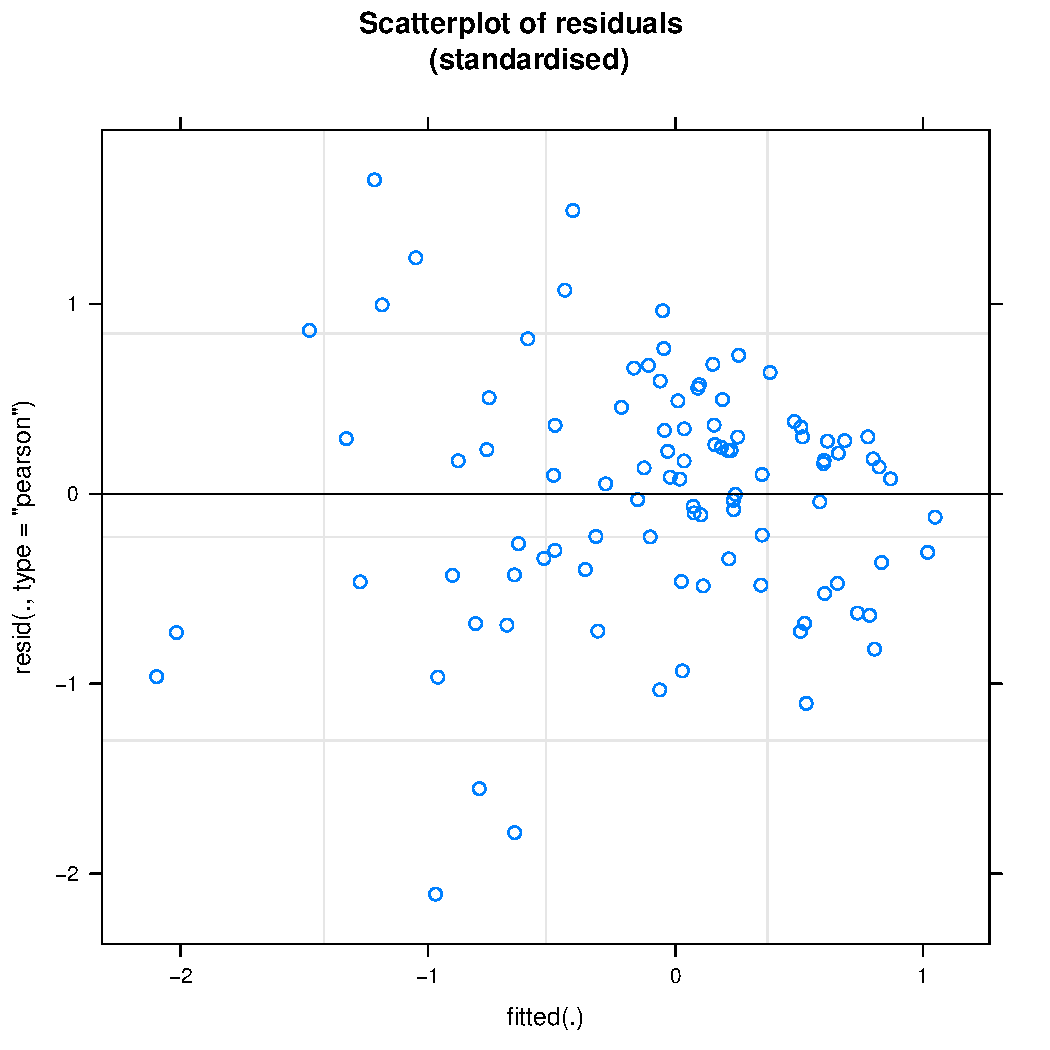
\includegraphics[scale =.4]{images/MLM2aScatter.pdf}
  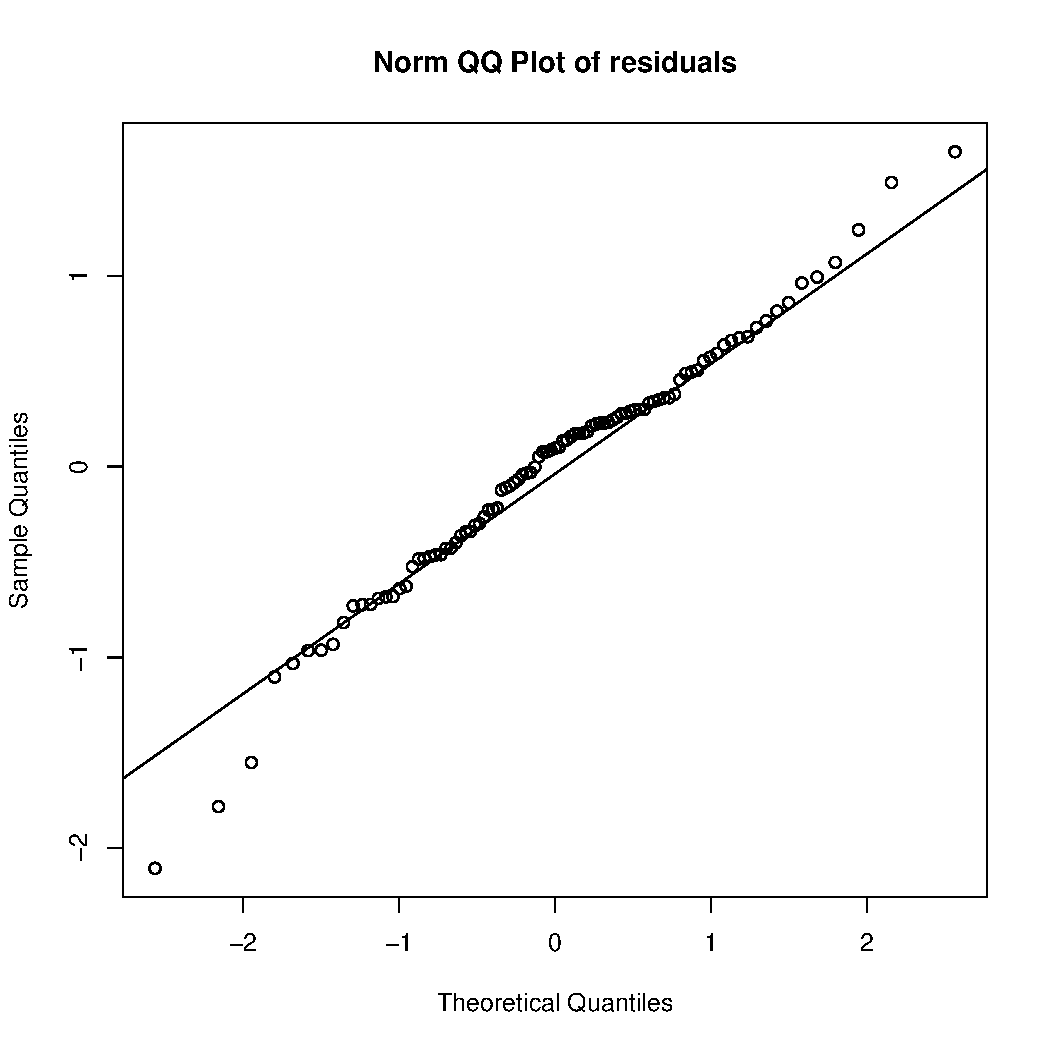
\includegraphics[scale =.4]{images/MLM2aQQNorm.pdf}
  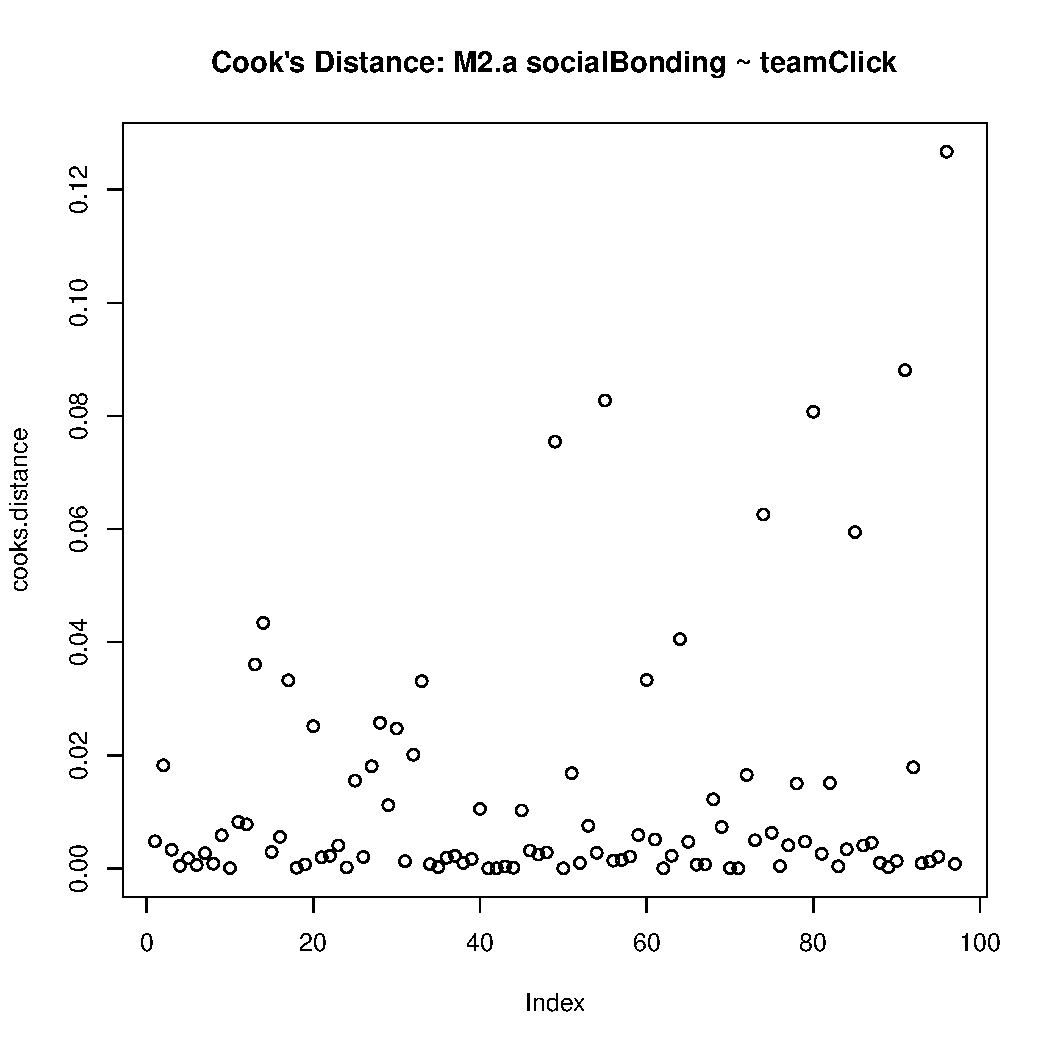
\includegraphics[scale =.4]{images/MLM2aCooksD.pdf}
  \caption{Model Assumptions: M2a Team Click predicts Social Bonding}
  \label{fig:MKM2aAssumptions}
\end{figure}





\begin{figure}[htbp]
  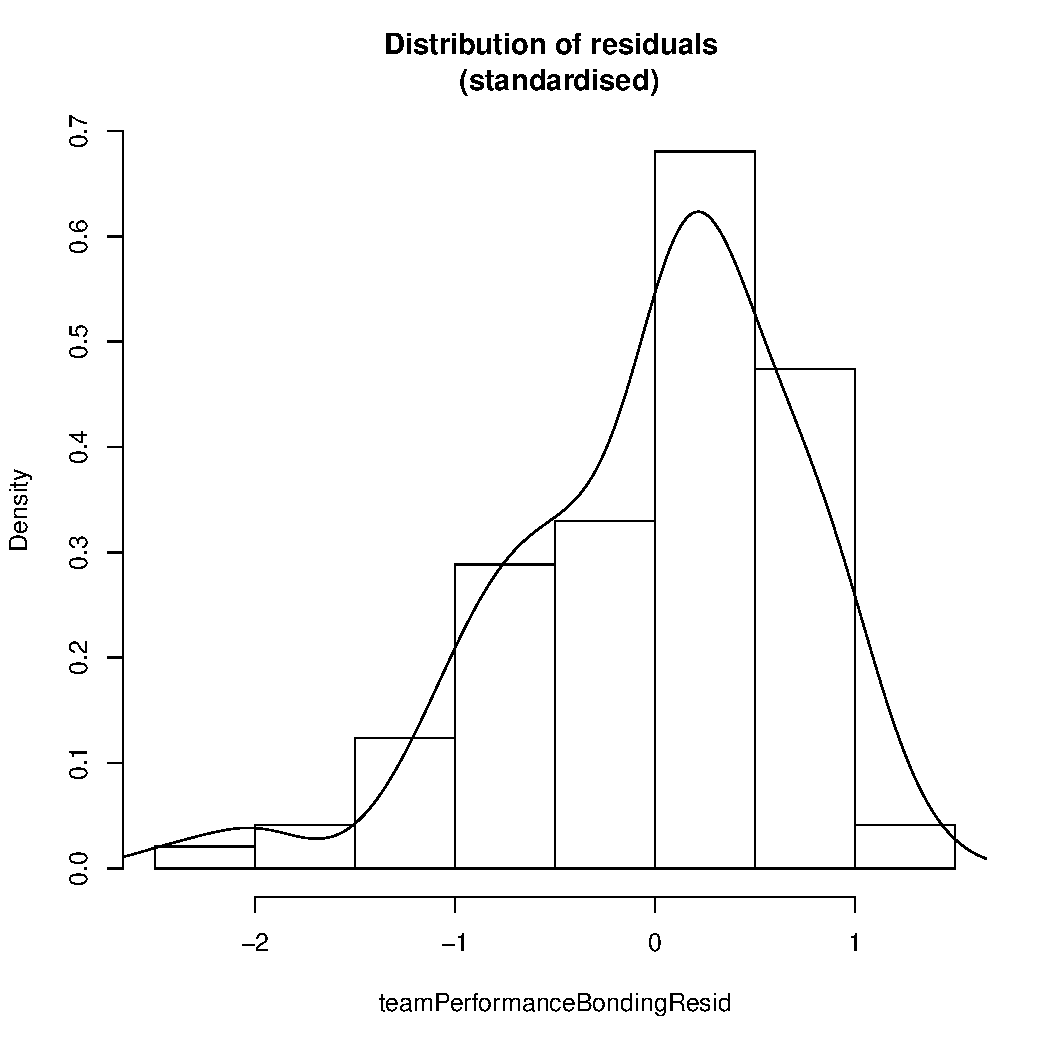
\includegraphics[scale =.4]{images/MLM3aHist.pdf}
  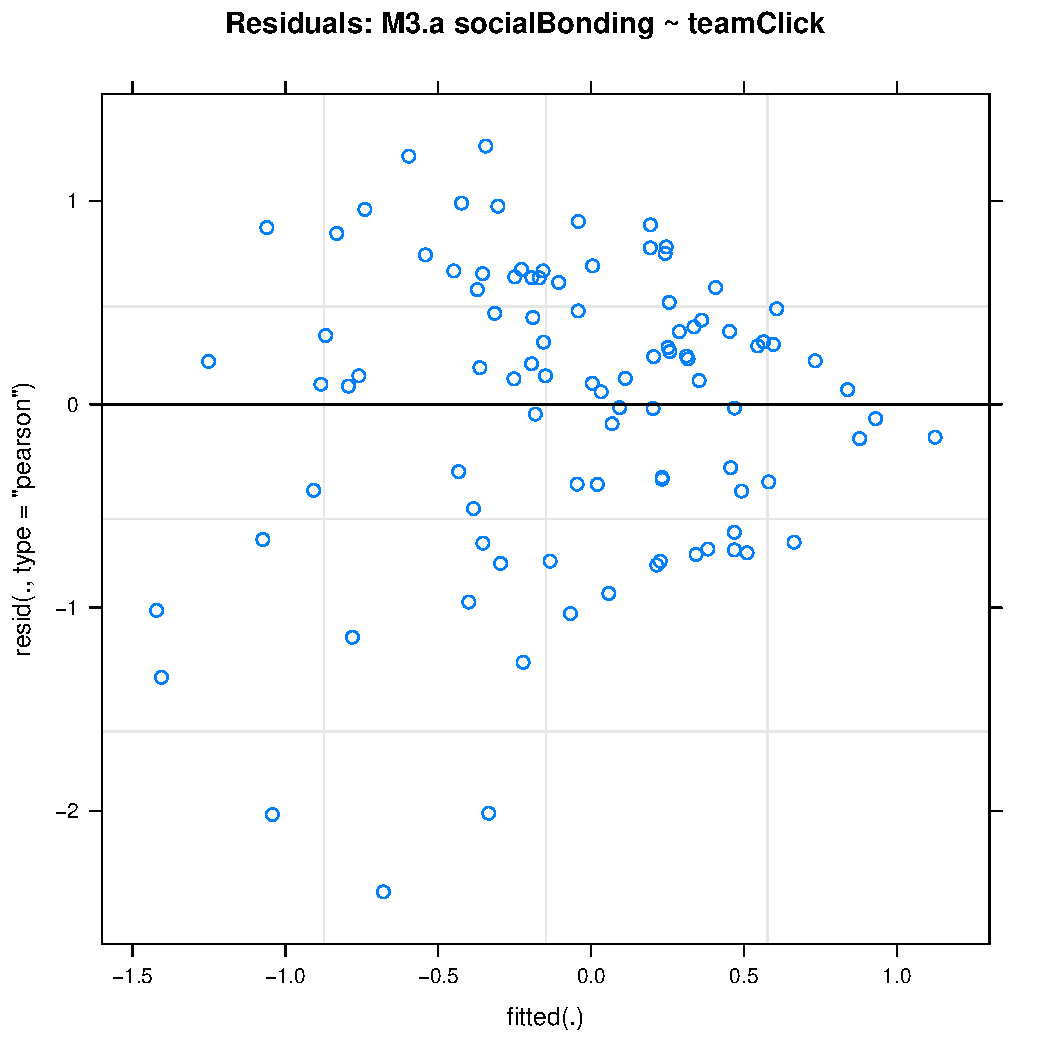
\includegraphics[scale =.4]{images/MLM3aScatter.pdf}
  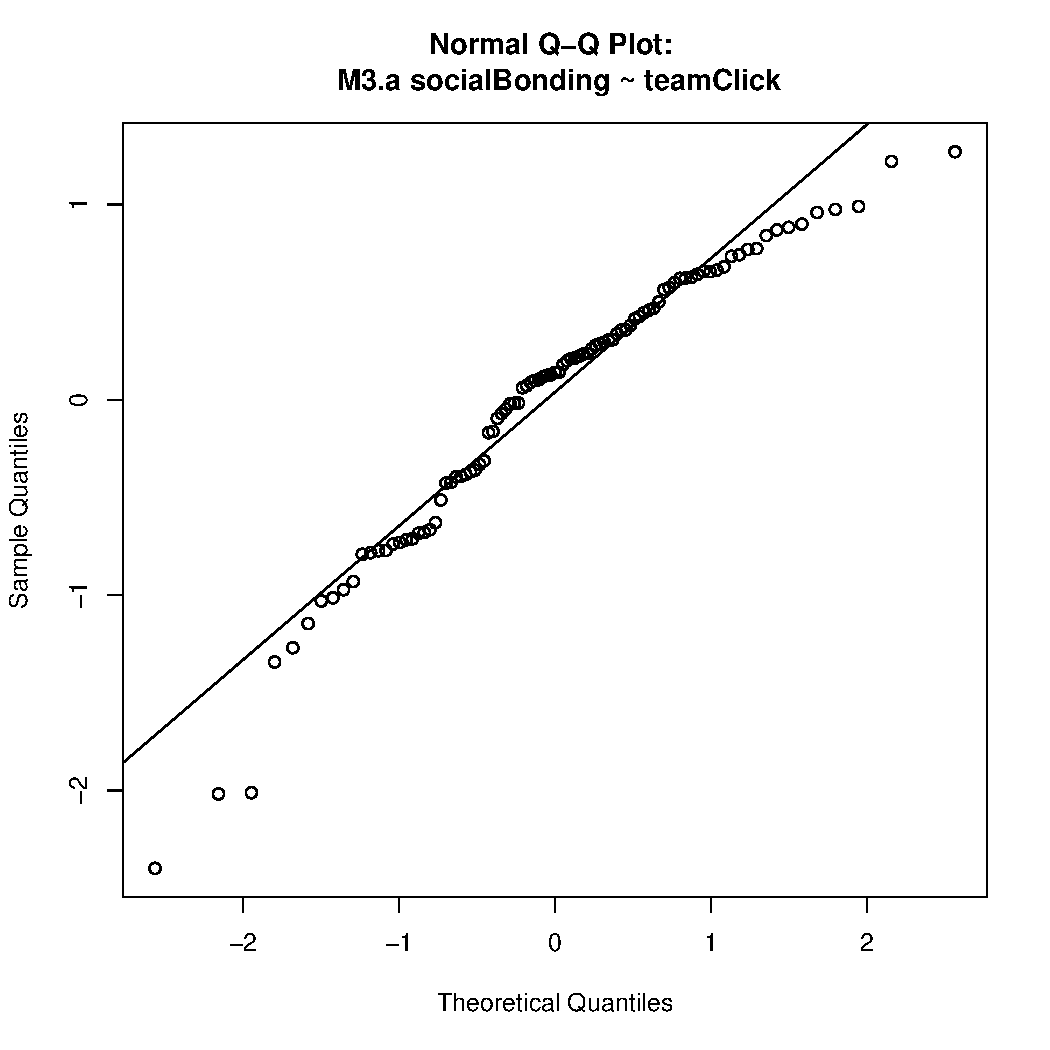
\includegraphics[scale =.4]{images/MLM3aQQNorm.pdf}
  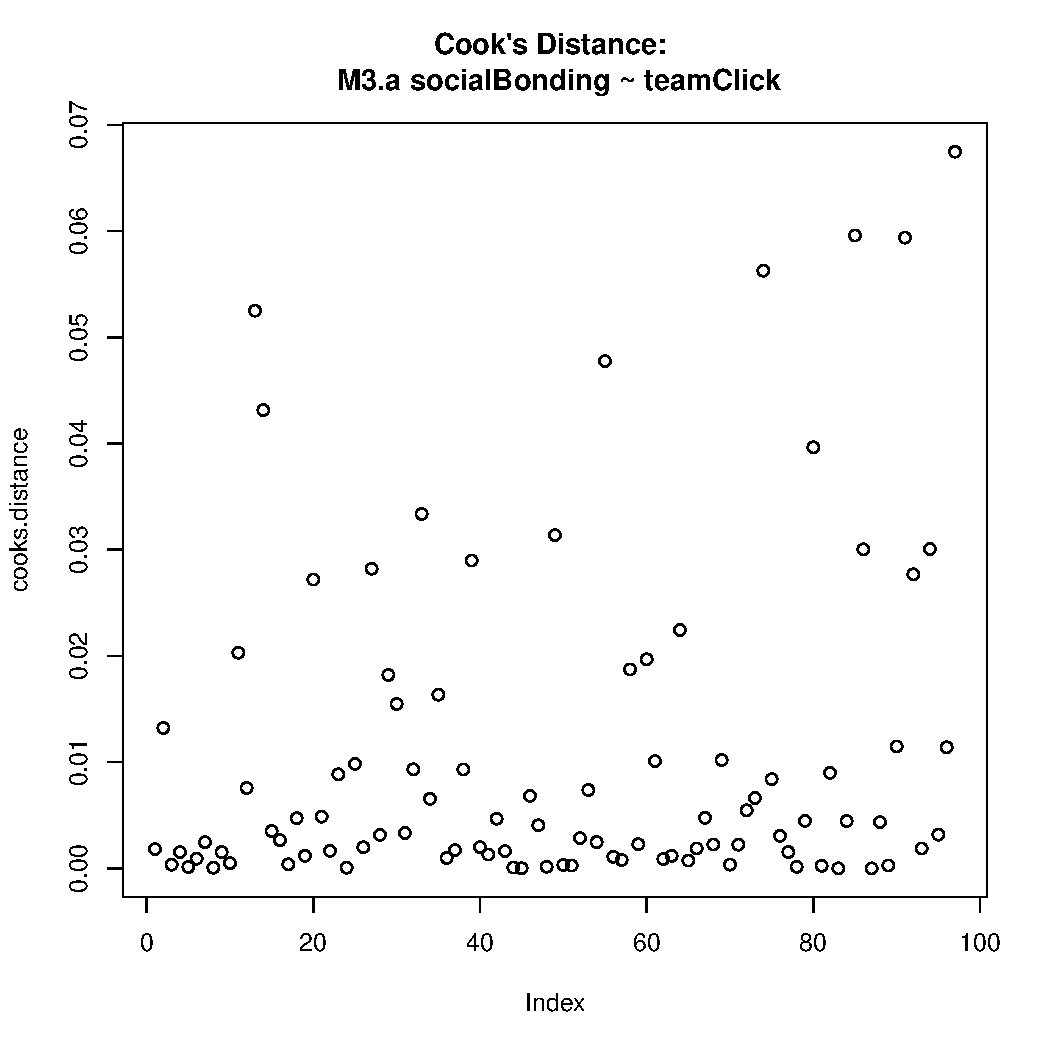
\includegraphics[scale =.4]{images/MLM3aCooksD.pdf}
  \caption{Model Assumptions: M3a Joint Action Success predicts Social Bonding}
  \label{fig:MLM3aAssumptions}
\end{figure}

\begin{figure}[htbp]
  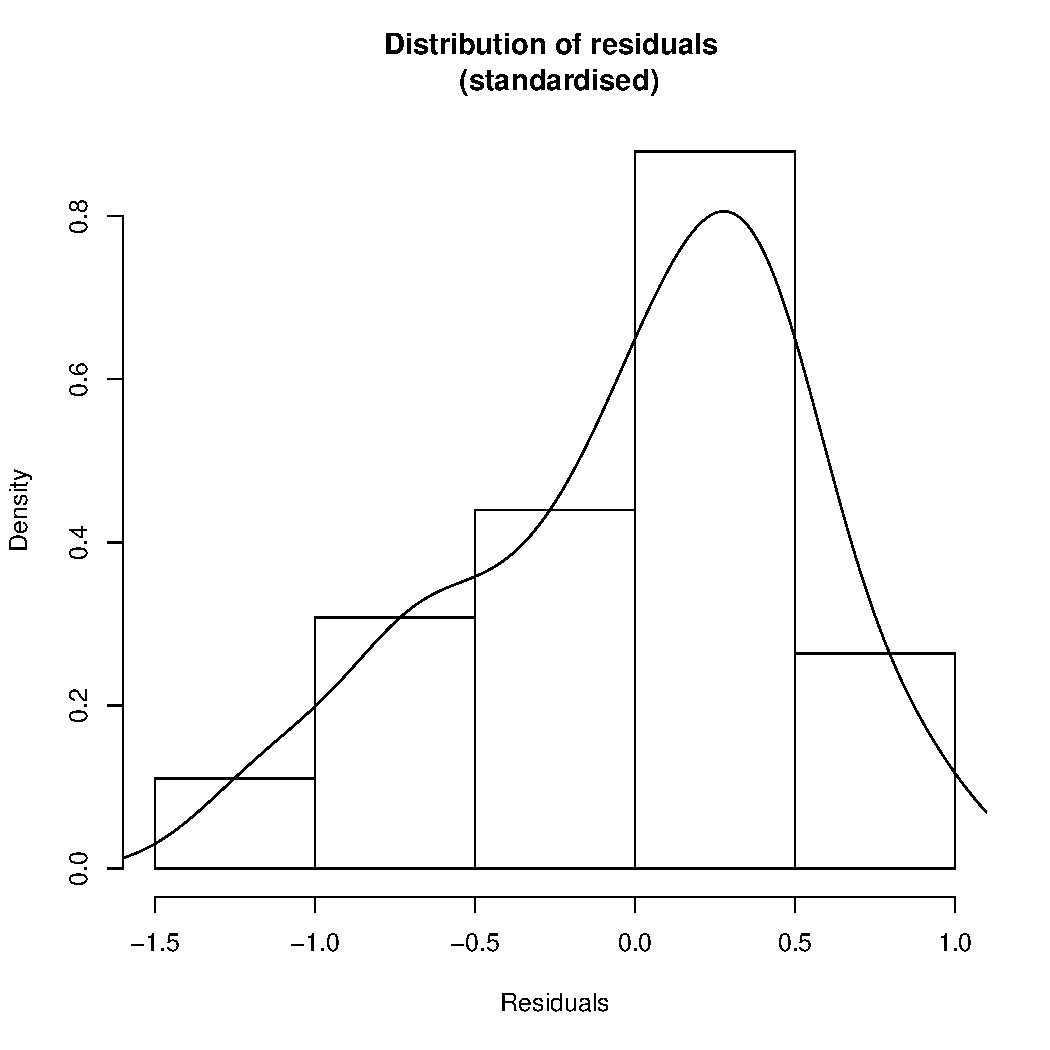
\includegraphics[scale =.4]{images/MLM3aOutHist.pdf}
  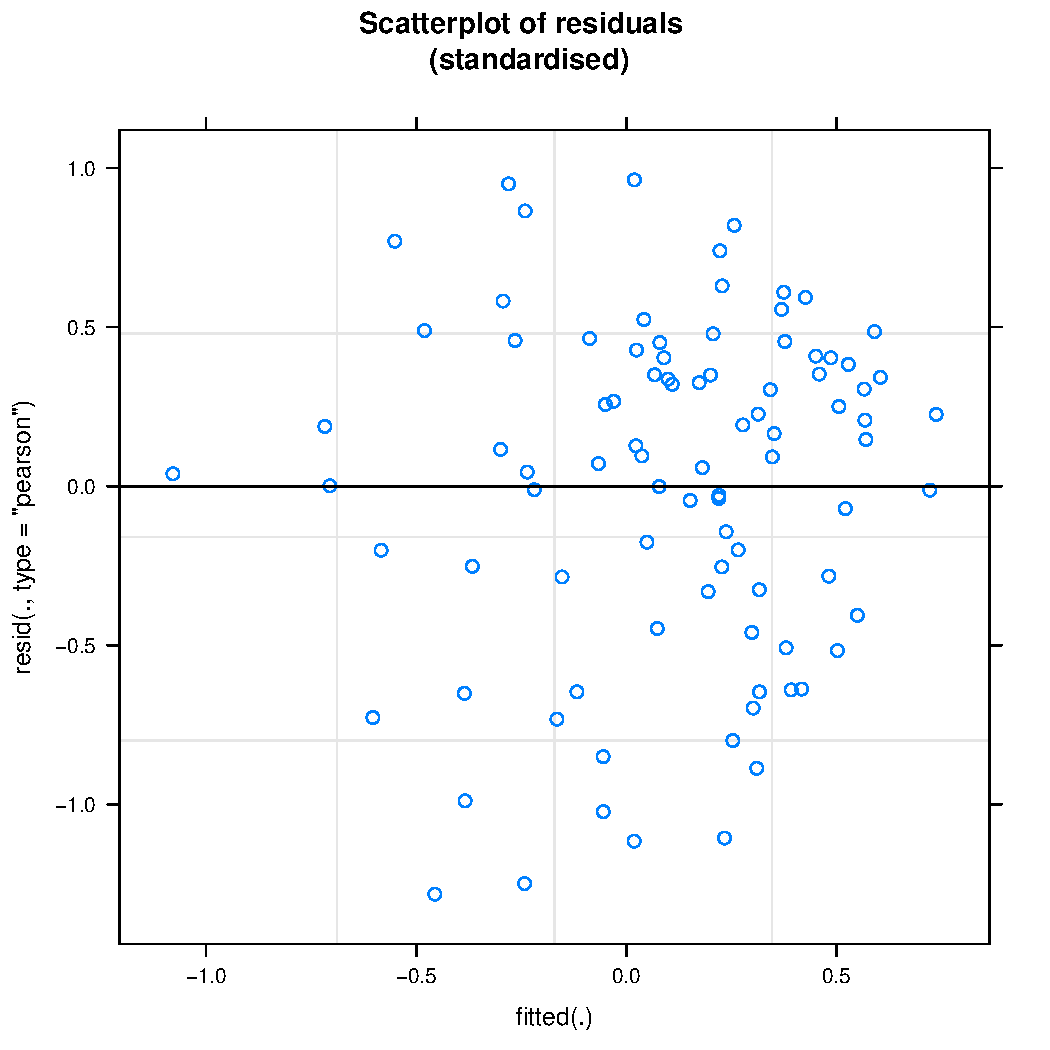
\includegraphics[scale =.4]{images/MLM3aOutScatter.pdf}
  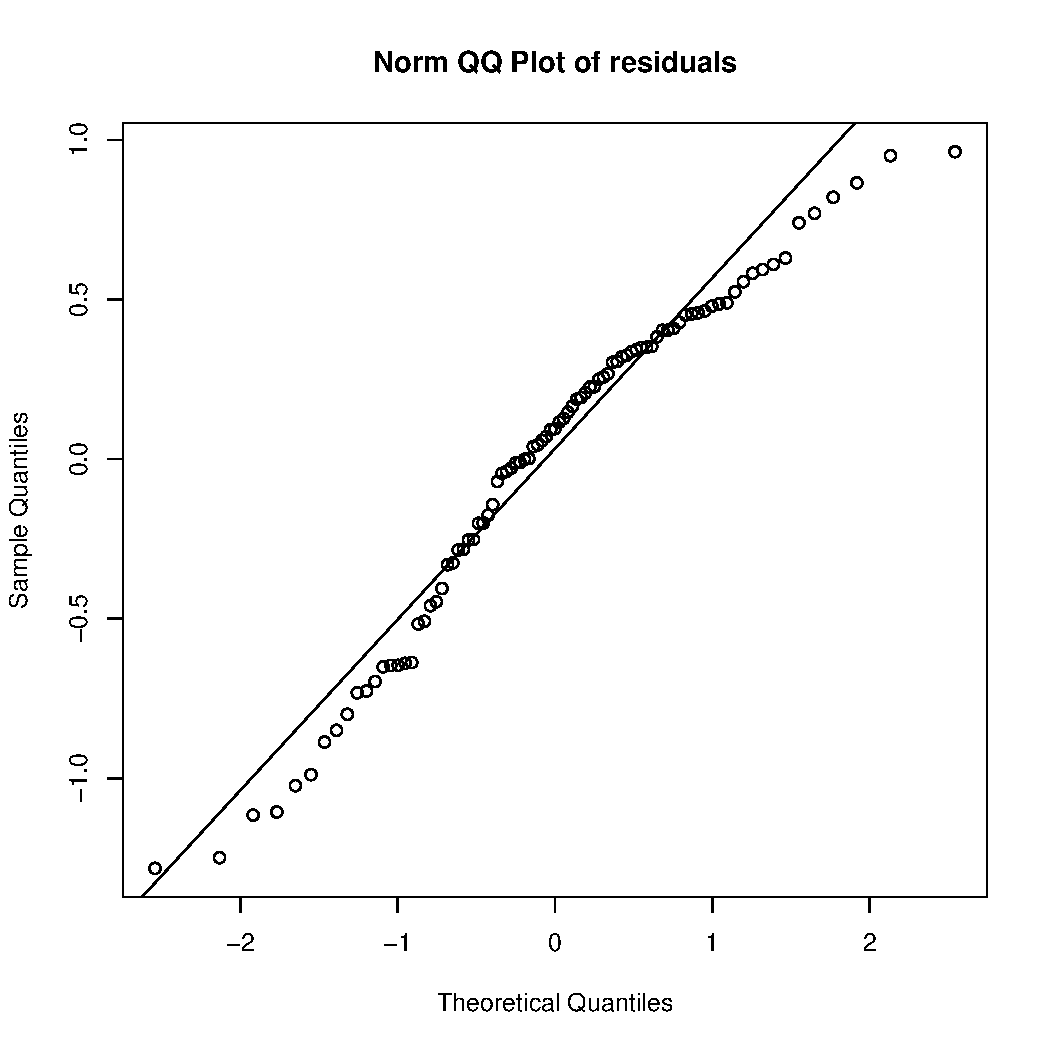
\includegraphics[scale =.4]{images/MLM3aOutQQNorm.pdf}
  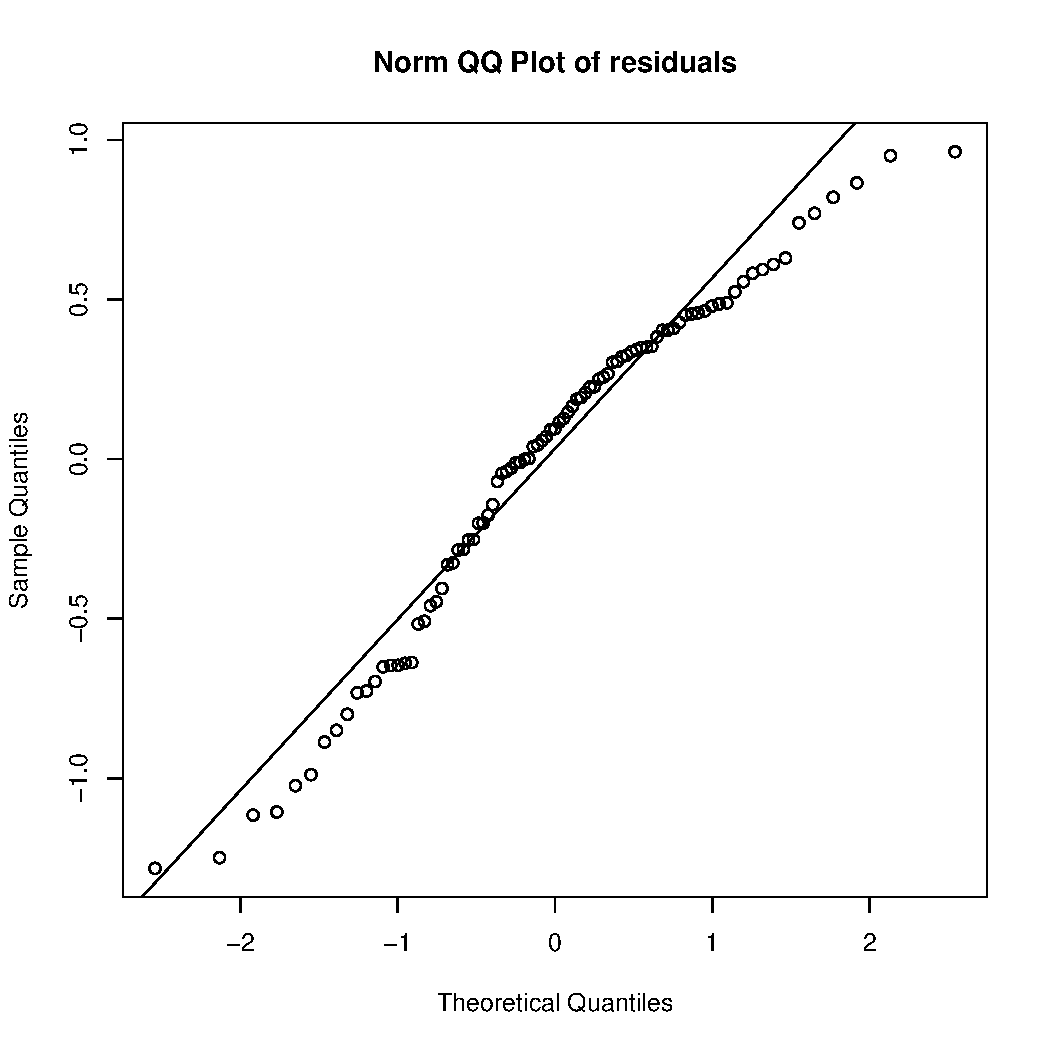
\includegraphics[scale =.4]{images/MLM3aOutCooksD.pdf}
  \caption{Model Assumptions: M3a Joint Action Success predicts Social Bonding (outliers removed)}
  \label{fig:MLM3aOutAssumptions}
\end{figure}

\begin{figure}[htbp]
  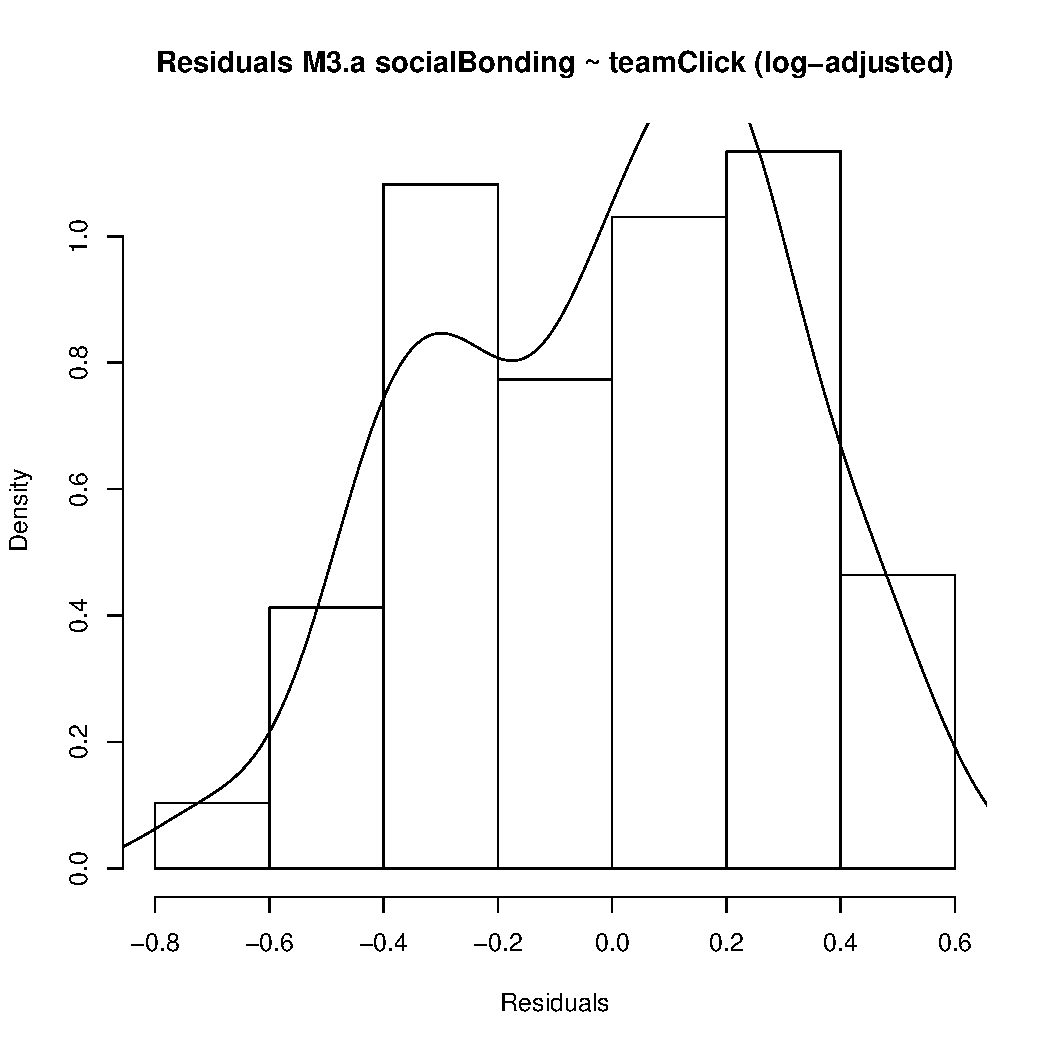
\includegraphics[scale =.4]{images/MLM3aLogHist.pdf}
  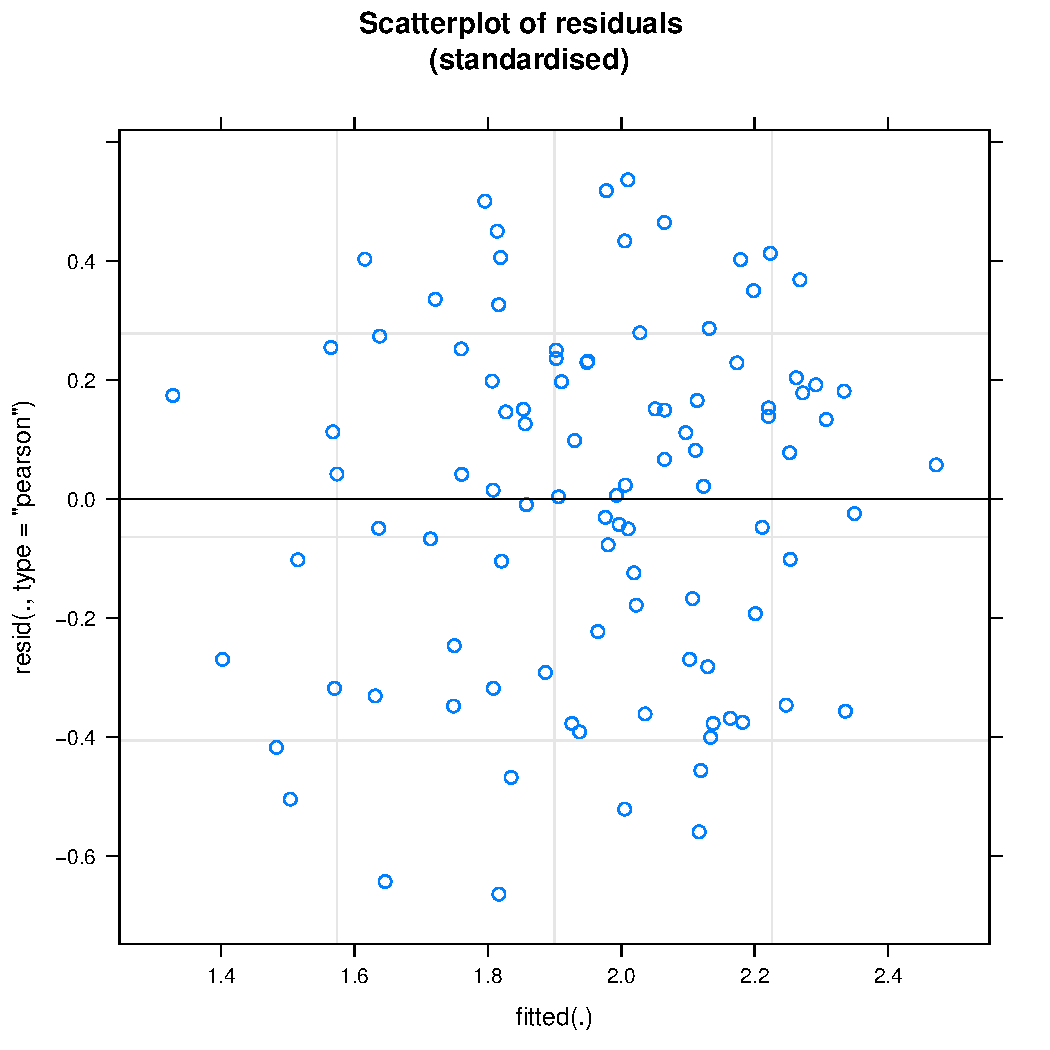
\includegraphics[scale =.4]{images/MLM3aLogScatter.pdf}
  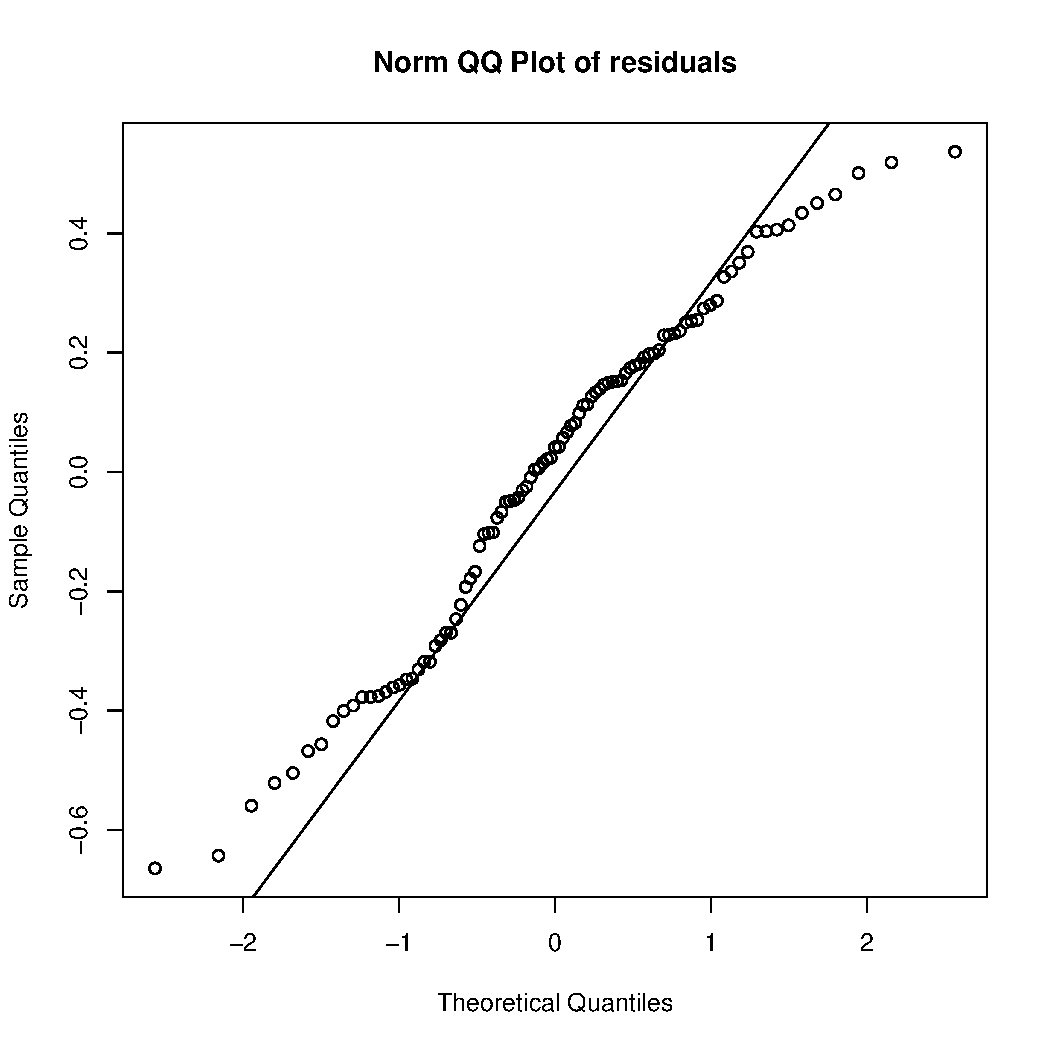
\includegraphics[scale =.4]{images/MLM3aLogQQNorm.pdf}
  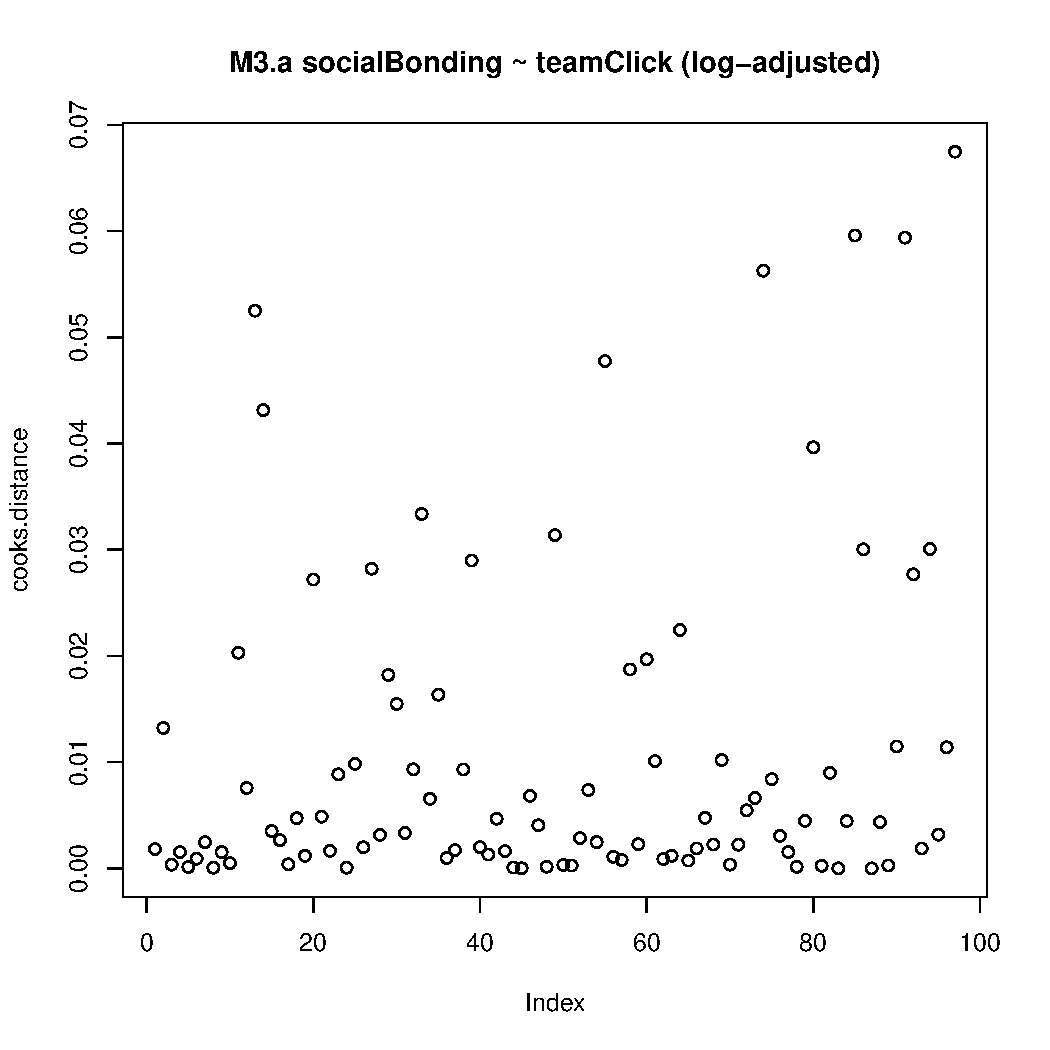
\includegraphics[scale =.4]{images/MLM3aLogCooksD.pdf}
  \caption{Model Assumptions: M3a Joint Action Success predicts Social Bonding (log-transformed)}
  \label{fig:MLM3aLogAssumptions}
\end{figure}








\begin{figure}[htbp]
  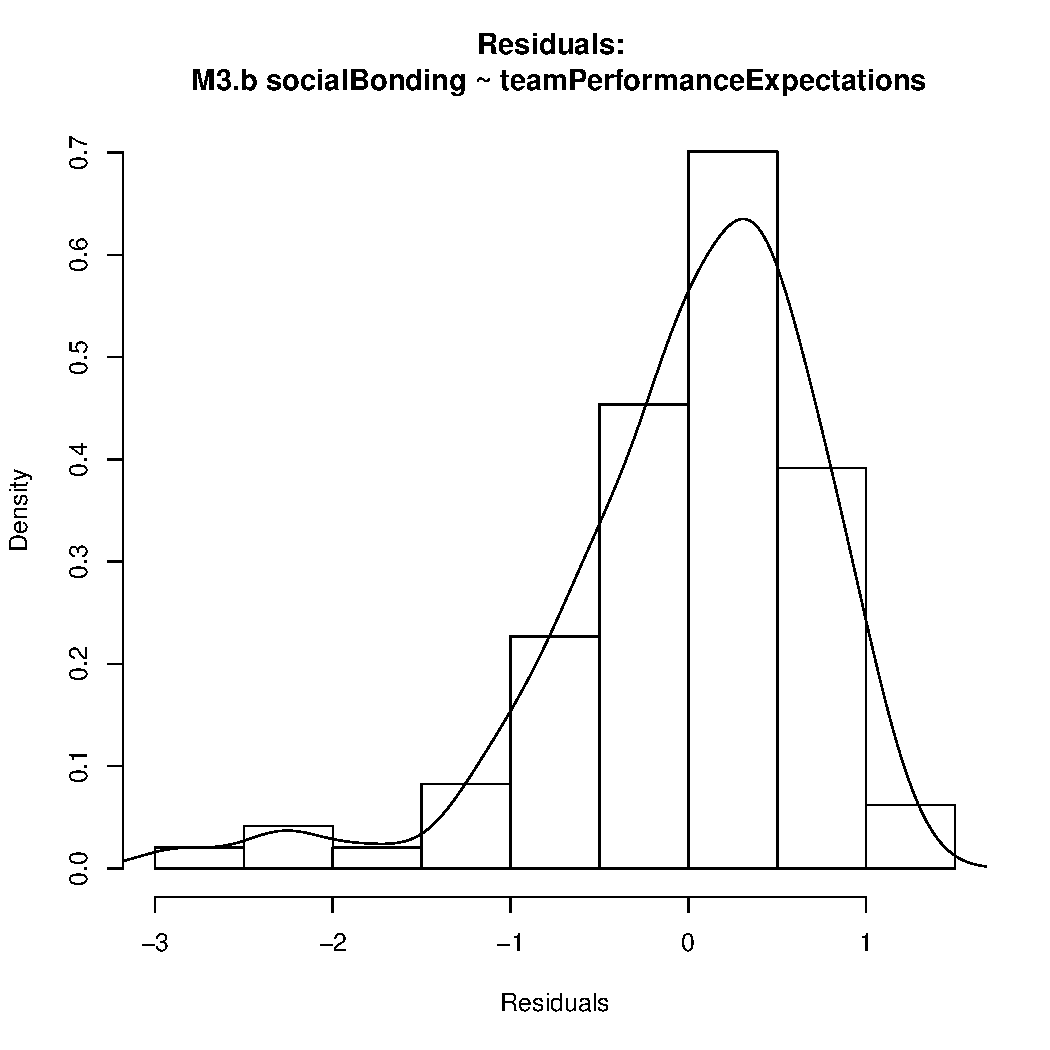
\includegraphics[scale =.4]{images/MLM3bHist.pdf}
  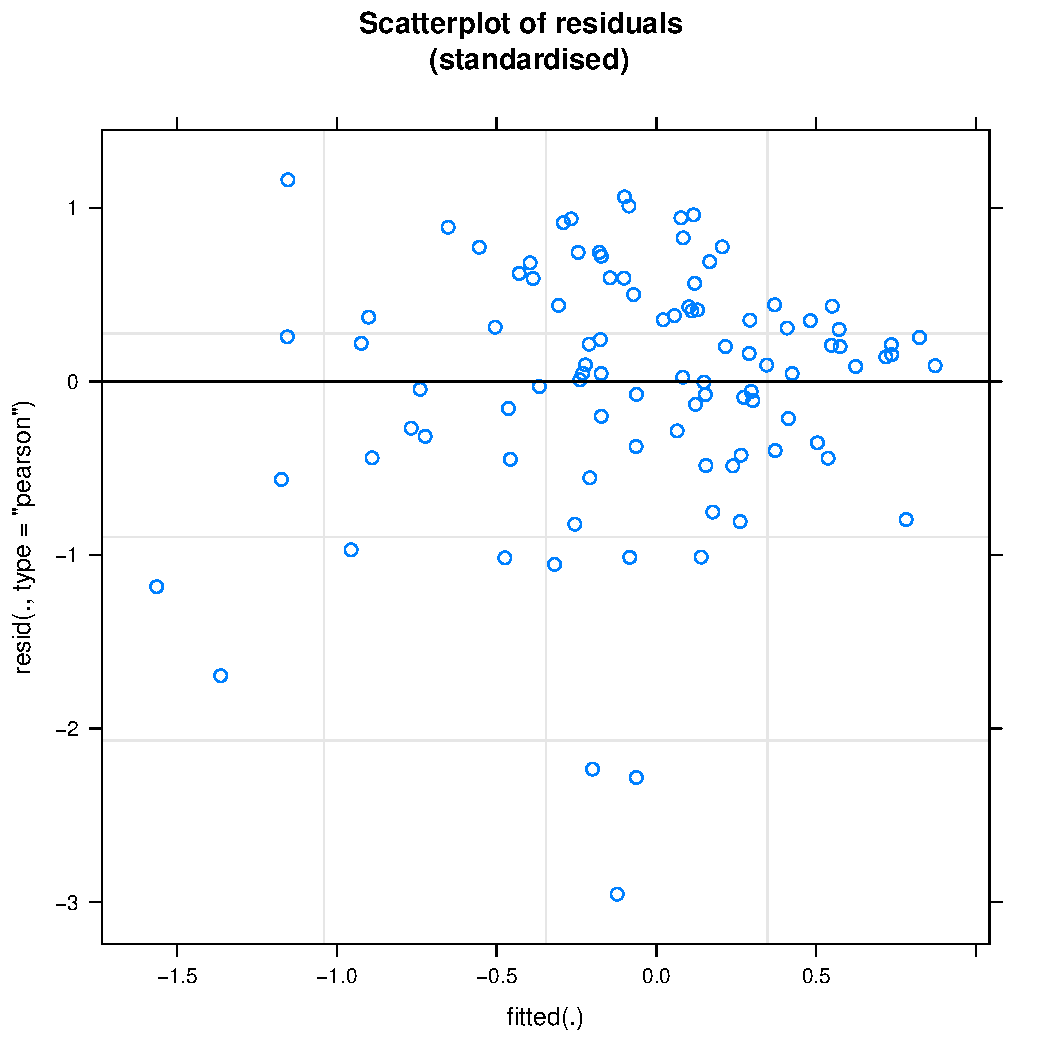
\includegraphics[scale =.4]{images/MLM3bScatter.pdf}
  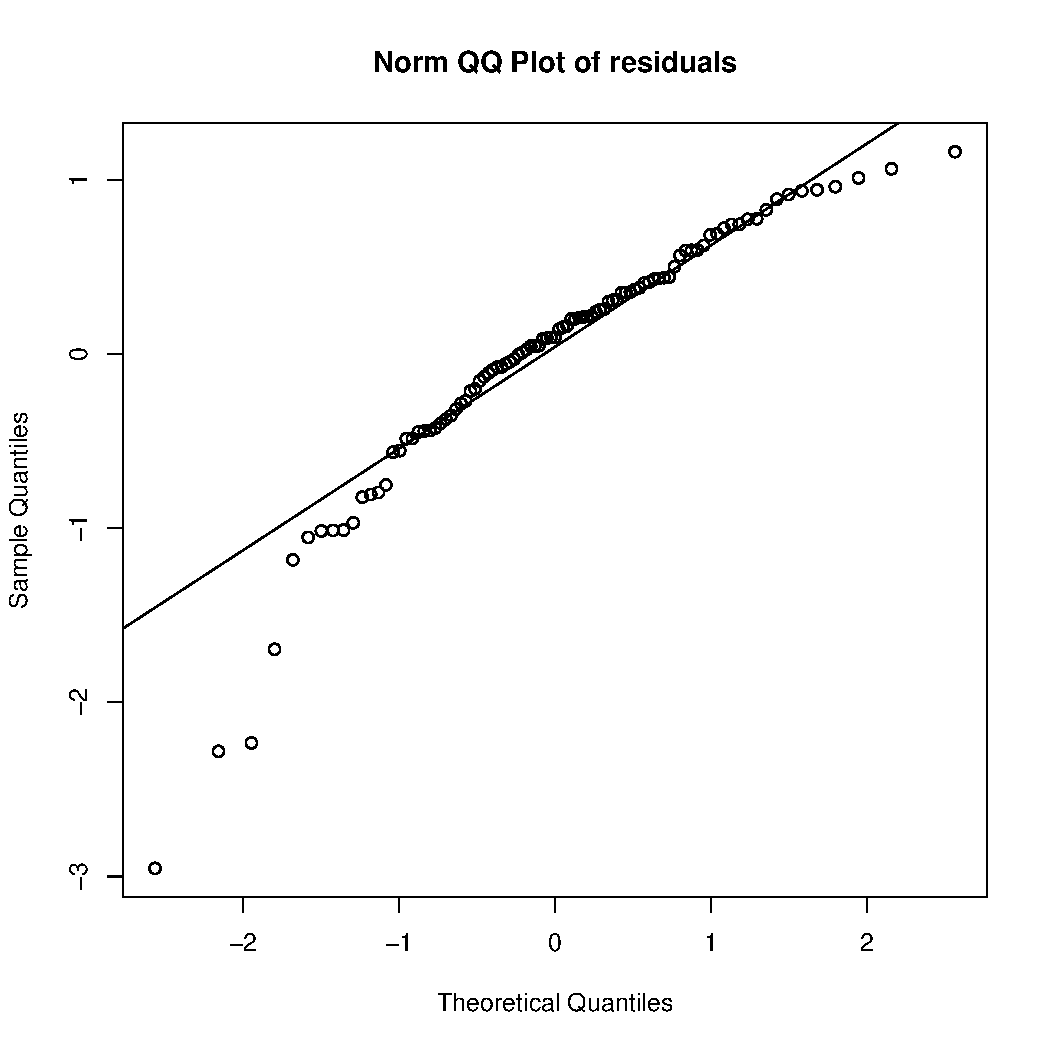
\includegraphics[scale =.4]{images/MLM3bQQNorm.pdf}
  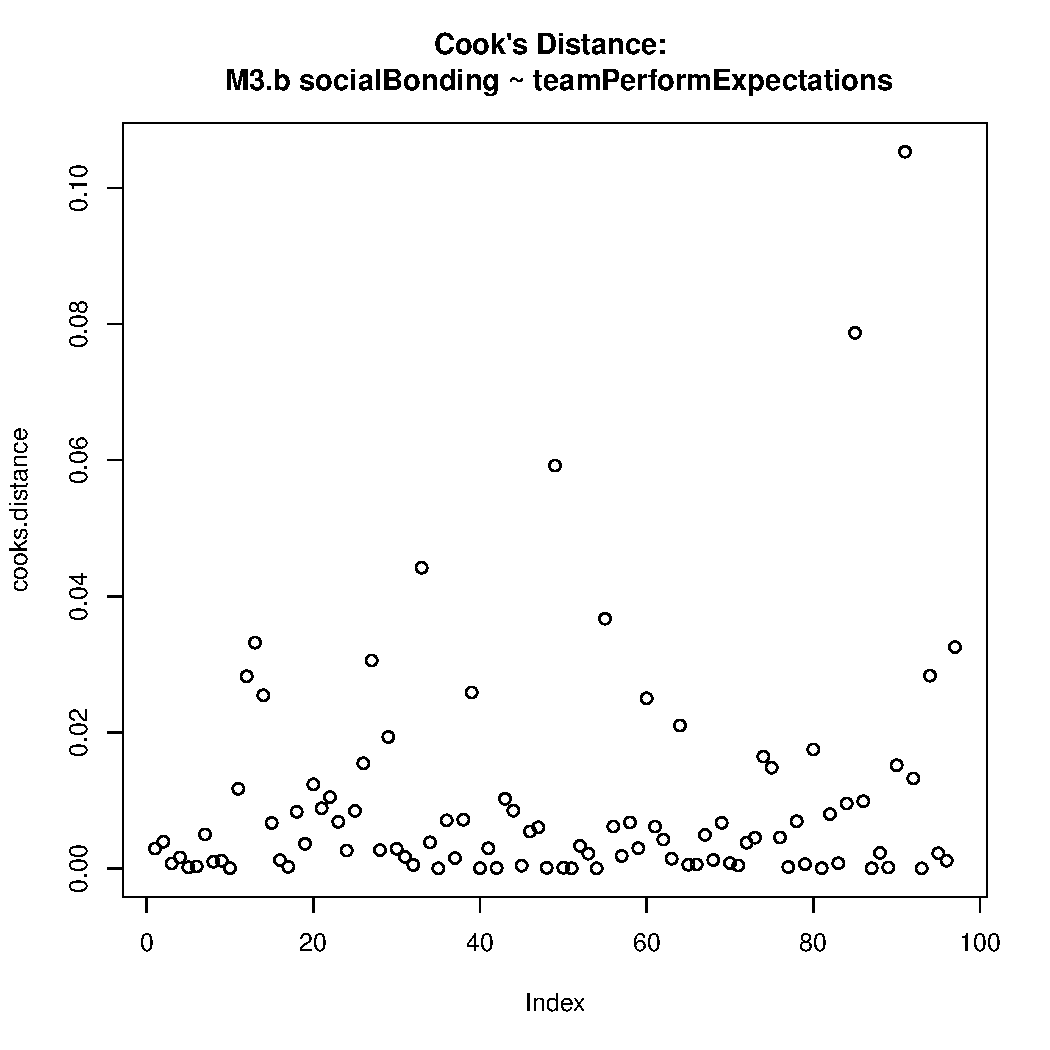
\includegraphics[scale =.4]{images/MLM3bCooksD.pdf}
  \caption{Model Assumptions: M3a Joint Action Success predicts Social Bonding (log-transformed)}
  \label{fig:MLM3bAssumptions}
\end{figure}

\begin{figure}[htbp]
  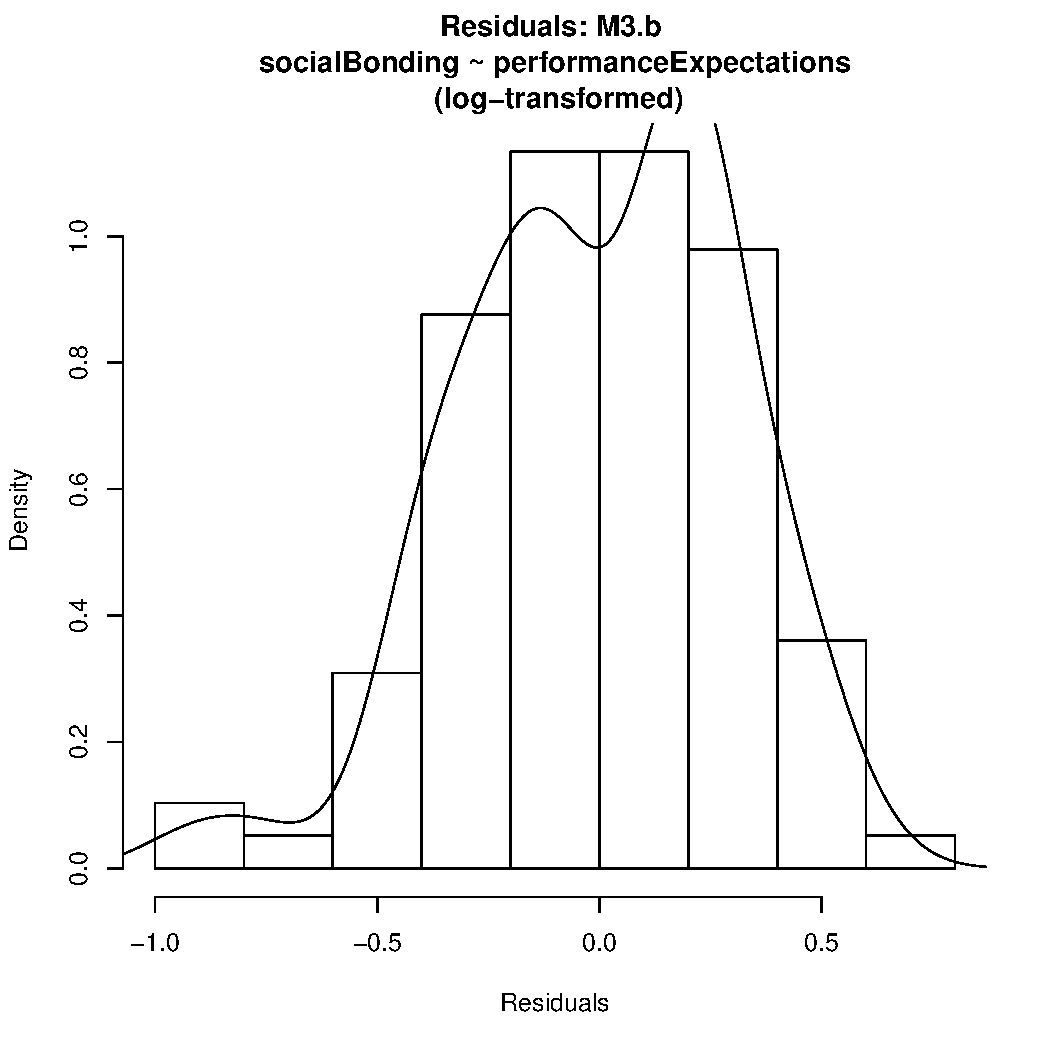
\includegraphics[scale =.4]{images/MLM3bLogHist.pdf}
  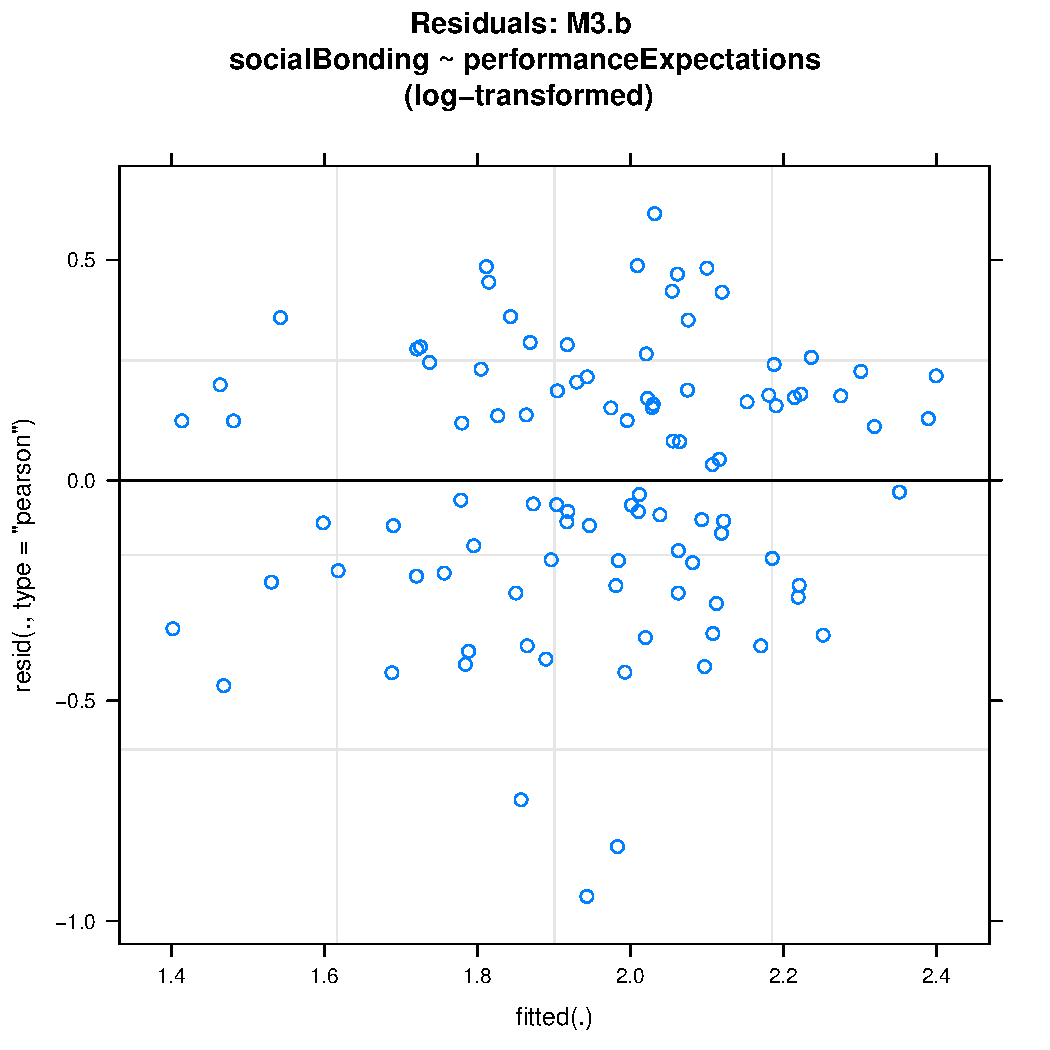
\includegraphics[scale =.4]{images/MLM3bLogScatter.pdf}
  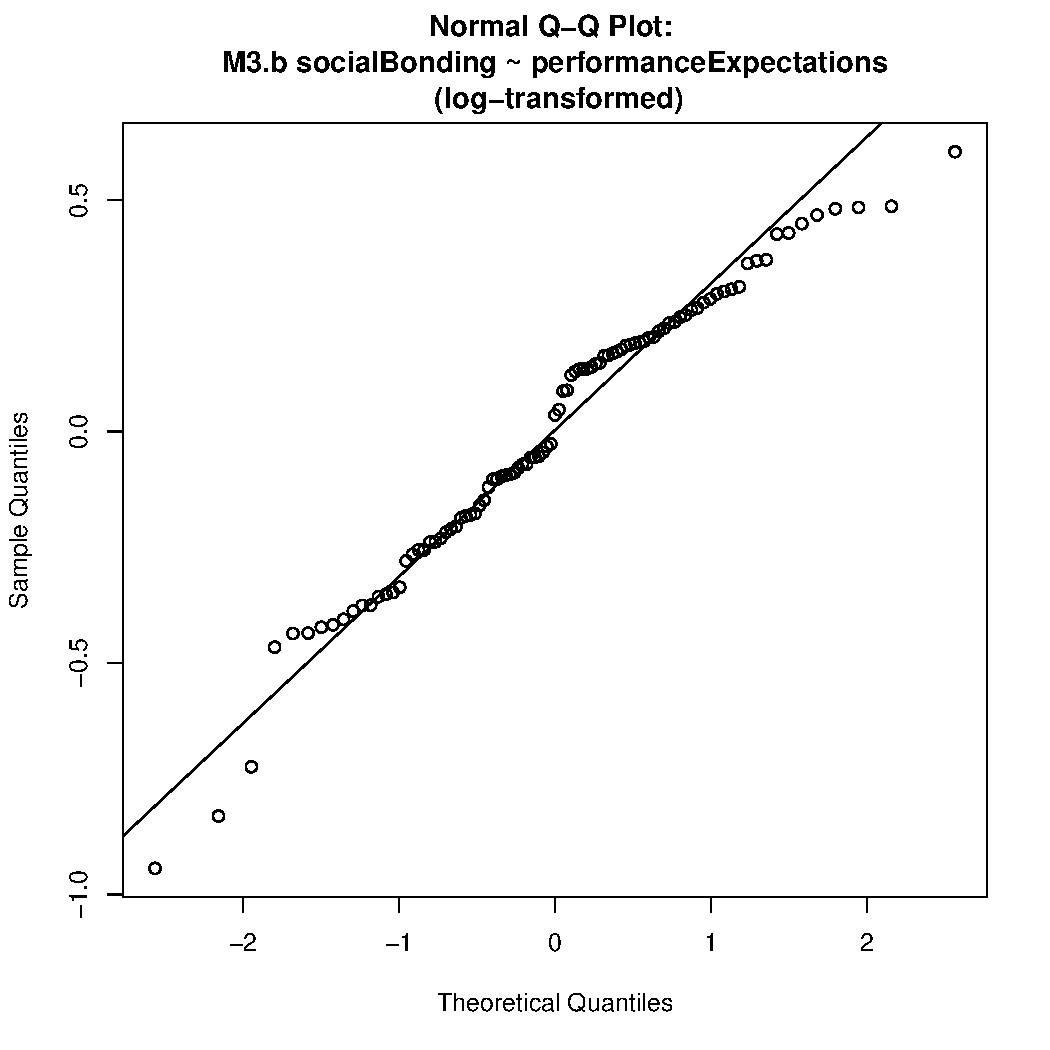
\includegraphics[scale =.4]{images/MLM3bLogQQNorm.pdf}
  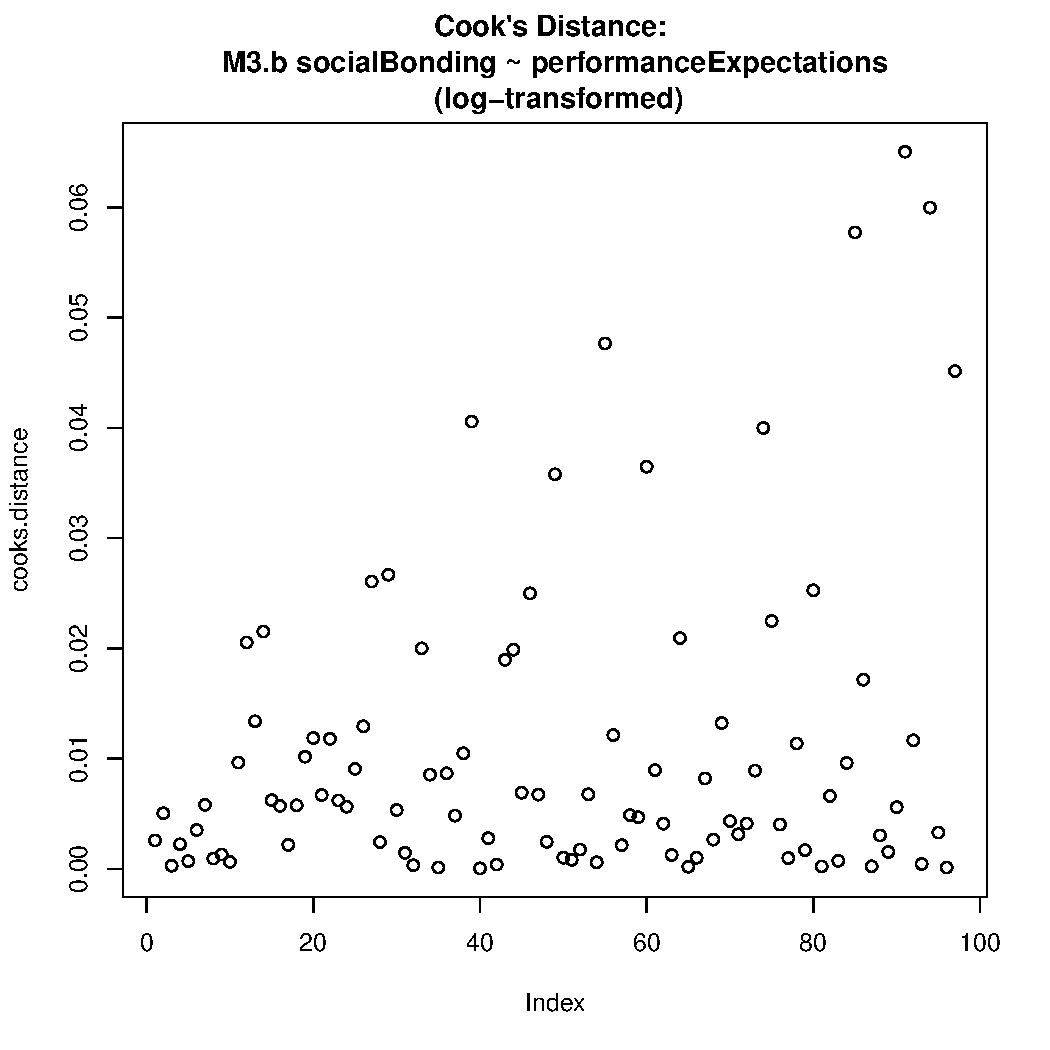
\includegraphics[scale =.4]{images/MLM3bLogCooksD.pdf}
  \caption{Model Assumptions: M3a Joint Action Success predicts Social Bonding (log-transformed)}
  \label{fig:MLM3bLogAssumptions}
\end{figure}






\begin{figure}[htbp]
  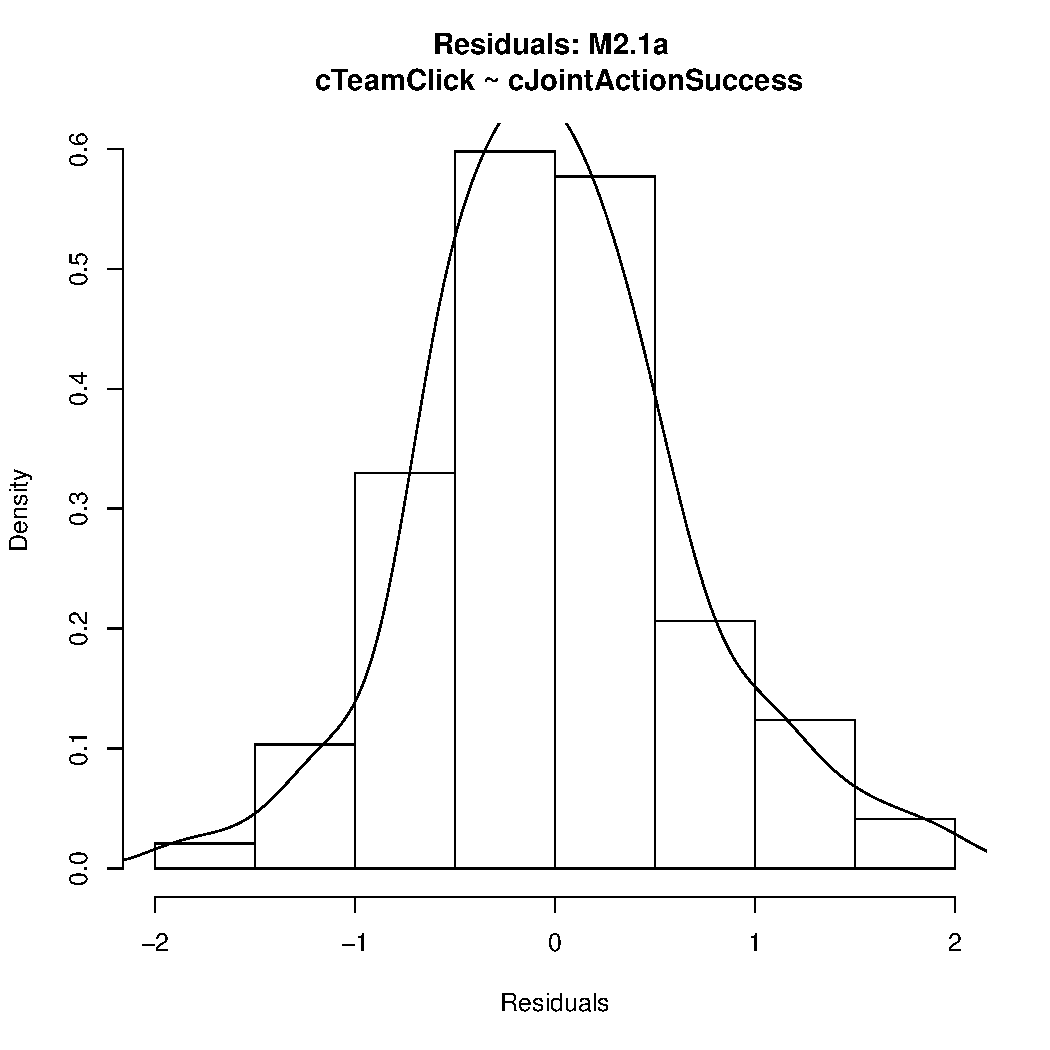
\includegraphics[scale =.4]{images/MLM21aHist.pdf}
  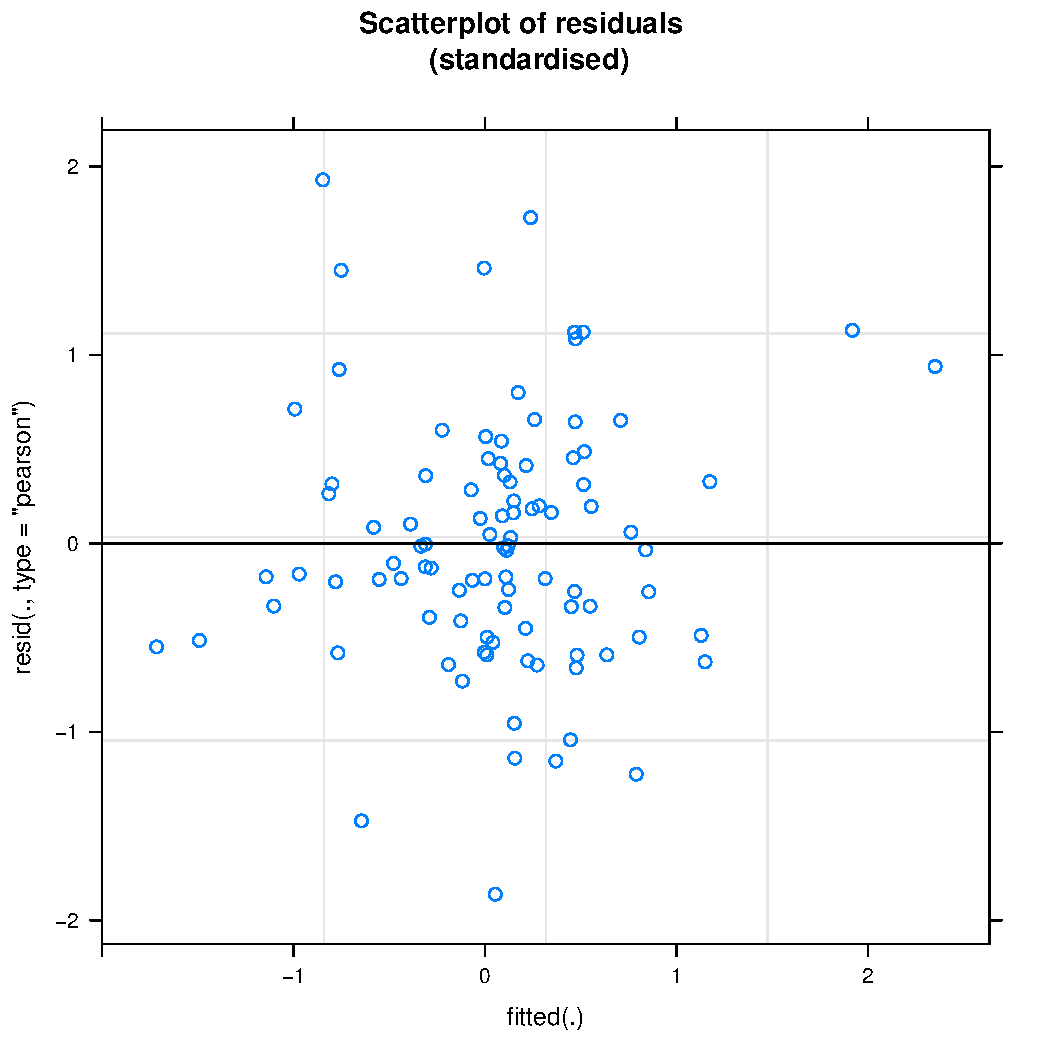
\includegraphics[scale =.4]{images/MLM21aScatter.pdf}
  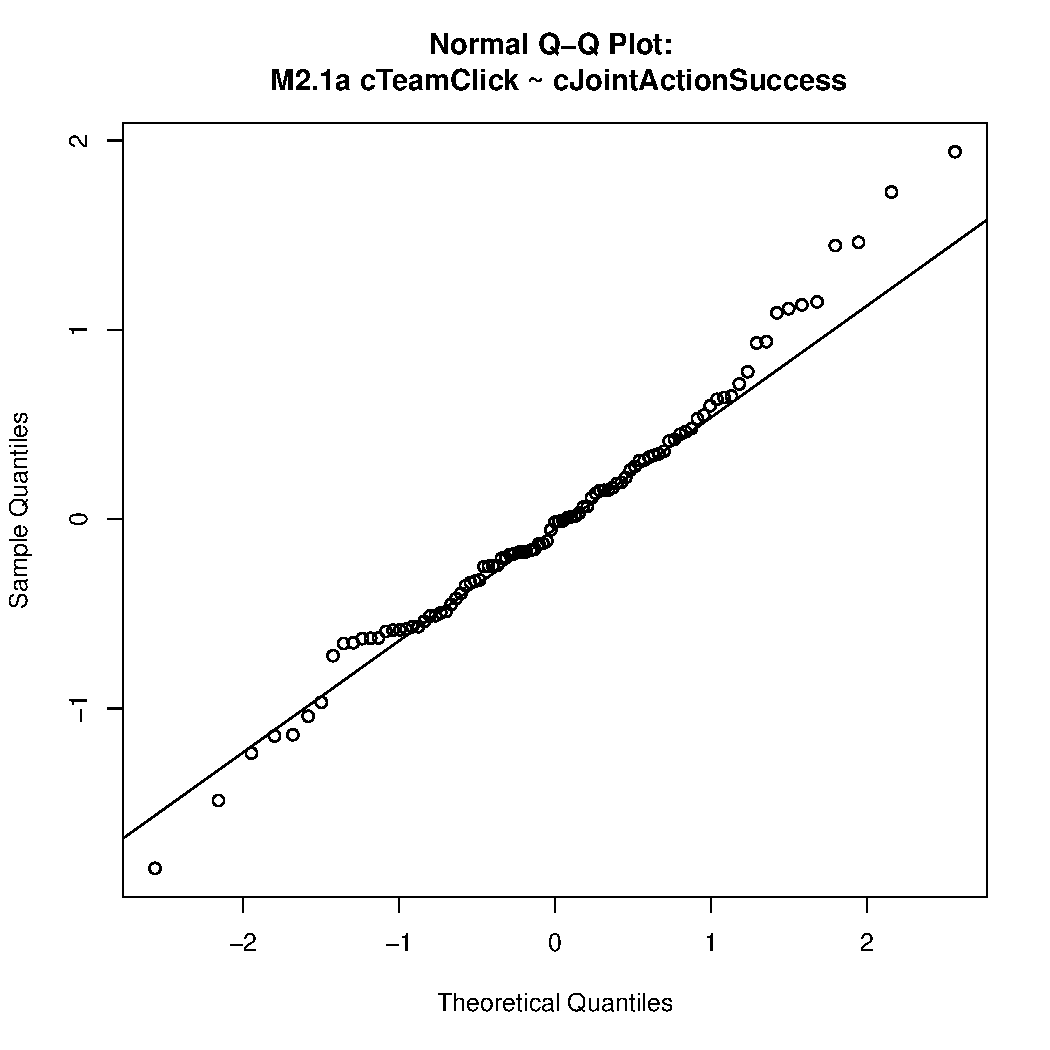
\includegraphics[scale =.4]{images/MLM21aQQNorm.pdf}
  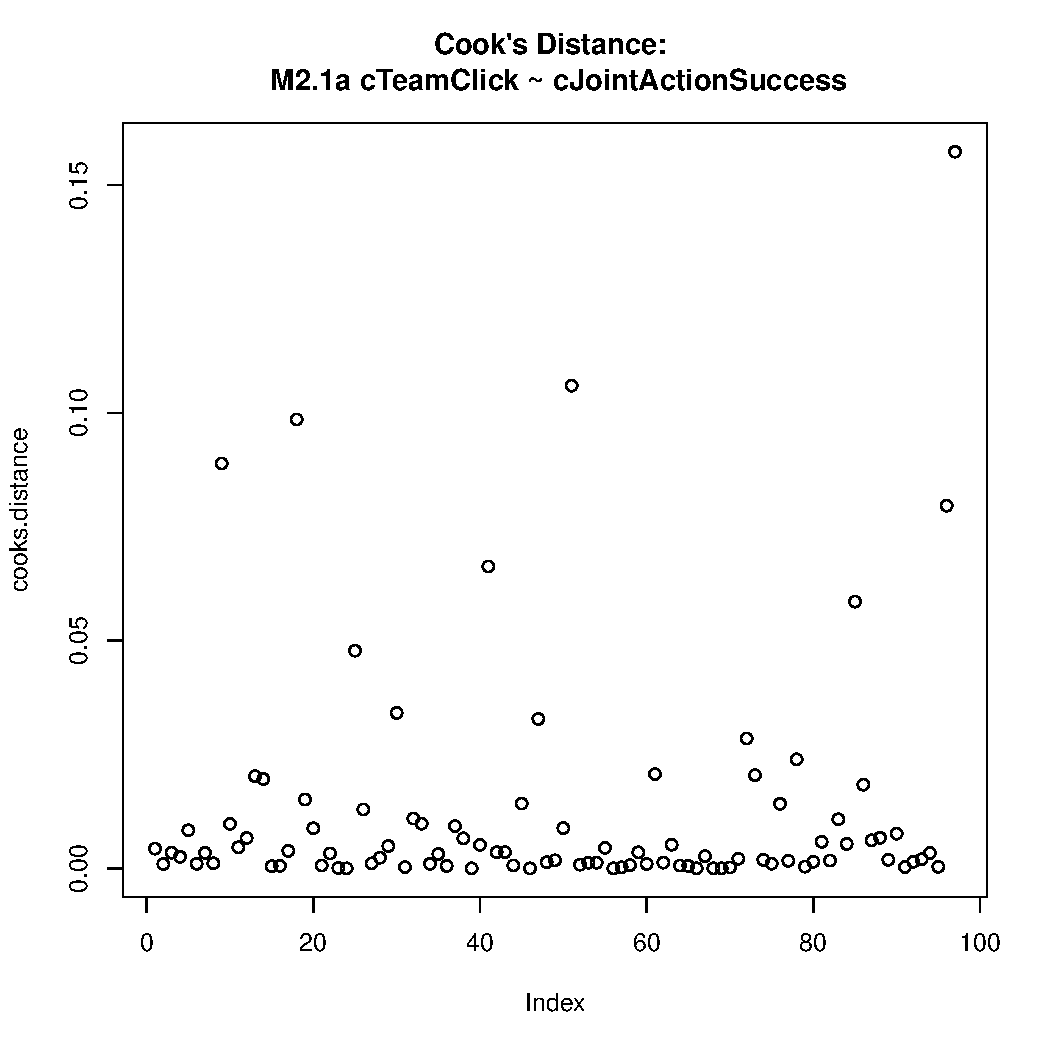
\includegraphics[scale =.4]{images/MLM21aCooksD.pdf}
  \caption{Model Assumptions: M2.1a Change in Joint Action Success predicts change in Team Click}
  \label{fig:MLM21aAssumptions}
\end{figure}





\begin{figure}[htbp]
  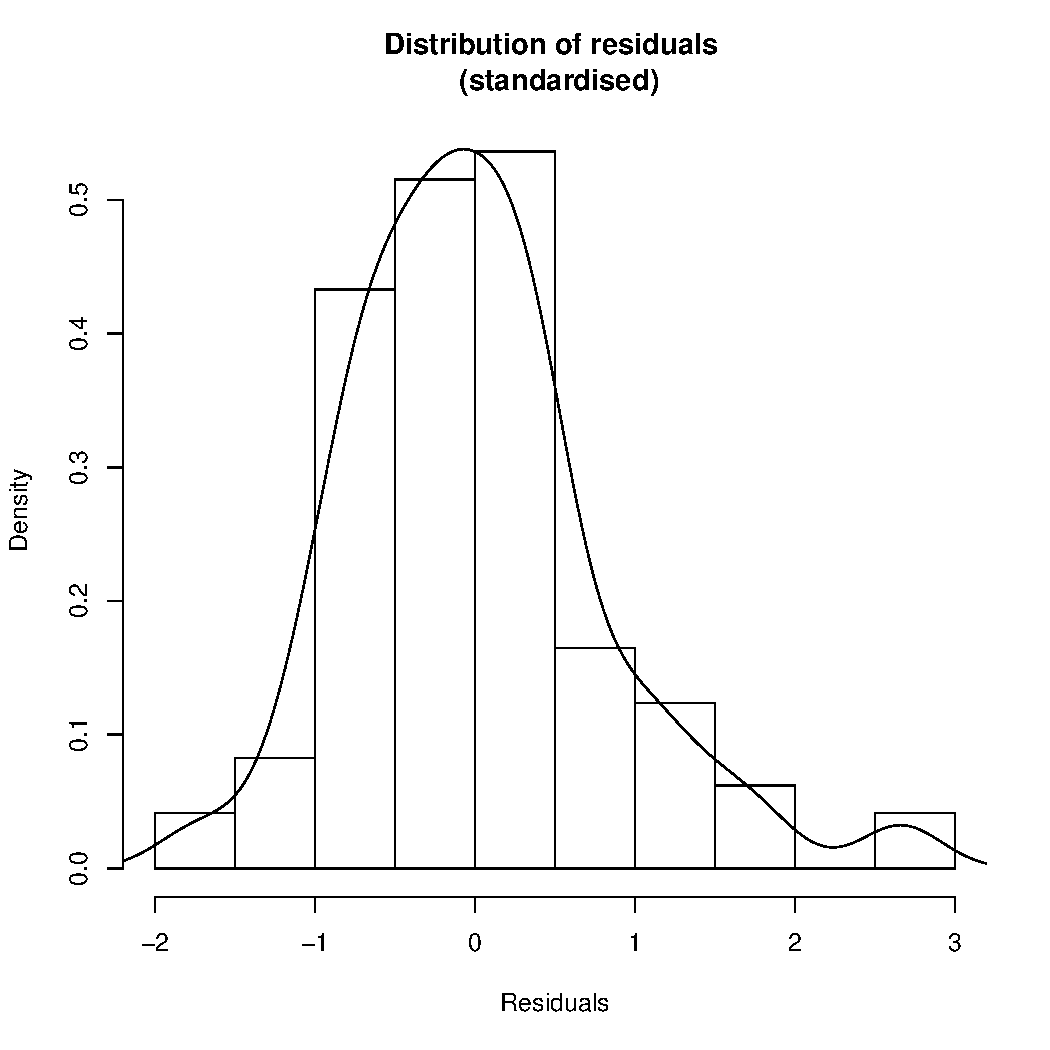
\includegraphics[scale =.4]{images/MLM21bHist.pdf}
  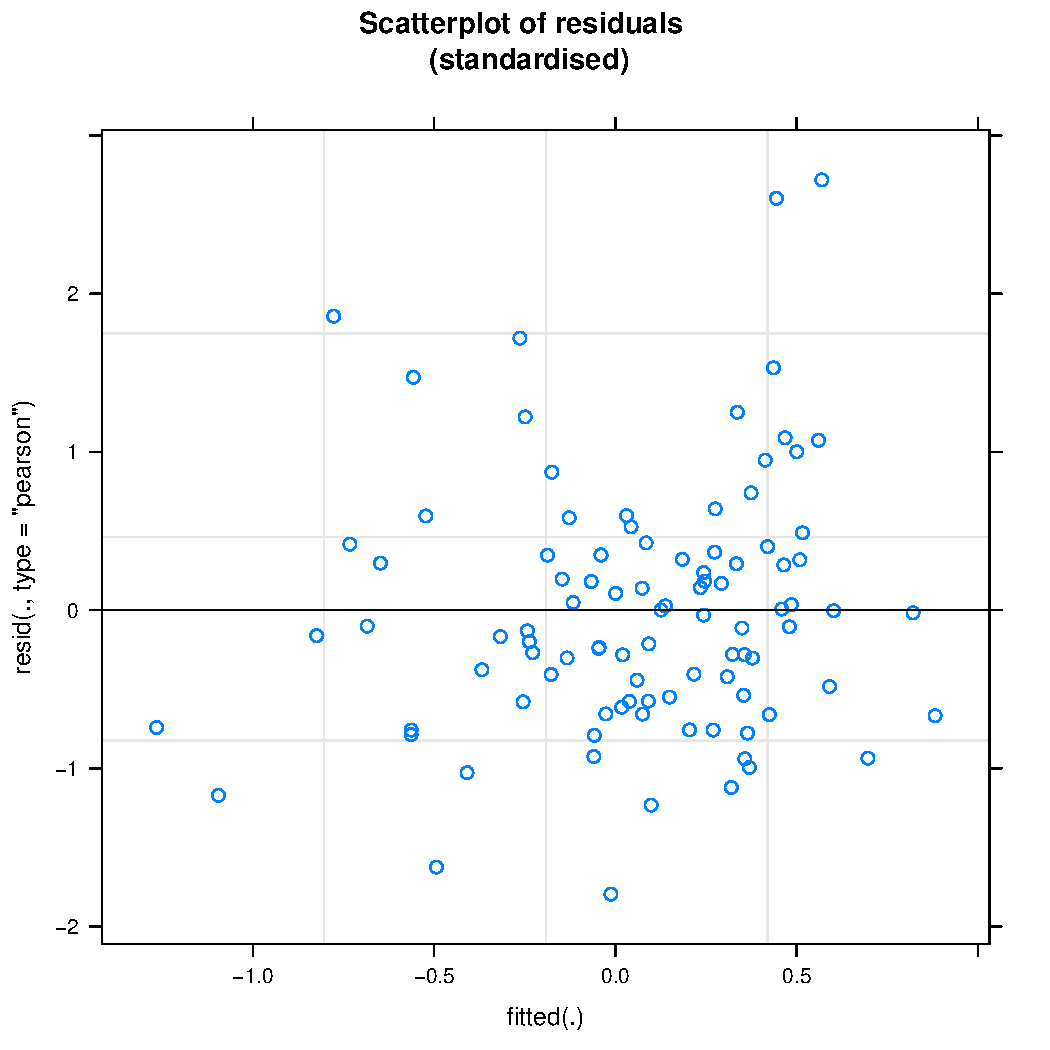
\includegraphics[scale =.4]{images/MLM21bScatter.pdf}
  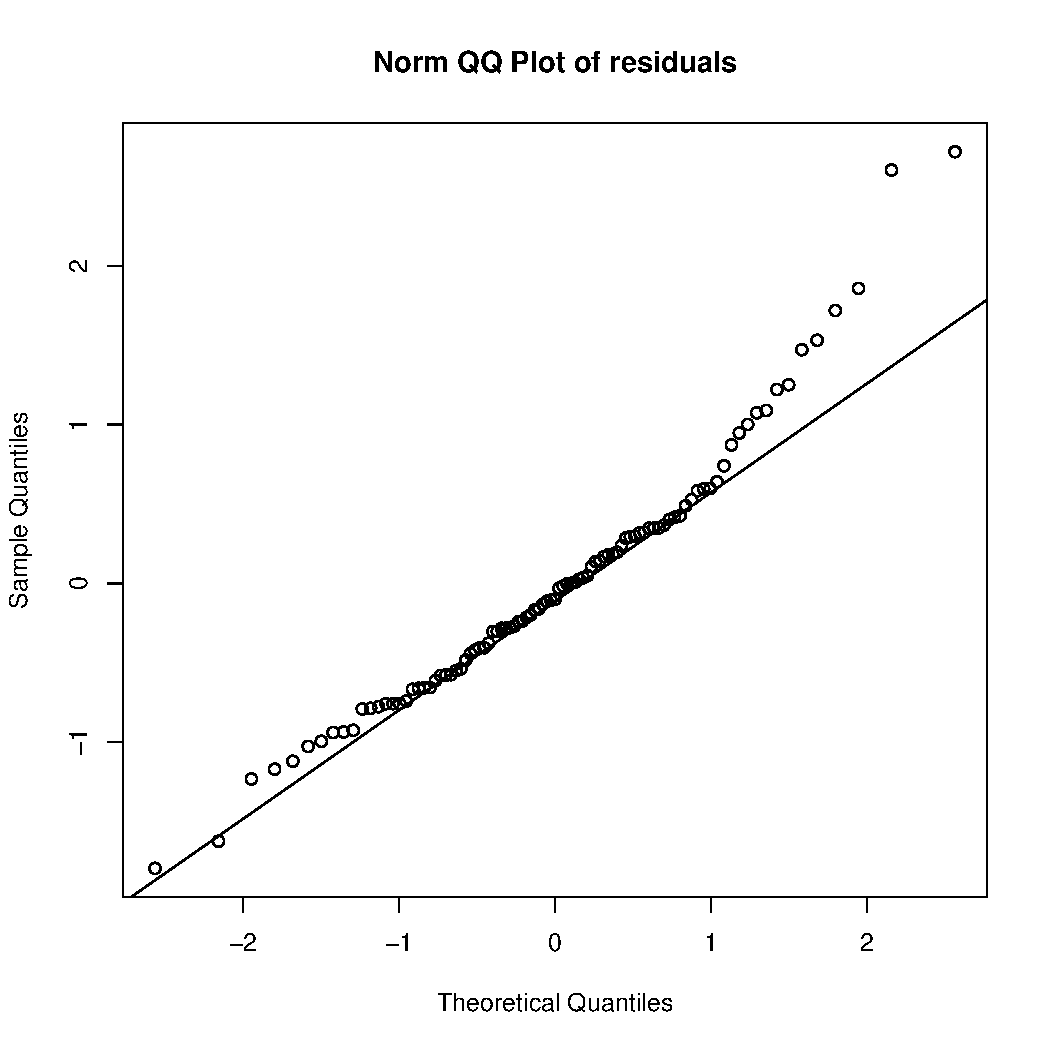
\includegraphics[scale =.4]{images/MLM21bQQNorm.pdf}
  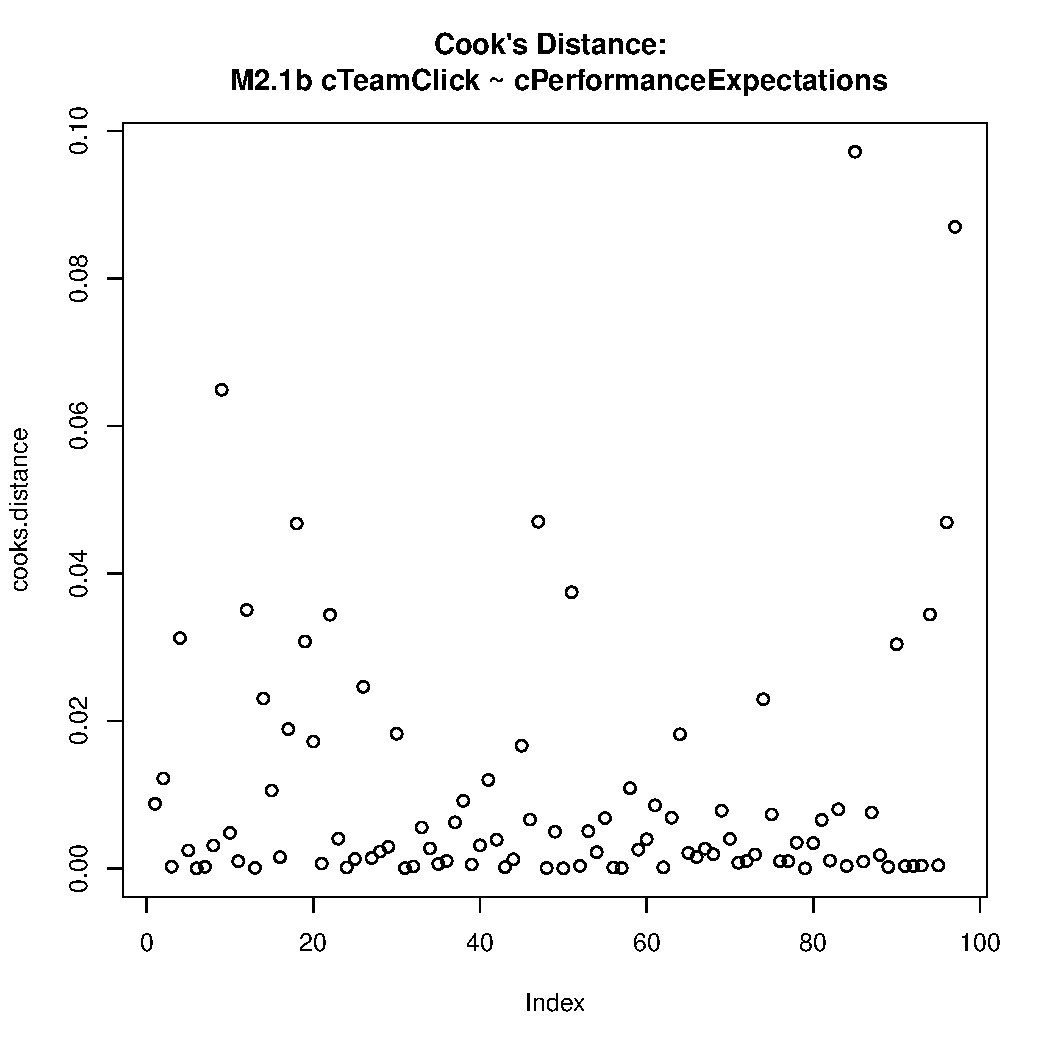
\includegraphics[scale =.4]{images/MLM21bCooksD.pdf}
  \caption{Model Assumptions: M2.1b Team Performance Expectations post-Tournament predicts change in Team Click}
  \label{fig:MLM21bAssumptions}
\end{figure}


\begin{figure}[htbp]
  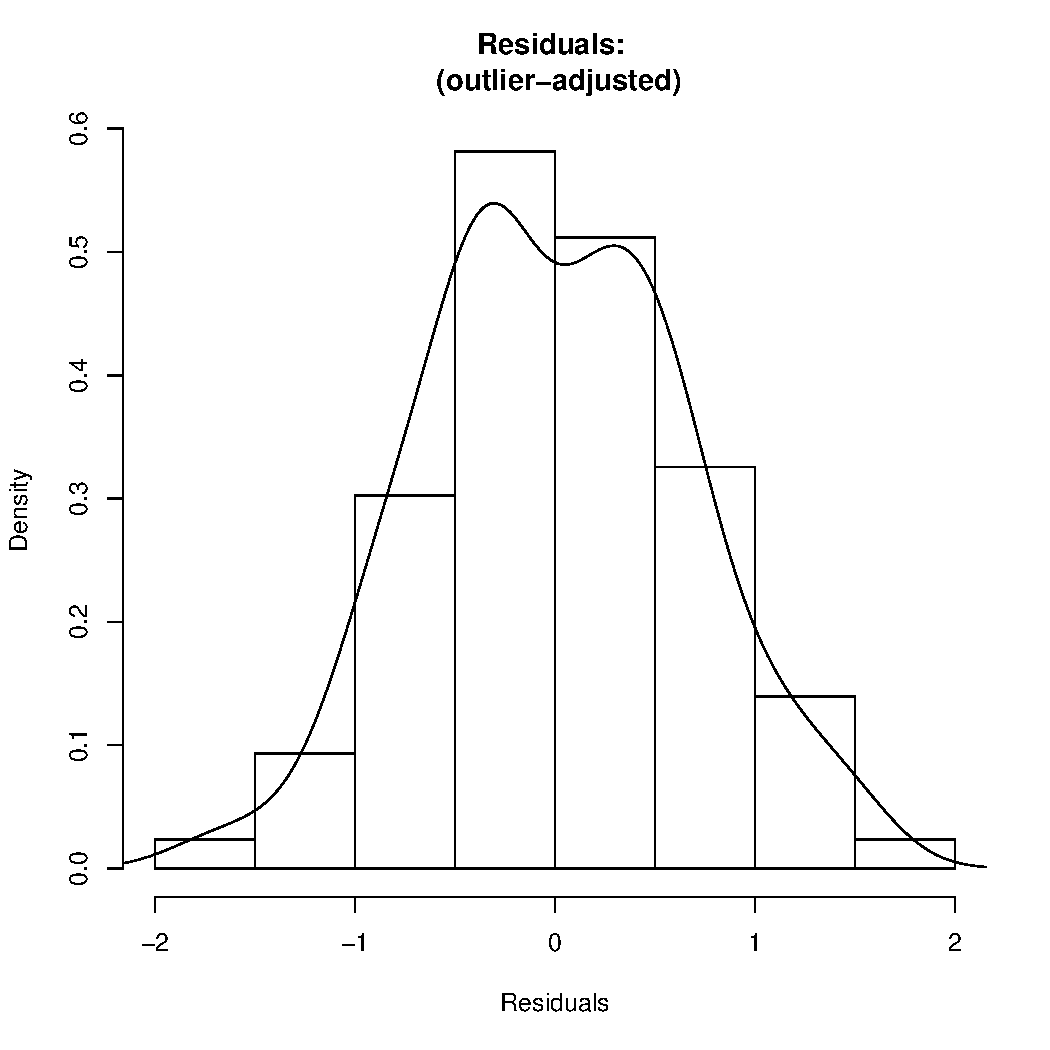
\includegraphics[scale =.4]{images/MLM21bOutHist.pdf}
  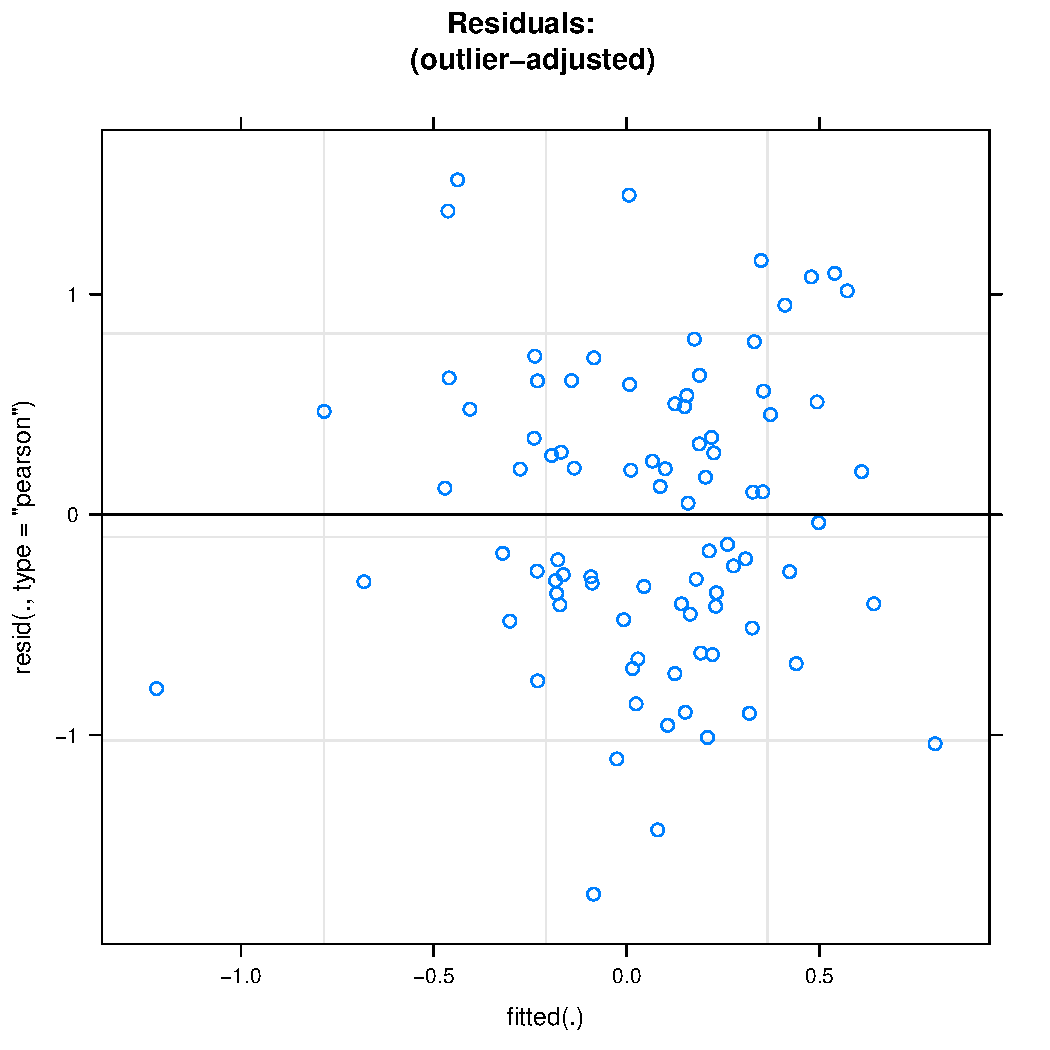
\includegraphics[scale =.4]{images/MLM21bOutScatter.pdf}
  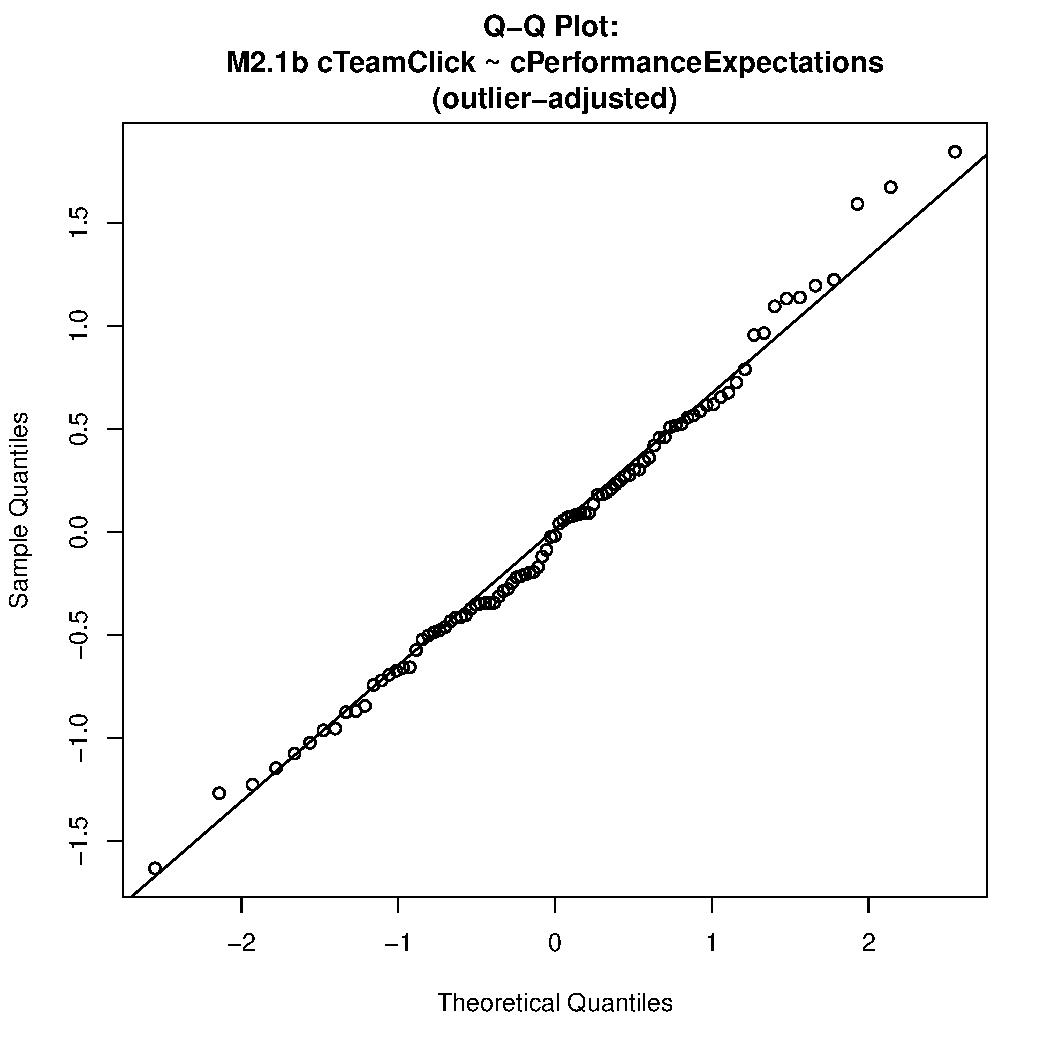
\includegraphics[scale =.4]{images/MLM21bOutQQNorm.pdf}
  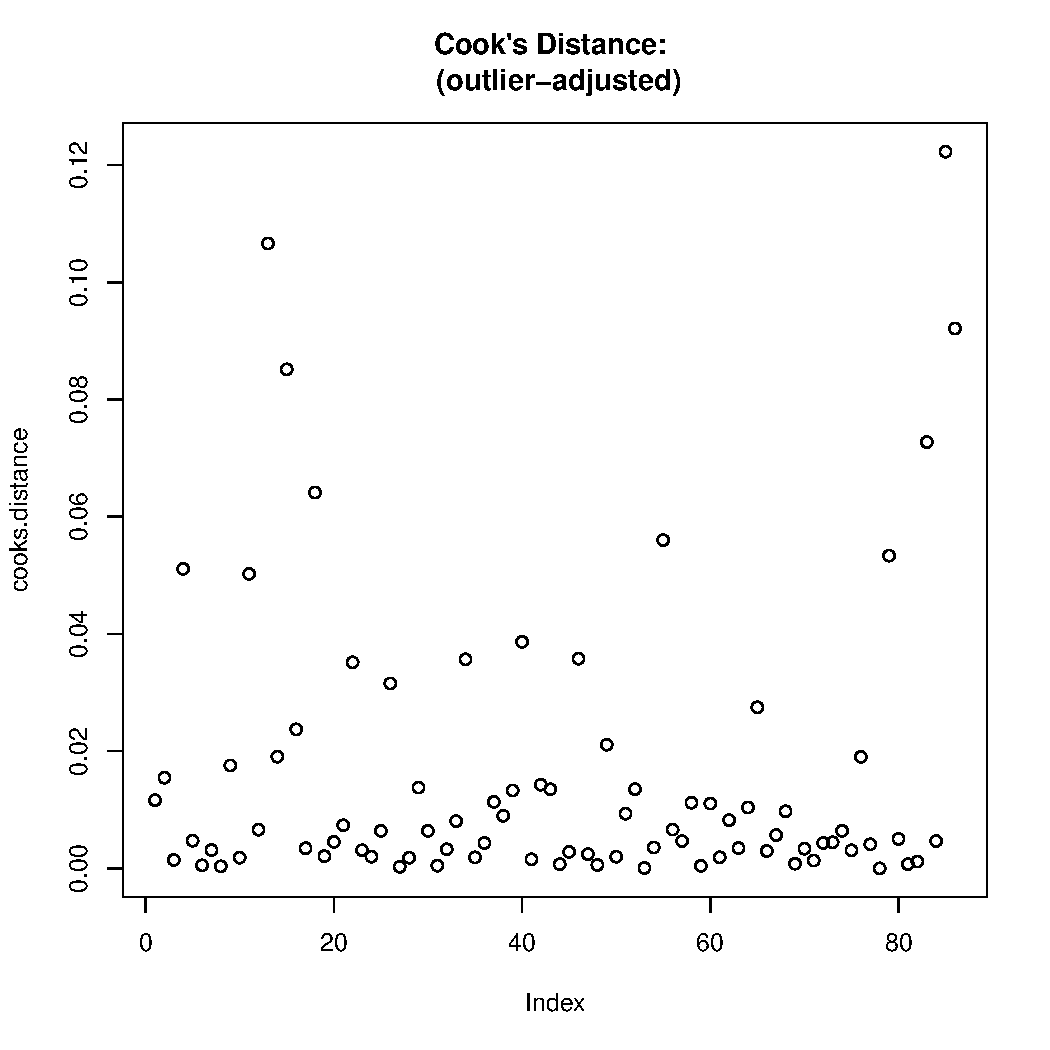
\includegraphics[scale =.4]{images/MLM21bOutCooksD.pdf}
  \caption{Model Assumptions: M2.1b Team Performance Expectations post-Tournament predicts change in Team Click (outliers removed)}
  \label{fig:MLM21bOutAssumptions}
\end{figure}



\begin{figure}[htbp]
  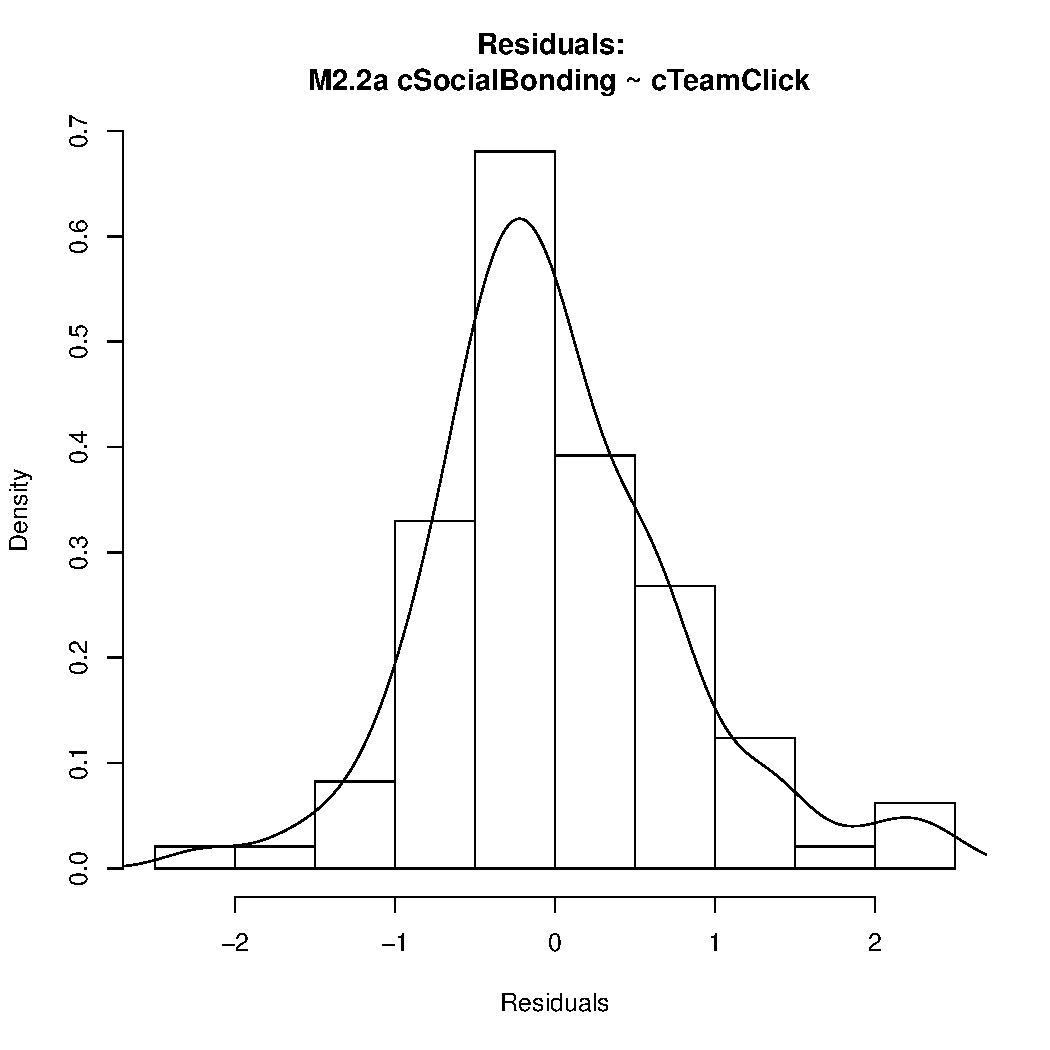
\includegraphics[scale =.4]{images/MLM22aHist.pdf}
  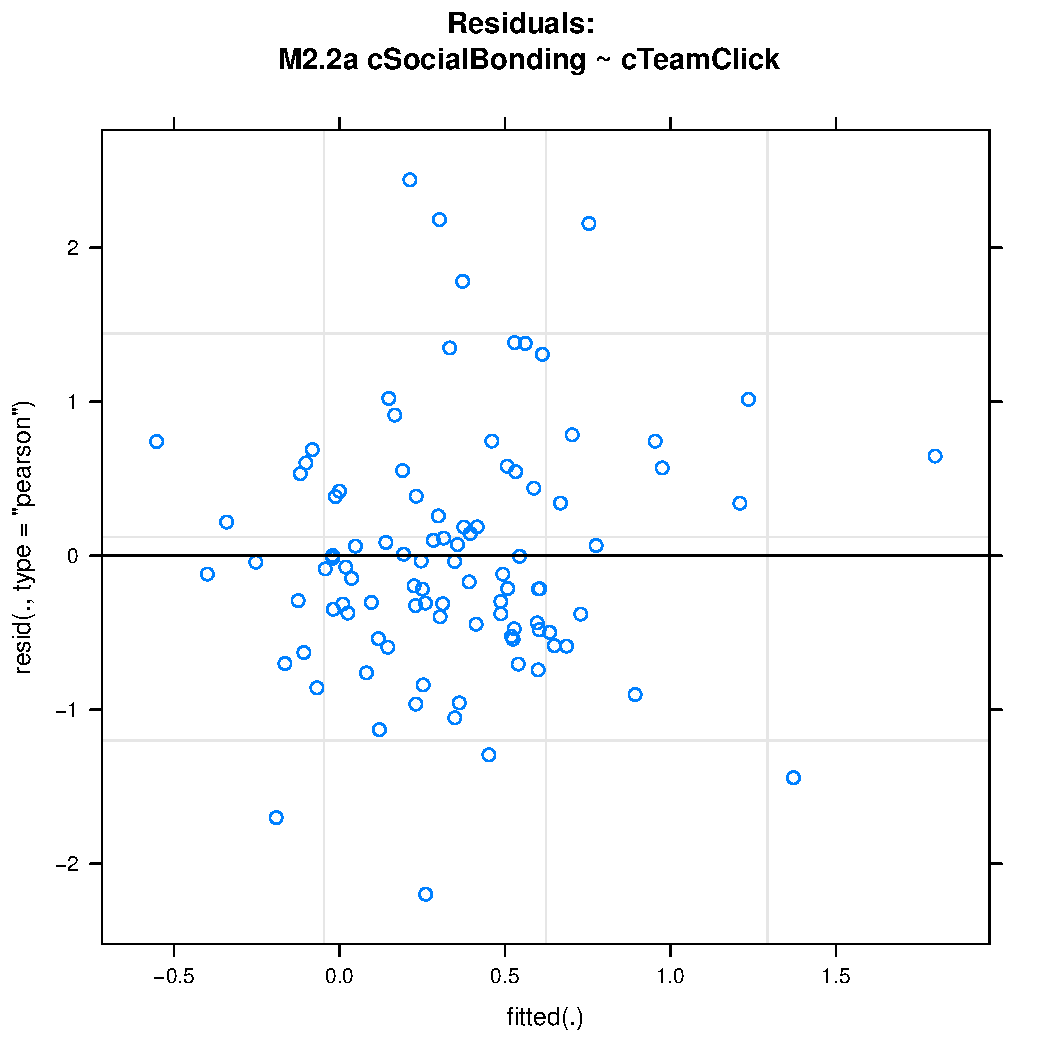
\includegraphics[scale =.4]{images/MLM22aScatter.pdf}
  \includegraphics[scale =.4]{images/MLM22aQQNorm.pdf}
  \includegraphics[scale =.4]{images/MLM22aCooksD.pdf}
  \caption{Model Assumptions: M2.2a Change in Team Click predicts change in Social Bonding}
  \label{fig:MLM22aAssumptions}
\end{figure}


\begin{figure}[htbp]
  \includegraphics[scale =.4]{images/MLM23aHist.pdf}
  \includegraphics[scale =.4]{images/MLM23aScatter.pdf}
  \includegraphics[scale =.4]{images/MLM23aQQNorm.pdf}
  \includegraphics[scale =.4]{images/MLM23aCooksD.pdf}
  \caption{Model Assumptions: M2.3a Change in Joint Action Success predicts change in Social Bonding}
  \label{fig:MLM23aAssumptions}
\end{figure}



\begin{figure}[htbp]
  \includegraphics[scale =.4]{images/MLM23aHist.pdf}
  \includegraphics[scale =.4]{images/MLM23aScatter.pdf}
  \includegraphics[scale =.4]{images/MLM23aQQNorm.pdf}
  \includegraphics[scale =.4]{images/MLM23aCooksD.pdf}
  \caption{Model Assumptions: M2.3a Change in Joint Action Success predicts change in Social Bonding}
  \label{fig:MLM23aAssumptions}
\end{figure}






\subsubsection{Additional Analysis: What predicts change in fusion to family?}
Both verbal and pictorial measures of fusion to team did not vary significantly in pre-post Tournament measures (see descriptives Table ~\ref{tab:factorsPrePostSummary}).  Interestingly, the pictorial measure of fusion to family did increase significantly between pre- and post-Tournament measurements.  Exploratory analysis was performed to investigate the possible correlates of this increase. In line with the predictions of this study, we tested whether 1) changes in perceptions of Joint Action Success, 2) Team Click, and 3) their interaction (Joint Action Success x Team Click) predicted change in fusion to family.

\myparagraph{$\Delta$Fusion Family $\sim$ $\Delta$Joint Action Success}
The first model revealed a significant effect of change in perceptions of joint-action success and change in fusion to family, $\beta = .43$ ($95\% CI =  .07, .79$), $SE = .18$, $t(6.96) = 2.34$, $p = .$, $marginal R^2 = .11$, $conditional R^2 = .14$.  The distribution of residuals indicated a poor model fit, ($W = 0.90$, $p < .00001$), due to high kurtosis ($> 2$), but not skew (.30). Given that log-transformation was not appropriate for normalising kurtosis \citep{Glass1972}, the analysis was re-run after excluding influential outliers.  The adjusted model was a much better fit, with model residuals normally distributed around zero, ($W = 0.99$, $p-value < .60$), see Table ~\ref{tab:MLM25acFusioncJointAction}. The model confirmed a significant positive relationship between change in perceptions of joint-action success and change in fusion to family, $\beta = .36$ ($95\% CI =  .19, .52$), $SE = .08$, $t() = 4.36$, $p = .$, $marginal R^2 = .32$, $conditional R^2 = .32$.


% Table created by stargazer v.5.2 by Marek Hlavac, Harvard University. E-mail: hlavac at fas.harvard.edu
% Date and time: Tue, Jun 27, 2017 - 10:42:15
\begin{table}[!htbp] \centering 
  \caption{cFusionFamily ~ jointActionSuccess} 
  \label{tab:MLM25acFusioncJointAction} 
\footnotesize 
\begin{tabular}{@{\extracolsep{5pt}}lcc} 
\\[-1.8ex]\hline 
\hline \\[-1.8ex] 
 & \multicolumn{2}{c}{\textit{Dependent variable:}} \\ 
\cline{2-3} 
\\[-1.8ex] & cFusionFamily & fusionPictorialFamilyChangeOut \\ 
 &  & outliers removed \\ 
\\[-1.8ex] & (1) & (2)\\ 
\hline \\[-1.8ex] 
 (constant) & 0.12 & $-$0.04 \\ 
  & (0.66) & (0.32) \\ 
  & & \\ 
 cJointActionSuccess & 0.43$^{**}$ & 0.50$^{***}$ \\ 
  & (0.18) & (0.10) \\ 
  & & \\ 
 cIndPerformanceSuccess & $-$0.46$^{**}$ & $-$0.01 \\ 
  & (0.20) & (0.10) \\ 
  & & \\ 
 teamPerformanceExpectations & $-$0.01 & 0.002 \\ 
  & (0.01) & (0.004) \\ 
  & & \\ 
 indPerformanceExpectations & 0.001 & $-$0.003 \\ 
  & (0.01) & (0.004) \\ 
  & & \\ 
 objectiveCompetence & 0.27 & 0.06 \\ 
  & (0.19) & (0.09) \\ 
  & & \\ 
 subjectiveCompetence & 0.06 & $-$0.0003 \\ 
  & (0.16) & (0.08) \\ 
  & & \\ 
 finalRank & 0.10 & $-$0.02 \\ 
  & (0.08) & (0.04) \\ 
  & & \\ 
 minutesTotal & $-$0.002 & 0.01 \\ 
  & (0.01) & (0.004) \\ 
  & & \\ 
\hline \\[-1.8ex] 
Marginal R-squared & .11 & .32 \\ 
Conditional R-squared & .14 & .32 \\ 
Observations & 97 & 97 \\ 
Log Likelihood & $-$173.00 & $-$104.99 \\ 
Akaike Inf. Crit. & 372.00 & 235.98 \\ 
Bayesian Inf. Crit. & 405.48 & 269.45 \\ 
\hline 
\hline \\[-1.8ex] 
\textit{Note:}  & \multicolumn{2}{r}{$^{*}$p$<$0.1; $^{**}$p$<$0.05; $^{***}$p$<$0.01} \\ 
\end{tabular} 
\end{table} 

% Table created by stargazer v.5.2 by Marek Hlavac, Harvard University. E-mail: hlavac at fas.harvard.edu
% Date and time: Tue, Jun 27, 2017 - 10:42:15
\begin{table}[!htbp] \centering 
  \caption{cFusionFamily ~ jointActionSuccess} 
  \label{tab:MLM25acFusioncJointAction} 
\footnotesize 
\begin{tabular}{@{\extracolsep{5pt}} ccc} 
\\[-1.8ex]\hline 
\hline \\[-1.8ex] 
$0.05$ & $0.01$ & $0.001$ \\ 
\hline \\[-1.8ex] 
\end{tabular} 
\end{table} 


%Need to do a multivariate regression here with family, country, team as outcomes?
\myparagraph{$\Delta$fusionFamily $\sim$ $\Delta$Team Click}

This model revealed that change in feelings of team-click was not a significant predictor of change in fusion to family, $\beta = .07$ ($95\% CI =  -.30, .44$), $SE = .19$, $t() = .38$, $p = .$, $marginal R^2 = .04$, $conditional R^2 = .07$. No other predictors in the model were statistically significant.

\myparagraph{$\Delta$fusionFamily $\sim$  $\Delta$Joint Action Success $\times$ $\Delta$Team Click}

The final model included an interaction between change in perceptions of joint-action success and change in feelings of team click as possible predictor of change in fusion to family.  Results of the model revealed that the interaction between change in perceptions of joint-action success and change in feelings of team-click was a significant positive predictor of change in fusion to family, $\beta = .22$ ($95\% CI =  .02, .41$), $SE = .10$, $t() = 2.22$, $p = .$, $marginal R^2 = .17$, $conditional R^2 = .23$. Model residuals were non-normally distributed, ($W = 0.93$, $p < .00001$).\\

This result is consistent with ethnographic findings, whereby the family unit is elevated above the team and other priorities.  This results will be considered in more depth once ethnographic analysis has also been completed.














\subsection{Analysis of post-Tournament data}
%\subsubsection{Roadmap of post-Tournament Analysis}
Analysis of the post-Tournament data proceeded by testing predictions associated with the overarching hypothesis, that higher perceptions of joint-action success would lead to higher levels of social bonding, mediated by feelings of ``team click''.

The first step was to assess whether the two variables hypothesised to be relevant to perceived joint-action success, 1) perceptions of team performance (Joint Action Success) and 2) perceptions of team performance relative to prior expectations (Team Performance Expectations), predicted feelings of team click (Team Click). Controlling for athlete perceptions of individual performance success, subjective and objective technical competence, Tournament performance measures, and variation attributable to team membership (random effect), linear mixed-effect regression models were used to test the following predictions:

\begin{description}
  \item [Prediction 1.a] Joint Action Success  $\rightarrow$ Team Click
  \item [Prediction 1.b] Team Performance Expectations $\rightarrow$ Team Click
  \item [Prediction 1.c] Joint Action Success $\rightarrow$ Team Click, moderated by Team Performance Expectations
\end{description}

Next, the relationship between team click (Team Click) and social bonding (Social Bonding) was tested, controlling for subjective and objective technical competence, Tournament performance measures, and variation attributable to team membership (random effect):

\begin{description}
  \item [Prediction 2.a] Team Click $\rightarrow$ Social Bonding
\end{description}

Following this, the direct relationships between two predictor variables of interest (Joint Action Success and Team Performance Expectations) and social bonding was tested:

\begin{description}
  \item [Prediction 3.a] Joint Action Success $\rightarrow$ Social Bonding
  \item [Prediction 3.b] Team Performance Expectations $\rightarrow$ Social Bonding
\end{description}

Finally, a mediation analysis was performed to formally test whether feelings of team click mediated a direct relationship between perceptions of joint-action success and social bonding.

\begin{description}
\item[Prediction 4.a Mediation Analysis] Joint Action Success $\rightarrow$ Team Click $\rightarrow$ Social Bonding
\item[Prediction 4.b Mediation Analysis] Team Performance Expectations $\rightarrow$ Team Click $\rightarrow$ Social Bonding
\end{description}


















\subsection{Post-Tournament Results}

\subsubsection{1.a: Joint Action Success predicts Team Click}
\subsubsection{1.b Team Performance Expectations predict Team Click}
\subsubsection{1.c Team Performance Expectations moderates the effect of Joint Action Success on team Click}

%Findings from the first collection of models generally supported predictions. Team performance factors\nobreakdashperceptions of team component performance success and team performance relative to prior expectations\nobreakdashbut not individual performance factors significantly predicted team click, when controlling for subjective and objective competence, and Tournament performance measures.  The interaction effect of joint-action success and team performance expectations violation on team click was not significant.  Additionally, the low coefficient value for the model in which teamPerformanceExpectations predicted team click was low, indicating that this result should be treated with some caution.  Taken together, however, these results provide evidence for the predictions that perceptions of joint-action success is linked to feelings of team click.  Team performance expectations do not interact with perceptions of joint action to enhance feelings of team click, but rather function independently to predict team click, with those athletes who were experienced more positive violations of expectations also reporting higher levels of team click.

\subsubsection{2.a Team Click predicts Social Bonding}
\subsubsection{3.a Joint Action Success predicts Social Bonding}
\subsubsection{3.b Team Performance Expectations predicts Social Bonding} % very small effect
\subsubsection{4.a Mediation analysis: Joint Action Success predicts Social Bonding, mediated by Team Click}
\subsubsection{4.b Mediation analysis: Team Performance Expectations predicts Social Bonding, mediated by Team Click}

%\begin{figure}[htbp]
%  \includegraphics{finalDocuments/images/MLM4aResiduals.pdf}
%  \includegraphics{finalDocuments/images/MLM4aQQNorm.pdf}
%  \includegraphics{finalDocuments/images/MLM4aResiduals.pdf}
%  \includegraphics{finalDocuments/images/MLM4aCooksD.pdf}
%  \caption{M4a Mediation Analysis}
%  \label{fig:MLM4aAssumptions}
%\end{figure}

% (Baer et al 2006: 147) One method for constructing CIs assumes normality for the sampling distributions of the estimates. Under this assumption, 95% CIs for the average indirect effect and average total effect are obtained as Alternatively, one could perform a null hypothesis test by forming the critical ratio of each estimate to its standard error and comparing the result with the critical value of the z distribution. In andthe as- sumption of normality for the sampling distributions will not hold exactly, given that aˆb ˆ is a product of normally distributed estimates (and hence will not be normal). The deviation from normality may be small enough, however, that the CIs or significance tests will still be reasonably accurate.

%An alternative method for constructing CIs that may hold promise is the Monte Carlo (MC) method of MacKinnon et al. (2004). In this approach, the sampling distribution for the effect of interest is not assumed to be normal and is instead simulated from the model estimates and their asymptotic variances and covariances (a form of parametric bootstrap- ping). For instance, to simulate the sampling distribution of the average indirect effect, one would define a multinormal distribution with means equal to a ˆ, b ˆ, and ˆ aj ,bj and covariance matrix equal to the estimated covariance matrix of these estimates. One would then take random values from this multinormal distribution and plug them into Equation 5 to compute the average indirect effect. Collecting the results over many draws provides a simulated sampling distribution for the average indirect effect. One would then obtain conidence limits for the average indirect effect by taking the

%Preacher, K. J., & Selig, J. P. (2010, July). Monte Carlo method for assessing multilevel Mediation: An interactive tool for creating confidence intervals for indirect effects in 1-1-1 multilevel models [Computer software]. Available from http://quantpsy.org/.


\subsection{Discussion of Results: post-Tournament Analysis}
The results of the post-Tournament survey responses generally support predictions concerning the relationships between perceptions of joint action success, team click and social bonding.  The relationship between team performance expectations, team click, and social bonding, however, is less convincing.  Model 1.b, in which Team Performance Expectations predicts Team Click, while statistically significant, generates a very small beta coefficient.  Model 3.b, in which the relationship between Team Performance Expectations and Social Bonding, is not robust to model assumptions, and thus compromises the validity of the mediation analysis (model 4.b).  These results could suggest that while more positive violations of team performance expectations do contribute to feelings of Team Click, they might not contribute as strongly to feelings of social bonding.

Results show that, by contrast, perceived Joint Action Success is a strong predictor of both Team Click and Social bonding. Mediation analysis indicates that Team Click fully mediates the relationship between Joint Action Success and Social Bonding.












\subsubsection{Roadmap of pre-post Tournament Analysis}
Analysis of the pre-post Tournament data proceeded in the same manner as the post-Tournament data. The hypothesised relationship between joint-action success and social bonding was broken down into component relationships. \\

First, changes in feelings of team click were analysed as a function of changes in 1) perceptions of team component performance (Joint Action Success Pre Post), 2) post-Tournament appraisal of team performance relative to prior expectations (Team Performance Expectations), and 3) the interaction between these two predictor variables.
\bigskip
\begin{description}
  \item [Prediction 2.1.a] $\Delta$Joint Action Success  $\rightarrow$  $\Delta$Team Click
  \item [Prediction 2.1.b] $\Delta$Team Performance Expectations $\rightarrow$ $\Delta$ Team Click
  \item [Prediction 2.1.c] $\Delta$Joint Action Success $\rightarrow$ $\Delta$Team Click, moderated by $\Delta$Team Performance Expectations
\end{description}

Second, the change observed in social bonding (Social Bonding Pre Post) was analysed as a function of change in feelings of team click.
\bigskip
\begin{description}
  \item [Prediction 2.2.a] $\Delta$Team Click $\rightarrow$ $\Delta$Social Bonding
\end{description}

Third, the direct relationships between predictor variables (change in perceptions of join-action success and appraisal of team performance relative to prior expectation) and change in social bonding was analysed:
\bigskip
\begin{description}
  \item [Prediction 2.3.a] $\Delta$Joint Action Success $\rightarrow$ $\Delta$Social Bonding
  \item [Prediction 2.3.b] $\Delta$Team Performance Expectations $\rightarrow$ $\Delta$Social Bonding
\end{description}

Finally, a mediation analysis was performed to formally test whether feelings of team click mediated a direct relationship between perceptions of joint-action success and social bonding.

\begin{description}
  \item[Prediction 2.4.a Mediation Analysis] $\Delta$Joint Action Success $\rightarrow$ $\Delta$Team Click $\rightarrow$ $\Delta$Social Bonding
\end{description}

\clearpage


%\subsubsection{Pre-post Tournament Descriptive Analysis}




\subsection{Analysis of pre to post-Tournament data}
The predictions of the present study were further tested through an analysis of change in variables of interest between the pre- and post-Tournament surveys. By analysing pre- and post-Tournament responses, it was possible to investigate 1) to what extent variables of interest changed during the Tournament, and 2) whether pre-post changes in variables of interest were consistent with study predictions concerning the relationship between joint-action, team click, and social bonding.  When controlling for objective measures of success and feelings concerning individual performance, could change in social bonding be explained by changes in perceptions of joint-action success and/or changes in feelings of team click?




\subsection{Model Selection}
The statistics outlined above suggested that further analysis into the relationships between changing variables was appropriate. The number of observations available in the pre-post Tournament data were insufficient to construct a mixed-effects repeated measures design in which both the intercept and slope of observations could vary according to each individual athlete nested within their given team over time.\footnote{Allowing both the intercept and slope to vary requires twice the number of observations to estimate the random effects ($2x174 = 248$), whereas the available number of observations was only 198} Alternative models for suitable for repeated measures designs, such as RM-ANOVA or ANCOVA, are also incapable of allowing each fixed factor (the regression coefficient or slope) to vary randomly according to higher level factors (individual and team), and are also unable to handle unbalanced designs (in this case, due missing data for athletes across pre- and post-Tournament measurements). As a compromise, change scores in variables of interest (individual and team performance, team click, social bonding, and fatigue) were calculated by subtracting pre- from post-Tournament scores for each athlete. The calculation of change scores reduced the complexity of the data structure down to two levels of analysis, and meant that relationships between these change variables could be modelled using a linear mixed effects regression. Change scores of relevant factors were introduced to the model as fixed effects, and their slopes and intercepts were allowed to vary according to team.

\subsection{Discussion of Results: pre- to post-Tournament Analysis}
  The results of the pre-post Tournament analysis, like the post-Tournament analysis reported above, provide support for the predictions of this study.  Increases in positive perceptions of joint-action success correlated with a larger increase in feelings of team click pre-post Tournament: athletes who experienced a positive increase in perceptions of joint-action success also reported a positive increase in feelings of team click.  Likewise, those who experienced more positive violations of team performance expectations (measured following the Tournament) also experienced a higher increase in feelings of team click pre-post Tournament.  The interaction between Joint Action Success and Team Performance Expectations, however, was not significant. Further, increases in perception of joint action success (but not team performance expectations) significantly predicted increases in feelings of social bonding before and after the Tournament.  Mediation analysis revealed that variation in team click partially mediated a direct relationship between joint action success and social bonding, however this result was only a significant trend (p = .06).  Team Performance Expectations failed to satisfactorily predict social bonding, and so was not considered in a mediation analysis


\subsection{Analysis \& results of overall Tournament data}
In the final section of analysis, evidence for a relationship between joint-action success, team click, and social bonding was assessed across the entire data set. Given that the mid-Tournament survey was truncated to accord with athlete schedules and convenience following games, variables that could be analysed across the entire tournament were limited to those that appeared in the mid-Tournament surveys. Time constraints meant that component performance was not assessed in the mid-Tournament survey, and only appraisals of overall individual and team performance relative to prior expectations were included. The mid-Tournament survey contained three team click items (Unspoken Understanding, General Atmosphere, and Click Pictorial), three social bonding items (Emotional Support, Shared Goal, and Fusion Pictorial), and three fatigue items (Fatigue, Physical Exertion, Mental Exertion). These groups of variables were all subjected to data reduction (EFA) for the purposes of analysis.



\subsubsection{Roadmap of Overall Tournament Analysis}
Analysis of the overall Tournament data proceeded in the same step-wise fashion as analyses above. First, the relationship between Team Performance Expectations and team click Team Click was tested, controlling for Tournament performance, perceptions of individual performance, and competence.

\begin{description}
  \item [Prediction 3.1.b] Team Performance Expectations $\rightarrow$ Team Click
\end{description}

Next, the relationship between Team Click and Social Bonding was tested, followed by a test of the direct relationship between Team Performance Expectations and Social Bonding:

\begin{description}
  \item [Prediction 3.2.a] Team Click $\rightarrow$ Social Bonding
  \item [Prediction 3.2.b] Team Performance Expectations $\rightarrow$ Social Bonding
\end{description}
\bigskip
Finally, a mediation analysis was conducted, in which the interaction effect of Team Performance Expectations and team click on social bonding was tested.
\bigskip
\begin{description}
\item[Prediction 3.4.a] Team Performance Expectations^*Team Click  $\rightarrow$ Social Bonding
\item[Prediction 3.4.b] Mediation Analysis: Team Performance Expectations $\rightarrow$ Team Click $\rightarrow$ Social Bonding
\end{description}
\clearpage






\subsection{Overall Tournament Results}
In the final section, the entire data set was utilised to analyse a relationship between joint-action, team click, and social bonding. As described in the previous section, items relating to performance, team click, and social bonding that were consistent across the data set were reduced to factors in order to test study predictions. The repeated measures design of this analysis made it possible to statistically account for variation in responses due to repeated sampling of the same individual athlete throughout the Tournament, and due to the fact that each athlete was member of a specific team. The following models used a three-level structure, with responses across the four time points (level 1) nested within individual athletes (level 2), who were nested within individual teams (level 3). Both the slopes and intercepts were allowed to vary for every fixed effect of the model.













%  plot() interaction






\subsubsection{Discussion of overall Tournament results}






 \subsection{Pre-post Tournament differences in latent factors}
 Following data reduction, paired samples t-tests were used to compare Pre- and Post-Tournament measures of extracted factors relating to team and individual performance, team click, social bonding, and fatigue. Results are displayed in Table ~\ref{}.  Mean difference between athlete scores of team component performance (Team Performance Components Pre Post) did not vary significantly from pre- to post-Tournament, $M = -.06 (-.30  .18)$, $t(98)= -.48, p = .63$, nor did team click, $M = .06 (-.12, .25)$, $t(98)= .69, p = .49$. Athlete mean differences in perceptions of components of individual performance (Individual Performance Success Pre Post) significantly decreased following the Tournament, $M = -.28 (-.47, -.10)$, $t(98)= -2.99, p = .003$, suggesting that athletes were on average more critical of their individual performance than their team performance at the completion of the Tournament.

 Tests revealed that the there was a significant difference in athlete reports of Social Bonding between pre- and Post-Tournament surveys, $M = .34(.16, .52)$, $t(98)= 3.73, p = .0003$; Athletes' feelings of bonding on average increased from pre- to post-Tournament.  Average ratings of Fatigue also significantly increased from measurement following athletes' second game on Day 1 to ratings following the Tournament, $M =  .77(.55, .99)$, $t(116)= 7.03, p < .0001$ (see Table ~\ref{tab:factorsPrePostSummary}).

 \newgeometry{margin=0.5cm} % modify this if you need even more space
 \begin{landscape}
 
% Table created by stargazer v.5.2 by Marek Hlavac, Harvard University. E-mail: hlavac at fas.harvard.edu
% Date and time: Sat, Jun 03, 2017 - 17:41:41
\begin{table}[!htbp] \centering 
  \caption{factors change pre-post Tournament} 
  \label{} 
\footnotesize 
\begin{tabular}{@{\extracolsep{5pt}} cccccccccc} 
\\[-1.8ex]\hline 
\hline \\[-1.8ex] 
 & Variable & Mean.pre & SD.pre & Mean.post & SD.post & MeanDiffernece & MeanPairedDifference & t-test & p-value \\ 
\hline \\[-1.8ex] 
1 & teamPerformanceFactorPrePost & $$-$0.01$ & $1.04$ & $0.01$ & $0.88$ & $0.01$ & $$-$0.06$ & $$-$0.48$ & $0.63$ \\ 
2 & indPerformanceFactorPrePost & $0.12$ & $0.95$ & $$-$0.13$ & $0.93$ & $$-$0.25$ & $$-$0.28$ & $$-$2.99$ & $0.004$ \\ 
3 & clickFactorPrePost & $$-$0.04$ & $0.98$ & $0.04$ & $0.85$ & $0.09$ & $0.06$ & $0.69$ & $0.84$ \\ 
4 & bondingFactorPrePost & $$-$0.18$ & $1.03$ & $0.19$ & $0.71$ & $0.37$ & $0.34$ & $3.74$ & $0.0003$ \\ 
5 & fatigueFactorPrePost & $$-$0.29$ & $1.01$ & $0.40$ & $0.65$ & $0.68$ & $0.77$ & $7.03$ & $0$ \\ 
\hline \\[-1.8ex] 
\end{tabular} 
\end{table} 

  \end{landscape}
 \restoregeometry








 \section{Analysis of study predictions}


 \subsection{Prediction 1: More positive perceptions of team performance predict higher levels of Team Click}

 \subsubsection{Prediction 1.a: Perceptions of success in components of joint action predict Team Click}




 \myparagraph{Post-Tournament Survey}

 \begin{align*}
   Team Click =  & Team Performance Components\\
             & + Individual Performance Components \\
             & + Objective Competence + Subjective Competence\\
             & + TournamentPerformanceMeasures \\
 \end{align*}

 
\begin{table}
\begin{center}
\begin{tabular}{l c c c }
\toprule
 & Intercept & Main effect & Controls \\
\midrule
(constant)                                                & $-0.04$  & $0.02$                & $-0.55$               \\
                                                          & $(0.15)$ & $(0.07)$              & $(0.37)$              \\
Team Performance Components                               &          & $\mathbf{0.65}^{***}$ & $\mathbf{0.66}^{***}$ \\
                                                          &          & $(0.10)$              & $(0.11)$              \\
Ind Performance Components                                &          &                       & $-0.04$               \\
                                                          &          &                       & $(0.09)$              \\
Objective Competence                                      &          &                       & $0.05$                \\
                                                          &          &                       & $(0.08)$              \\
Subjective Competence                                     &          &                       & $0.11$                \\
                                                          &          &                       & $(0.07)$              \\
Final Rank                                                &          &                       & $0.03$                \\
                                                          &          &                       & $(0.04)$              \\
Minutes Total                                             &          &                       & $0.00$                \\
                                                          &          &                       & $(0.00)$              \\
Points Total                                              &          &                       & $0.00$                \\
                                                          &          &                       & $(0.01)$              \\
Fatigue                                                   &          &                       & $0.10$                \\
                                                          &          &                       & $(0.08)$              \\
Extraverted                                               &          &                       & $0.03$                \\
                                                          &          &                       & $(0.05)$              \\
\midrule
AIC                                                       & 299.06   & 237.51                & 211.70                \\
BIC                                                       & 307.37   & 254.14                & 247.75                \\
Log Likelihood                                            & -146.53  & -112.76               & -91.85                \\
Num. obs.                                                 & 118      & 118                   & 97                    \\
\bottomrule
\multicolumn{4}{l}{\scriptsize{Coefficients with $p < 0.05$ in \textbf{bold}. Marginal $R^2 = .56$, Conditional $R^2 = .61$}}
\end{tabular}
\caption{Prediction 1: Team Performance Components predicts Team Click in the Post-Tournament survey data.}
\label{tab:MLM1aJointActionSuccessClick}
\end{center}
\end{table}






\bigskip


 \begin{figure}[htbp]
   \centering
 \includegraphics[scale=.5]{images/jasClickBasicXY.pdf}
   \caption{Team Performance Components predicts Team Click (n = 118)}
   \label{fig:jasClickBasicXY}
 \end{figure}


 \begin{figure}[htbp]
   \centering
 \includegraphics[scale = .5]{images/jasClickModelSlope}
   \caption{Team Performance Components predicts Team Click. The blue slope is the original line of best fit, the red slope has been adjusted according to the predictions of the linear model}
   \label{fig:jasClickModelSLope}
 \end{figure}



 \myparagraph{Pre- to Post-Tournament}


 \begin{figure}[htbp]
   \centering
 \includegraphics[scale=.5]{images/jasClickDeltaBasicXY}
   \caption{Changes in Team Performance Components predicts changes in Team Click. The blue slope is the original line of best fit, the red slope has been adjusted according to the predictions of the linear model}
   \label{fig:jasClickDeltaBasicXY}
 \end{figure}

 
% Table created by stargazer v.5.2 by Marek Hlavac, Harvard University. E-mail: hlavac at fas.harvard.edu
% Date and time: Tue, Jun 27, 2017 - 09:10:21
\begin{table}[!htbp] \centering 
  \caption{cTeamClick ~ cJointActionSuccess} 
  \label{tab:MLM21aJointActionSuccesscClick} 
\begin{tabular}{@{\extracolsep{5pt}}lccc} 
\\[-1.8ex]\hline 
\hline \\[-1.8ex] 
 & \multicolumn{3}{c}{\textit{Dependent variable:}} \\ 
\cline{2-4} 
\\[-1.8ex] & \multicolumn{3}{c}{cTeamClick} \\ 
\\[-1.8ex] & (1) & (2) & (3)\\ 
\hline \\[-1.8ex] 
 (constant) & 0.10 & 0.10 & $-$0.10 \\ 
  & (0.13) & (0.08) & (0.28) \\ 
  & & & \\ 
 cJointActionSuccess &  & 0.47$^{***}$ & 0.52$^{***}$ \\ 
  &  & (0.08) & (0.09) \\ 
  & & & \\ 
 cIndPerformanceSuccess &  &  & $-$0.04 \\ 
  &  &  & (0.09) \\ 
  & & & \\ 
 objectiveCompetence &  &  & 0.03 \\ 
  &  &  & (0.09) \\ 
  & & & \\ 
 subjectiveCompetence &  &  & $-$0.01 \\ 
  &  &  & (0.08) \\ 
  & & & \\ 
 finalRank &  &  & $-$0.02 \\ 
  &  &  & (0.04) \\ 
  & & & \\ 
 minutesTotal &  &  & 0.004 \\ 
  &  &  & (0.004) \\ 
  & & & \\ 
 pointsTotal &  &  & 0.01 \\ 
  &  &  & (0.01) \\ 
  & & & \\ 
\hline \\[-1.8ex] 
Marginal R-squared &  &  & .40 \\ 
Conditional R-squared &  &  & .47 \\ 
Observations & 99 & 99 & 97 \\ 
Log Likelihood & $-$130.59 & $-$107.75 & $-$104.44 \\ 
Akaike Inf. Crit. & 267.19 & 227.50 & 232.88 \\ 
Bayesian Inf. Crit. & 274.97 & 243.07 & 263.77 \\ 
\hline 
\hline \\[-1.8ex] 
\textit{Note:}  & \multicolumn{3}{r}{$^{*}$p$<$0.05; $^{**}$p$<$0.01; $^{***}$p$<$0.001} \\ 
\end{tabular} 
\end{table} 


 \begin{figure}[htbp]
   \centering
 \includegraphics[scale=.5]{images/jasClickDeltaModelSlope}
   \caption{Change in Team Performance Components predicts change in Team Click. The blue slope is the original line of best fit, the red slope has been adjusted according to the predictions of the linear model.}
   \label{fig:jasClickDeltaModelSLope}
 \end{figure}






 \subsubsection{Prediction 1.b: Team Performance Expectations predicts Team Click}


 \myparagraph{Post-Tournament}


 \begin{align*}
   Team Click =  & Team Performance Expectations \\
             &+ Individual Performance Expectations \\
             &+ Objective Competence + Subjective Competence \\
             &+ Tournament performance measures \\
 \end{align*}


 \begin{figure}[htbp]
   \centering
 \includegraphics[scale=.5]{images/teamPerfClickBasicXY.pdf}
   \caption{Team Performance Expectations predicts Team Click (n = 118)}
   \label{fig:teamPerfClickBasicXY}
 \end{figure}


   
\begin{table}
\begin{center}
\begin{tabular}{l c c c }
\toprule
 & Intercept & Main effect & Controls \\
\midrule
(constant)                                 & $-0.04$  & $-0.00$               & $\mathbf{-0.79}^{*}$  \\
                                           & $(0.15)$ & $(0.09)$              & $(0.40)$              \\
Team Performance Vs Expectations           &          & $\mathbf{0.50}^{***}$ & $\mathbf{0.51}^{***}$ \\
                                           &          & $(0.11)$              & $(0.12)$              \\
Ind Performance Vs Expectations            &          &                       & $0.02$                \\
                                           &          &                       & $(0.08)$              \\
Objective Competence                       &          &                       & $0.02$                \\
                                           &          &                       & $(0.08)$              \\
Subjective Competence                      &          &                       & $0.12$                \\
                                           &          &                       & $(0.07)$              \\
Final Rank                                 &          &                       & $\mathbf{0.09}^{*}$   \\
                                           &          &                       & $(0.05)$              \\
Minutes Total                              &          &                       & $-0.00$               \\
                                           &          &                       & $(0.00)$              \\
Points Total                               &          &                       & $0.00$                \\
                                           &          &                       & $(0.01)$              \\
Fatigue                                    &          &                       & $\mathbf{0.18}^{*}$   \\
                                           &          &                       & $(0.09)$              \\
Extraverted                                &          &                       & $0.06$                \\
                                           &          &                       & $(0.05)$              \\
\midrule
AIC                                        & 299.06   & 268.43                & 228.63                \\
BIC                                        & 307.37   & 285.06                & 264.68                \\
Log Likelihood                             & -146.53  & -128.22               & -100.32               \\
Num. obs.                                  & 118      & 118                   & 97                    \\
Num. groups: team                          & 15       & 15                    & 14                    \\
\bottomrule
\multicolumn{4}{l}{\scriptsize{Coefficients with $p < 0.05$ in \textbf{bold}. Marginal $R^2 = .40$, Conditional $R^2 = .56$}}
\end{tabular}
\caption{Prediction 5: Team Performance Vs Expectations predicts Team Click in the Post-Tournament survey data (n = 97).}
\label{tab:MLM1bteamExpectationsClick}
\end{center}
\end{table}


   \begin{figure}[htbp]
     \centering
   \includegraphics[scale=.5]{images/teamPerfClickModelSlope.pdf}
     \caption{Team Performance Expectations predicts Team Click. The blue slope is the original line of best fit, the red slope has been adjusted according to the predictions of the linear model.}
     \label{fig:teamPerfClickModelSlope}
   \end{figure}



   \myparagraph{Pre- to Post-Tournament change}
 Given that the item measuring Athlete perceptions of overall team performance in the Pre-Tournament survey was not framed in terms of expectation violation (but instead in terms of more or less ``good'' or ``poor''), it was not possible to directly compare the Pre- and Post-Tournament measures.  Instead, the Post-Tournament measure of Team Performance Expectation violation was analysed in terms of its relationship to a change in feelings of team click between Pre- and Post-Tournament measurements. Did more positive violations of team performance expectations following the Tournament predict an increase in feelings of team click? A scatterplot depicting the relationship between Team Performance Expectations and change in Team Click is shown in Figure ~\ref{fig:teamPerfClickDeltaBasicXY}. The plot indicates a positive (albeit less pronounced) relationship between Team Performance Expectations and change in Team Click.
     %\subsubsection{2.1.b $\Delta$Team Click $\sim$ Team Performance Expectations}

 The relationship between team performance relative to prior expectations (recorded Post-Tournament) and Team Click was analysed using a linear mixed effects model. The model revealed a significant positive relationship between Team Performance Expectations and change in Team Click,  $\beta = .27$ ($95\% CI =  .05, .49$), $SE = .11$, $t(32.97) = 2.36$, $p = .02$, $marginal R^2 = .12$, $conditional R^2 = .22$, indicating that athletes who were more positive about their appraisals of team performance following the Tournament on average experienced an increase in feelings of team click.

 Examination of model residuals revealed that they were not normally distributed around zero ($W = .95, p = .001$), due to positive skew ($.85$) (see Appendix Figure ~\ref{fig:MLM21bAssumptions}).  Non-normally distributed residuals are problematic as they may influence the model's ability to generate accurate parameter estimates . Two data manipulation techniques were considered in order to normalise residuals and therefore preserve the estimates of the model: exclusion of outliers and transformation of the outcome variable.  Transformation of the outcome variables was the preferred method over outlier exclusion, due to the cost involved in removing observations that may be of potential theoretical relevance to the scientific investigation \citep{Rousseeuw2011}. Nonetheless, for this first phase of analysis, both outlier exclusion and transformation manipulations of the data were performed and reported.

 Log-transformation of the outcome variable did not markedly improve the non-normality of residuals, ($Shapiro-Wilk = .96, p = .008$).  Instead, exclusion of outliers according to Tukey's method (observations above and below 1.5x the Inter Quartile Range (IQR), see \citep{Tukey1977}) improved the model fit such that residuals were normally distributed, ($Shapiro-Wilk = .99, p = .72$), and individual cases had low influence on the model (Cook's Distances all $< .10$, see Appendix Figure ~\ref{fig:MLM21bOutAssumptions}).
 The adjusted model supported the original significant positive effect of Team Performance Expectations on Team Click, $\beta = .36$ ($95\% CI =  .16, .55$), $SE = .10$, $t(9.78) = 3.66$, $p < .01$, $marginal R^2 = .16$, $conditional R^2 = .55$.
 See Appendix ~\ref{app8:tournamentSurvey} Table ~\ref{tab:MLM21bOutLogComparison} for a comparison of adjusted models. These results confirm the prediction that those who experience more positive violations around team performance also experience an higher levels of Team Click---shown in this case by an increase in feelings of Team Click between Pre- and Post-Tournament measurements.  The slope of the adjusted model is included in the scatterplot of figure ~\ref{fig:teamPerfClickDeltaModelSlope} purposes of comparison

 %The adjusted model also revealed a significant negative effect of violations of expectations around \textit{individual} performance on team click, $\beta = -.008 (95\% CI =  -.01, .001), SE = .004, t(91.79) = -2.28, p = .03$,  which could suggest that athletes who experienced more positive violations about their own performance did not feel the team click as strongly.

     
% Table created by stargazer v.5.2 by Marek Hlavac, Harvard University. E-mail: hlavac at fas.harvard.edu
% Date and time: Tue, Jun 27, 2017 - 09:21:13
\begin{table}[!htbp] \centering 
  \caption{M2.1b cTeamClick ~ cPerformanceExpectations} 
  \label{tab:MLM21bcTeamPerfExpcClick} 
\begin{tabular}{@{\extracolsep{5pt}}lccc} 
\\[-1.8ex]\hline 
\hline \\[-1.8ex] 
 & \multicolumn{3}{c}{\textit{Dependent variable:}} \\ 
\cline{2-4} 
\\[-1.8ex] & \multicolumn{3}{c}{cTeamClick} \\ 
\\[-1.8ex] & (1) & (2) & (3)\\ 
\hline \\[-1.8ex] 
 (constant) & 0.10 & $-$0.57 & $-$0.64 \\ 
  & (0.13) & (0.30) & (0.44) \\ 
  & & & \\ 
 cTeamPerformanceExpectations &  & 0.01$^{*}$ & 0.01$^{*}$ \\ 
  &  & (0.004) & (0.005) \\ 
  & & & \\ 
 cIndPerformanceExpectations &  &  & $-$0.003 \\ 
  &  &  & (0.004) \\ 
  & & & \\ 
 objectiveCompetence &  &  & $-$0.13 \\ 
  &  &  & (0.11) \\ 
  & & & \\ 
 subjectiveCompetence &  &  & $-$0.16 \\ 
  &  &  & (0.09) \\ 
  & & & \\ 
 finalRank &  &  & 0.02 \\ 
  &  &  & (0.06) \\ 
  & & & \\ 
 minutesTotal &  &  & 0.003 \\ 
  &  &  & (0.005) \\ 
  & & & \\ 
 pointsTotal &  &  & 0.003 \\ 
  &  &  & (0.01) \\ 
  & & & \\ 
\hline \\[-1.8ex] 
Marginal R-squared &  &  & .40 \\ 
Conditional R-squared &  &  & .47 \\ 
Observations & 99 & 99 & 97 \\ 
Log Likelihood & $-$130.59 & $-$127.00 & $-$123.15 \\ 
Akaike Inf. Crit. & 267.19 & 266.01 & 270.30 \\ 
Bayesian Inf. Crit. & 274.97 & 281.58 & 301.20 \\ 
\hline 
\hline \\[-1.8ex] 
\textit{Note:}  & \multicolumn{3}{r}{$^{*}$p$<$0.05; $^{**}$p$<$0.01; $^{***}$p$<$0.001} \\ 
\end{tabular} 
\end{table} 

     
\begin{table}
\begin{center}
\begin{tabular}{l c c c }
\toprule
 & Controls & Log-adjusted & Outliers removed \\
\midrule
(constant)                                 & $0.33$               & $\mathbf{1.27}^{***}$ & $0.40$                \\
                                           & $(0.51)$             & $(0.16)$              & $(0.39)$              \\
Team Performance Vs Expectations           & $\mathbf{0.30}^{**}$ & $\mathbf{0.09}^{*}$   & $\mathbf{0.32}^{***}$ \\
                                           & $(0.11)$             & $(0.04)$              & $(0.08)$              \\
Ind Performance Vs Expectations            & $-0.10$              & $-0.03$               & $\mathbf{-0.22}^{**}$ \\
                                           & $(0.10)$             & $(0.03)$              & $(0.08)$              \\
Objective Competence                       & $-0.15$              & $-0.05$               & $0.03$                \\
                                           & $(0.12)$             & $(0.04)$              & $(0.10)$              \\
Subjective Competence                      & $-0.15$              & $-0.05$               & $-0.03$               \\
                                           & $(0.09)$             & $(0.03)$              & $(0.08)$              \\
Final Rank                                 & $-0.01$              & $-0.00$               & $-0.08$               \\
                                           & $(0.06)$             & $(0.02)$              & $(0.04)$              \\
Minutes Total                              & $0.00$               & $0.00$                & $-0.00$               \\
                                           & $(0.01)$             & $(0.00)$              & $(0.00)$              \\
Points Total                               & $0.00$               & $0.00$                & $0.01$                \\
                                           & $(0.01)$             & $(0.00)$              & $(0.01)$              \\
Fatigue                                    & $-0.08$              & $-0.00$               & $-0.07$               \\
                                           & $(0.11)$             & $(0.04)$              & $(0.09)$              \\
Extraverted                                & $-0.06$              & $-0.02$               & $0.01$                \\
                                           & $(0.07)$             & $(0.02)$              & $(0.05)$              \\
\midrule
AIC                                        & 253.92               & 50.47                 & 200.30                \\
BIC                                        & 288.92               & 85.47                 & 234.66                \\
Log Likelihood                             & -112.96              & -11.23                & -86.15                \\
Num. obs.                                  & 90                   & 90                    & 86                    \\
Num. groups: team                          & 13                   & 13                    & 13                    \\

\bottomrule
\multicolumn{4}{l}{\scriptsize{Coefficients with $p < 0.05$ in \textbf{bold}. Effect size of model excluding outliers: Marginal $R^2 = .17$, Conditional $R^2 = .20$}}
\end{tabular}
\caption{Prediction 2: Team Click Change predicts Social Bonding Change in the Post-Tournament survey data (n = 90).}
\label{tab:MLM21bOutLogComparison}
\end{center}
\end{table}



     \begin{figure}[htbp]
       \centering
     \includegraphics[scale=.5]{images/teamPerfClickDeltaModelSlope.pdf}
       \caption{Team Performance Expectations predicts change in Team Click. The blue slope is the original line of best fit, the red slope has been adjusted according to the predictions of the linear model}
       \label{fig:teamPerfClickDeltaModelSlope}
     \end{figure}




     %Low values for both of these regression coefficients...
   \myparagraph{Overall Tournament}

 \begin{figure}[htbp]
   \centering
 \includegraphics[scale=.5]{images/teamPerfClickOverallBasicXY.pdf}
   \caption{Team Performance Expectations predicts Team Click in Overall Tournament subset}
   \label{fig:teamPerfClickOverallBasicXY}
 \end{figure}

        \begin{align*}
          Team Click =  & Team Performance Expectations  \\
                    &+ Individual Performance Expectations   \\
                    &+ Objective Competence + Subjective Competence \\
                    &+ TournamentPerformanceMeasures  \\
        \end{align*}

      \bigskip

 
    
\begin{table}
\begin{center}
\begin{tabular}{l c c c }
\toprule
 & Intercept & Main effect & Controls \\
\midrule
(constant)                                                        & $-0.00$  & $-0.06$               & $-0.12$               \\
                                                                  & $(0.04)$ & $(0.03)$              & $(0.21)$              \\
Team Performance Vs Expectations                                  &          & $\mathbf{0.74}^{***}$ & $\mathbf{0.72}^{***}$ \\
                                                                  &          & $(0.03)$              & $(0.05)$              \\
Ind Performance Vs Expectations                                   &          &                       & $\mathbf{0.12}^{**}$  \\
                                                                  &          &                       & $(0.04)$              \\
Objective Competence                                              &          &                       & $0.04$                \\
                                                                  &          &                       & $(0.04)$              \\
Subjective Competence                                             &          &                       & $0.07$                \\
                                                                  &          &                       & $(0.04)$              \\
Final Rank                                                        &          &                       & $-0.00$               \\
                                                                  &          &                       & $(0.02)$              \\
Minutes Total                                                     &          &                       & $-0.00$               \\
                                                                  &          &                       & $(0.00)$              \\
Points Total                                                      &          &                       & $0.00$                \\
                                                                  &          &                       & $(0.00)$              \\
Fatigue                                                           &          &                       & $0.00$                \\
                                                                  &          &                       & $(0.00)$              \\
Extraverted                                                       &          &                       & $0.01$                \\
                                                                  &          &                       & $(0.03)$              \\
\midrule
AIC                                                               & 1552.70  & 842.67                & 602.59                \\
BIC                                                               & 1570.04  & 879.53                & 665.89                \\
Log Likelihood                                                    & -772.35  & -412.33               & -284.30               \\
Num. obs.                                                         & 564      & 444                   & 306                   \\
\bottomrule
\multicolumn{4}{l}{\scriptsize{Coefficients with $p < 0.05$ in \textbf{bold}. Marginal $R^2 = .63$, Conditional $R^2 = .69$}}
\end{tabular}
\caption{Prediction 1: Team Performance Vs Expectations predicts Team Click in the Overall Tournament survey data (n = 90).}
\label{tab:MLM31ateamPerfClickTournament}
\end{center}
\end{table}



    \begin{figure}[htbp]
      \centering
    \includegraphics[scale=.5]{images/teamPerfClickOverallBasicXY.pdf}
      \caption{Team Performance Expectations predicts Team Click in Overall Tournament subset. The blue slope is the original line of best fit, the red slope has been adjusted according to the predictions of the linear model}
      \label{fig:teamPerfClickOverallModelSlope}
    \end{figure}

 \myparagraph{Prediction 1.b: Summary of results}
 Results from the analysis of Prediction 1.b suggest that following the Tournament, more positive violation of expectations surrounding team performance correlate with higher levels of self-reported team click.  In addition, more positive violations of expectations following the Tournament are associated with an increase in feelings of Team Click between Pre- and Post-Tournament surveys, suggesting that athletes who perceived an increase in success of components of team performance also experienced an increase in feelings of team click.  Finally, the positive relationship between Overall Tournament measures of team performance expectations and team click was also significant.




 \subsection{Prediction 1.c: Team Performance Components predicts Team Click, moderated by Team Performance Expectations}

 If both perceptions of success and positive violations of team performance expectations predict team click, do these two predictors interact to predict team click?  Is team click higher for individuals whose perceived success in joint action was also a more positive violation of performance expectation?  This possibility was tested by including the interaction term (Team Performance Components $\times$ Team Performance Expectations) in the LMER models used for the Post-Tournament and Pre- to Post-Tournament subsets as follows:


     \begin{align*}
       Team Click =  & Team Performance Components \times Team Performance Expectations \\
                 &+ Individual Performance Components \\
                 &+ Individual Performance Expectations \\
                 &+ Objective Competence + Subjective Competence  \\
                 &+ Tournament performance measures \\
     \end{align*}

   \bigskip

   \subsubsection{post-Tournamnet}
   In the case of the Post-Tournament subset, the inclusion of the interaction term failed to improve upon the fit of the previous model, judging by the relative goodness of fit, $AIC(1.c) = 217.91$ compared to $AIC(1.a) = 209.48$, $SD = .52 $, $\chi^2(18, N = 97) = 3.56$, $ p =.74$.
   Results revealed that the interaction between Team Performance Components and Team Performance Expectations was not significant, $\beta = .002$ ($95\% CI =  -.0062, .0063$), $SE = .08$, $t(39.7) = .026$, $p = .98$, $marginal R^2 = .56$, $conditional R^2 = .65$ (see Appendix ~\ref{app8:tournamentSurvey}, Table ~\ref{tab:MLM1cPerformanceClickInteraction}).


   %\textit{See appendix A for details about model assumptions}.
   %\newpage
   %\ [scale =.4]{../images/MLM1cHist.pdf}
   %\includegraphics[scale =.4]{../images/MLM1cScatter.pdf}
   %\includegraphics[scale =.4]{../images/MLM1cQQNorm.pdf}
   %\includegraphics[scale =.4]{../images/MLM1cCooksD.pdf}

   %\textit{problem here: increase in marginal and conditional R^2 values, perhaps due to adding additional variables into the model}
   %The interaction did not improve the model fit,
   %Nor did adding teamPerformance7 on its own into the model...
   %But an interaction alone was significant

   \subsubsection{Pre- to Post-Tournament change}
   %\subsubsection{2.1.c $\Delta$Team Click $\sim$ $\Delta$Team Performance Components$\times$ Team Performance Expectations}
   Introduction of the interaction effect of change in perceptions of joint action success and expectations around team performance on change in Team Click was not significant, $\beta = .004$ ($95\% CI =  -.002, .01$), $SE = .003$, $t(30.14) = 1.42$, $p = .17$, $marginal R^2 = .40$, $conditional R^2 = .49$, and failed to improve the model fit, $\chi^2 = 2.72$, $ p = .44$ (see Table ~\ref{tab:MLM21ccTeamPerfExpcClickInt}).  This result indicates that the extent to which team performance violations were more or less positive did not have an additive effect on the positive relationship between perceptions of Team Performance Components and Team Click.

   
\begin{table}
\begin{center}
\begin{tabular}{l c c c }
\toprule
 & Intercept & Main effect & Controls \\
\midrule
(constant)                                     & $\mathbf{0.34}^{***}$ & $\mathbf{0.31}^{***}$ & $0.29$               \\
                                               & $(0.09)$              & $(0.08)$              & $(0.46)$             \\
Team Click Change                              &                       & $\mathbf{0.39}^{***}$ & $\mathbf{0.37}^{**}$ \\
                                               &                       & $(0.11)$              & $(0.14)$             \\
Objective Competence                           &                       &                       & $0.08$               \\
                                               &                       &                       & $(0.10)$             \\
Subjective Competence                          &                       &                       & $0.01$               \\
                                               &                       &                       & $(0.09)$             \\
Final Rank                                     &                       &                       & $0.00$               \\
                                               &                       &                       & $(0.05)$             \\
Minutes Total                                  &                       &                       & $0.01$               \\
                                               &                       &                       & $(0.00)$             \\
Points Total                                   &                       &                       & $0.00$               \\
                                               &                       &                       & $(0.01)$             \\
Fatigue                                        &                       &                       & $-0.09$              \\
                                               &                       &                       & $(0.10)$             \\
Extraverted                                    &                       &                       & $-0.03$              \\
                                               &                       &                       & $(0.06)$             \\
\midrule
AIC                                            & 265.55                & 256.54                & 241.81               \\
BIC                                            & 273.34                & 272.11                & 274.31               \\
Log Likelihood                                 & -129.78               & -122.27               & -107.90              \\
Num. obs.                                      & 99                    & 99                    & 90                   \\
Num. groups: team                              & 14                    & 14                    & 13                   \\
\bottomrule
\multicolumn{4}{l}{\scriptsize{Coefficients with $p < 0.05$ in \textbf{bold}. Marginal $R^2 = .17$, Conditional $R^2 = .23$}}
\end{tabular}
\caption{Prediction 2: Team Click Change predicts Social Bonding Change in the Post-Tournament survey data (n = 90).}
\label{tab:MLM22acClickcBonding}
\end{center}
\end{table}


   %Exclusion of outliers according to Tukey's method (observations above and below 1.5 \times Inter Quartile Range (IQR)) appeared to improve the model fit, $\beta = .25$ ($95\% CI =  .11, .48$), $SE = .10$, $t(6.58) = 3.06$, $p < .02$, $marginal R^2 = .18$, $conditional R^2 = .25$. Model residuals were normally distributed, ($Shapiro-Wilk = .98, p = .14$),

 %\subsubsection{1.c Overall Tournament}
 %    NA
 \myparagraph{Prediction 1.c: Summary of results}
 Results from the analysis of Prediction 1.c fail to provide evidence for an interaction effect of Team Performance Components and Team Performance Expectations on social bonding.  These results suggest that the extent to which overall team performance is experienced as a violation of prior expectations does not have an additive effect on the relationship between perceptions of success in joint action and feelings of team click.

















 \subsection{Prediction 2: Team Click predicts Social Bonding}

     \begin{align*}
       Social Bonding   =& Team Click\\
                       &+ Objective Competence + Subjective Competence  \\
                       &+ Tournament performance measures \\
     \end{align*}

   \bigskip


   \myparagraph{Post-Tournament}

 \begin{figure}[htbp]
   \centering
 \includegraphics[scale=.5]{images/clickBondBasicXY.pdf}
   \caption{Team Click predicts Social Bonding in Post-Tournament survey data}
   \label{fig:clickBondBasicXY}
 \end{figure}

   
% Table created by stargazer v.5.2 by Marek Hlavac, Harvard University. E-mail: hlavac at fas.harvard.edu
% Date and time: Mon, Jun 26, 2017 - 20:48:41
\begin{table}[!htbp] \centering 
  \caption{socialBonding = teamClick} 
  \label{tab:MLM2aTeamClickBonding} 
\begin{tabular}{@{\extracolsep{5pt}}lccc} 
\\[-1.8ex]\hline 
\hline \\[-1.8ex] 
 & \multicolumn{3}{c}{\textit{Dependent variable:}} \\ 
\cline{2-4} 
\\[-1.8ex] & \multicolumn{3}{c}{socialBonding} \\ 
\\[-1.8ex] & (1) & (2) & (3)\\ 
\hline \\[-1.8ex] 
 (constant) & $-$0.01 & $-$0.0002 & 0.21 \\ 
  & (0.10) & (0.07) & (0.27) \\ 
  & & & \\ 
 teamClick &  & 0.64$^{***}$ & 0.67$^{***}$ \\ 
  &  & (0.08) & (0.08) \\ 
  & & & \\ 
 objectiveCompetence &  &  & 0.04 \\ 
  &  &  & (0.08) \\ 
  & & & \\ 
 subjectiveCompetence &  &  & 0.12 \\ 
  &  &  & (0.07) \\ 
  & & & \\ 
 finalRank &  &  & $-$0.01 \\ 
  &  &  & (0.04) \\ 
  & & & \\ 
 minutesTotal &  &  & $-$0.003 \\ 
  &  &  & (0.004) \\ 
  & & & \\ 
 pointsTotal &  &  & $-$0.002 \\ 
  &  &  & (0.01) \\ 
  & & & \\ 
\hline \\[-1.8ex] 
Marginal R-squared &  &  & .49 \\ 
Conditional R-squared &  &  & .51 \\ 
Observations & 118 & 118 & 97 \\ 
Log Likelihood & $-$151.95 & $-$118.76 & $-$97.75 \\ 
Akaike Inf. Crit. & 309.90 & 249.53 & 217.50 \\ 
Bayesian Inf. Crit. & 318.21 & 266.15 & 245.82 \\ 
\hline 
\hline \\[-1.8ex] 
\textit{Note:}  & \multicolumn{3}{r}{$^{*}$p$<$0.05; $^{**}$p$<$0.01; $^{***}$p$<$0.001} \\ 
\end{tabular} 
\end{table} 


   \begin{figure}[htbp]
     \centering
   \includegraphics[scale=.5]{images/clickBondModelSlope.pdf}
     \caption{Team Click predicts Social Bonding in Post-Tournament survey data. The blue slope is the original line of best fit, the red slope has been adjusted according to the predictions of the linear model.}
     \label{fig:clickBondModelSlope}
   \end{figure}



   \myparagraph{Pre- to Post-Tournament change}
   %\subsubsection{2.2.a $\Delta$Social Bonding$\sim$ $\Delta$Team

     \begin{figure}[htbp]
       \centering
     \includegraphics[scale=.5]{images/clickBondDeltaBasicXY.pdf}
       \caption{Change in Team Click predicts Change in Social Bonding}
       \label{fig:clickBondDeltaBasicXY}
     \end{figure}


   \begin{figure}[htbp]
     \centering
   \includegraphics[scale=.5]{images/clickBondDeltaModelSlope.pdf}
     \caption{Change in Team Click predicts change in Social Bonding in the Pre- to Post-Tournament subset of survey data. The blue slope is the original line of best fit, the red slope has been adjusted according to the predictions of the linear model.}
     \label{fig:clickBondDeltaModelSlope}
   \end{figure}


 \myparagraph{Overall Tournament}
   %\subsubsection{3.2.a Social Bonding $\sim$ Team Click}

         \begin{figure}[htbp]
           \centering
         \includegraphics[scale=.5]{images/clickBondOverallBasicXY.pdf}
           \caption{Change in Team Click predicts Change in Social Bonding}
           \label{fig:clickBondOverallBasicXY}
         \end{figure}


    
% Table created by stargazer v.5.2 by Marek Hlavac, Harvard University. E-mail: hlavac at fas.harvard.edu
% Date and time: Thu, Sep 14, 2017 - 09:39:55
\begin{table}[!htbp] \centering 
  \caption{bondingTournament ~ teamClickTournament} 
  \label{tab:MLM31bclickBondingTournament} 
\footnotesize 
\begin{tabular}{@{\extracolsep{5pt}}lccc} 
\\[-1.8ex]\hline 
\hline \\[-1.8ex] 
 & \multicolumn{3}{c}{\textit{Dependent variable:}} \\ 
\cline{2-4} 
\\[-1.8ex] & (1) & (2) & (3)\\ 
\hline \\[-1.8ex] 
 (constant) & $-$0.00 & $-$1.46$^{***}$ & $-$1.59$^{***}$ \\ 
  & (0.04) & (0.08) & (0.15) \\ 
  & & & \\ 
 teamPerformanceExpectations &  & 0.02$^{***}$ & 0.02$^{***}$ \\ 
  &  & (0.001) & (0.001) \\ 
  & & & \\ 
 indPerformanceExpectations &  &  & 0.004$^{**}$ \\ 
  &  &  & (0.002) \\ 
  & & & \\ 
 objectiveCompetence &  &  & 0.02 \\ 
  &  &  & (0.04) \\ 
  & & & \\ 
 subjectiveCompetence &  &  & 0.08$^{*}$ \\ 
  &  &  & (0.04) \\ 
  & & & \\ 
 finalRank &  &  & $-$0.0002 \\ 
  &  &  & (0.02) \\ 
  & & & \\ 
 minutesTotal &  &  & $-$0.001 \\ 
  &  &  & (0.002) \\ 
  & & & \\ 
 pointsTotal &  &  & 0.003 \\ 
  &  &  & (0.003) \\ 
  & & & \\ 
\hline \\[-1.8ex] 
Marginal R-squared & .47 & .49 &  \\ 
Conditional R-squared & .66 & .66 &  \\ 
Observations & 564 & 444 & 331 \\ 
Log Likelihood & $-$772.35 & $-$412.33 & $-$303.82 \\ 
Akaike Inf. Crit. & 1,552.70 & 842.67 & 637.65 \\ 
Bayesian Inf. Crit. & 1,570.04 & 879.53 & 694.68 \\ 
\hline 
\hline \\[-1.8ex] 
\textit{Note:}  & \multicolumn{3}{r}{$^{*}$p$<$0.05; $^{**}$p$<$0.01; $^{***}$p$<$0.001} \\ 
\end{tabular} 
\end{table} 


    
% Table created by stargazer v.5.2 by Marek Hlavac, Harvard University. E-mail: hlavac at fas.harvard.edu
% Date and time: Thu, Sep 14, 2017 - 09:39:58
\begin{table}[!htbp] \centering 
  \caption{Model Adjustment Comparison:bondingTournament ~ teamClickTournament} 
  \label{MLM31bclickBondingTournamentModelComparison} 
\tiny 
\begin{tabular}{@{\extracolsep{5pt}}lcccc} 
\\[-1.8ex]\hline 
\hline \\[-1.8ex] 
 & \multicolumn{4}{c}{\textit{Dependent variable:}} \\ 
\cline{2-5} 
 & model & log-transformed & outliers removed & outliers + log-transformed \\ 
\\[-1.8ex] & (1) & (2) & (3) & (4)\\ 
\hline \\[-1.8ex] 
 (constant) & $-$1.59$^{***}$ & 1.63$^{***}$ & 0.31$^{***}$ & 1.50$^{***}$ \\ 
  & (0.15) & (0.02) & (0.08) & (0.04) \\ 
  & & & & \\ 
 teamPerformanceExpectations & 0.02$^{***}$ &  &  &  \\ 
  & (0.001) &  &  &  \\ 
  & & & & \\ 
 indPerformanceExpectations & 0.004$^{**}$ &  &  &  \\ 
  & (0.002) &  &  &  \\ 
  & & & & \\ 
 objectiveCompetence &  & 0.16$^{***}$ & 0.42$^{***}$ & 0.19$^{***}$ \\ 
  &  & (0.01) & (0.04) & (0.02) \\ 
  & & & & \\ 
 subjectiveCompetence & 0.02 & 0.01 & 0.01 & 0.01 \\ 
  & (0.04) & (0.01) & (0.03) & (0.01) \\ 
  & & & & \\ 
 finalRank & 0.08$^{*}$ & 0.01 & 0.03 & 0.02 \\ 
  & (0.04) & (0.01) & (0.02) & (0.01) \\ 
  & & & & \\ 
 minutesTotal & $-$0.0002 & $-$0.004 & $-$0.01 & $-$0.01 \\ 
  & (0.02) & (0.003) & (0.01) & (0.005) \\ 
  & & & & \\ 
 pointsTotal & $-$0.001 & $-$0.001 & $-$0.002 & $-$0.001 \\ 
  & (0.002) & (0.0004) & (0.001) & (0.001) \\ 
  & & & & \\ 
 pointsTotal & 0.003 & $-$0.001 & $-$0.001 & $-$0.001 \\ 
  & (0.003) & (0.001) & (0.002) & (0.001) \\ 
  & & & & \\ 
\hline \\[-1.8ex] 
Marginal R-squared & .49 & .50 & .23 & .23 \\ 
Conditional R-squared & .66 & .61 & .35 & .34 \\ 
Shapiro-Wilk Test (p-value) & .92(<.00000000001) & .95(<.000001) & .96(<.00001) & .98(.0002) \\ 
Observations & 331 & 449 & 405 & 405 \\ 
Log Likelihood & $-$303.82 & 225.59 & $-$241.97 & 79.71 \\ 
Akaike Inf. Crit. & 637.65 & $-$423.18 & 511.94 & $-$131.42 \\ 
Bayesian Inf. Crit. & 694.68 & $-$365.69 & 567.99 & $-$75.37 \\ 
\hline 
\hline \\[-1.8ex] 
\textit{Note:}  & \multicolumn{4}{r}{$^{*}$p$<$0.05; $^{**}$p$<$0.01; $^{***}$p$<$0.001} \\ 
\end{tabular} 
\end{table} 







 \subsection{Prediction 3: More positive perceptions of joint action success will predict higher levels of social bonding}



 \subsubsection{Prediction 3.a: More positive perceptions of technical components of team performance will predict higher levels of social bonding }
 In light of evidence for significant relationships between perceptions of joint action success and team click, and feelings of team click and social bonding, the predicted direct relationship between joint action success and social bonding was assessed in the Post-Tournament and Pre- to Post-Tournament survey subsets.

 \myparagraph{Post-Tournament}
 A scatterplot depicting the relationship between perceptions of components of team performance (Team Performance Components) and Social Bonding in the Post-Tournament survey data is shown in Figure ~\ref{fig:jasClickBasicXY}. The plot indicates a strong positive relationship between Team Performance Components and Social Bonding.

 \begin{figure}[htbp]
   \centering
 \includegraphics[scale=.5]{images/jasBondBasicXY.pdf}
   \caption{Team Performance Components predicts Social Bonding (Post-Tournament)}
   \label{fig:jasBondBasicXY}
 \end{figure}

 Controlling for perceptions of success in individual performance, objective and subjective competence, and Tournament performance measures, the model revealed a significant effect of joint-action success on social bonding, $\beta = .45$ ($95\% CI =  .17, .73$), $SE = .14$, $t(23.4) = 3.19$, $p < .01$, $marginal R^2 = .27$, $conditional R^2 = .42$.  The model also revealed a significant positive effect of subjective measures of competence on social bonding, $\beta = .18$ ($95\% CI =  .03, .35$), $SE = .08$, $t(90.86) = 2.26$, $p = .03$ (full results in Table ~\ref{tab:MLM3aJointActionSuccessBonding}).

 Model residuals were non-normally distributed ($W = .95, p = .0007$), owing to relatively large negative skew (-.87) (see Appendix Figure ~\ref{fig:MLM3aAssumptions}).
 Exclusion of outliers appeared to improve the model fit, $\beta = .26$ ($95\% CI =  .05, .47$), $SE = .004$, $t(9.78) = 3.66$, $p < .01$, $marginal R^2 = .18$, $conditional R^2 = .34$.  The distribution of model residuals appeared to improve, but still violated the assumption of normality ($Shapiro-Wilk = .96, p = .009$).  Individual cases had low influence on the model (Cook's Distances all < .10).

 Due to the \textit{positive} skew of the model residuals, the outcome variable was transformed by taking the log of the reversed scores of the outcome variable, i.e. $log10(k - y)$, where $k$ is a constant value from which each score for $y$ is subtracted so that the distribution of the outcome variable is reversed\citep{Howell2012}.\footnote{Reversing the distribution of the outcome variable allows the logarithmic function to normalise the distribution of the variable, by pushing them from the left hand side of the distribution towards the centre}  Transformed values were then returned to their original direction for analysis\citep{Field2012}.  Rebuilding the model with a log-transformed outcome variable appeared to improve the fit of the model more than the outlier-removed model, and avoided the removal of any observations.

 The distribution of residuals appeared more normal, ($W = .97, p = .04$), and the R-squared values for the model improved, $marginal R^2 = .27$, $conditional R^2 = .43$ (see Table ~\ref{tab:MLM3aJointActionSuccessBonding} for results of all three models, and Appendix ~\ref{app8:tournamentSurvey} Figures ~\ref{fig:MLM3aAssumptions}\nobreakdash~\ref{fig:MLM3aLogAssumptions}). Results of the log-transformed model were taken as satisfactory evidence for a significant positive relationship between perceptions of joint-action success and feelings of social bonding.  The a line of best fit adjusted according to (log-transformed) model predictions is included in Figure ~\ref{fig:jasBondModelSlope} for comparison.
 %While Levene's Test for Equality of Variance indicated that the assumption of homoscedasticity was met at the group-level, $F(13,83) = .80, p = .66$,
   
% Table created by stargazer v.5.2 by Marek Hlavac, Harvard University. E-mail: hlavac at fas.harvard.edu
% Date and time: Mon, Jun 26, 2017 - 21:18:41
\begin{table}[!htbp] \centering 
  \caption{socialBonding = jointActionSuccess} 
  \label{tab:MLM3aJointActionSuccessBonding} 
\footnotesize 
\begin{tabular}{@{\extracolsep{5pt}}lccc} 
\\[-1.8ex]\hline 
\hline \\[-1.8ex] 
 & \multicolumn{3}{c}{\textit{Dependent variable:}} \\ 
\cline{2-4} 
\\[-1.8ex] & socialBonding & bondingPostFactorOut & bondingPostFactorLogReturned \\ 
 &  & outliers removed & log-transformed \\ 
\\[-1.8ex] & (1) & (2) & (3)\\ 
\hline \\[-1.8ex] 
 (constant) & $-$0.06 & $-$0.06 & 1.97$^{***}$ \\ 
  & (0.31) & (0.31) & (0.13) \\ 
  & & & \\ 
 jointActionSuccess & 0.45$^{**}$ & 0.45$^{**}$ & 0.20$^{***}$ \\ 
  & (0.14) & (0.14) & (0.06) \\ 
  & & & \\ 
 indPerformanceSuccess & 0.05 & 0.05 & $-$0.001 \\ 
  & (0.11) & (0.11) & (0.05) \\ 
  & & & \\ 
 objectiveCompetence & 0.07 & 0.07 & 0.04 \\ 
  & (0.10) & (0.10) & (0.04) \\ 
  & & & \\ 
 subjectiveCompetence & 0.19$^{*}$ & 0.19$^{*}$ & 0.09$^{*}$ \\ 
  & (0.08) & (0.08) & (0.03) \\ 
  & & & \\ 
 finalRank & $-$0.02 & $-$0.02 & $-$0.01 \\ 
  & (0.05) & (0.05) & (0.02) \\ 
  & & & \\ 
 minutesTotal & 0.002 & 0.002 & 0.001 \\ 
  & (0.004) & (0.004) & (0.002) \\ 
  & & & \\ 
 pointsTotal & $-$0.001 & $-$0.001 & $-$0.002 \\ 
  & (0.01) & (0.01) & (0.003) \\ 
  & & & \\ 
\hline \\[-1.8ex] 
Marginal R-squared & .27 & .18 & .28 \\ 
Conditional R-squared & .42 & .34 & .43 \\ 
Observations & 97 & 97 & 97 \\ 
Log Likelihood & $-$113.05 & $-$113.05 & $-$29.49 \\ 
Akaike Inf. Crit. & 250.10 & 250.10 & 82.98 \\ 
Bayesian Inf. Crit. & 281.00 & 281.00 & 113.87 \\ 
\hline 
\hline \\[-1.8ex] 
\textit{Note:}  & \multicolumn{3}{r}{$^{*}$p$<$0.05; $^{**}$p$<$0.01; $^{***}$p$<$0.001} \\ 
\end{tabular} 
\end{table} 



   \begin{figure}[htbp]
     \centering
   \includegraphics[scale=.5]{images/jasBondModelSlope.pdf}
     \caption{Team Performance Components predicts Social Bonding in Post-Tournament survey data. The blue slope is the original line of best fit, the red slope has been adjusted according to the predictions of the linear model.}
     \label{fig:jasBondModelSlope}
   \end{figure}








 \myparagraph{Pre- to Post-Tournament change}
 %\subsubsection{2.3.a $\Delta$Social Bonding $\sim$ $\Delta$Team Performance Components}
 Change in social bonding Pre-post Tournament as a function of change in Team Performance Components was tested. A scatterplot depicting the relationship between change in Team Performance Components and change in Social Bonding is shown in Figure ~\ref{fig:jasBondDeltaBasicXY}. The plot indicates a strong positive relationship between Team Performance Components and Social Bonding.

 \begin{figure}[htbp]
   \centering
 \includegraphics[scale=.5]{images/jasBondDeltaBasicXY.pdf}
   \caption{Team Performance Components predicts Social Bonding (Post-Tournament)}
   \label{fig:jasBondDeltaBasicXY}
 \end{figure}


 Results of a LMER model revealed a significant positive effect of change in Team Performance Components on changes in Social Bonding, $\beta = .38$ ($95\% CI =  .21, .56$), $SE = .09$, $t(97) = 4.35$, $p < .0001$, $marginal R^2 = .18$, $conditional R^2 = .18$, suggesting that on average, athletes who experienced an increase in positive perceptions of joint-action success as a result of the Tournament also experienced an increase in feelings of social bonding to their team and teammates.  Interestingly, the model also revealed a significant \textit{negative} effect of perceptions of success in individual component performance and social bonding, $\beta = -.23$ ($95\% CI =  -.44, -.02$), $SE = .11$, $t(97) = -2.12$, $p = .04$, indicating that athletes whose attitudes towards their own performance increased in positivity showed an average decrease in feelings of social bonding between Pre- and Post-Tournament measures. All other fixed effects were not significant, see Table ~\ref{tab:MLM23acJointActionSuccesscBonding}. Model residuals were normally distributed around zero ($W = .98, p = .19$), and individual cases had low influence on the model (Cook's Distances all < .5, see Appendix Figure ~\ref{fig:MLM23aAssumptions}.  This model supported the prediction that higher perceptions of joint action success would significantly relate to higher levels of social bonding, by showing that increases in perception of joint action success significantly predicted increases in feelings of social bonding before and after the Tournament.  The adjusted line of best fit generated by the model parameters is included in the scatterplot for comparison (see Figure ~\ref{fig:jasBondDeltaModelSlope}).

   
% Table created by stargazer v.5.2 by Marek Hlavac, Harvard University. E-mail: hlavac at fas.harvard.edu
% Date and time: Tue, Jun 27, 2017 - 17:13:12
\begin{table}[!htbp] \centering 
  \caption{cSocialBonding ~ cJointActionSuccess} 
  \label{tab:MLM23acJointActionSuccesscBonding} 
\footnotesize 
\begin{tabular}{@{\extracolsep{5pt}}lccc} 
\\[-1.8ex]\hline 
\hline \\[-1.8ex] 
 & \multicolumn{3}{c}{\textit{Dependent variable:}} \\ 
\cline{2-4} 
\\[-1.8ex] & \multicolumn{3}{c}{cSocialBonding} \\ 
\\[-1.8ex] & (1) & (2) & (3)\\ 
\hline \\[-1.8ex] 
 (constant) & 0.34$^{***}$ & 0.35$^{***}$ & 0.13 \\ 
  & (0.09) & (0.09) & (0.31) \\ 
  & & & \\ 
 cJointActionSuccess &  & 0.24$^{***}$ & 0.38$^{***}$ \\ 
  &  & (0.07) & (0.09) \\ 
  & & & \\ 
 cIndPerformanceSuccess &  &  & $-$0.23$^{*}$ \\ 
  &  &  & (0.11) \\ 
  & & & \\ 
 objectiveCompetence &  &  & 0.14 \\ 
  &  &  & (0.11) \\ 
  & & & \\ 
 subjectiveCompetence &  &  & 0.03 \\ 
  &  &  & (0.09) \\ 
  & & & \\ 
 finalRank &  &  & $-$0.04 \\ 
  &  &  & (0.05) \\ 
  & & & \\ 
 minutesTotal &  &  & 0.01 \\ 
  &  &  & (0.005) \\ 
  & & & \\ 
 pointsTotal &  &  & 0.003 \\ 
  &  &  & (0.01) \\ 
  & & & \\ 
\hline \\[-1.8ex] 
Marginal R-squared &  & .10 & .18 \\ 
Conditional R-squared &  & .10 & .18 \\ 
Observations & 99 & 99 & 97 \\ 
Log Likelihood & $-$129.78 & $-$124.37 & $-$118.30 \\ 
Akaike Inf. Crit. & 265.55 & 260.75 & 260.60 \\ 
Bayesian Inf. Crit. & 273.34 & 276.32 & 291.50 \\ 
\hline 
\hline \\[-1.8ex] 
\textit{Note:}  & \multicolumn{3}{r}{$^{*}$p$<$0.05; $^{**}$p$<$0.01; $^{***}$p$<$0.001} \\ 
\end{tabular} 
\end{table} 


   \begin{figure}[htbp]
     \centering
   \includegraphics[scale=.5]{images/jasBondDeltaModelSlope.pdf}
     \caption{Team Performance Components predicts Social Bonding in Post-Tournament survey data. The blue slope is the original line of best fit, the red slope has been adjusted according to the predictions of the linear model.}
     \label{fig:jasBondDeltaModelSlope}
   \end{figure}




 %  3) more positive perceptions of joint action success will predict higher levels of social bonding, driven by more positive 3.a) perceptions of components of team performance, or 3.b) violation of team performance expectations, or 3.b) an interaction between the two predictors.





 \subsubsection{Prediction 3.b: More positive violations of team performance expectations predicts higher social bonding}

 The direct relationship Team Performance Expectations and Social Bonding was also tested in the Post-Tournament, Pre- to Post-Tournament, and Overall Tournament subsets.

   \myparagraph{Post-Tournament}
 The scatterplot and line of best fit in Figure ~\ref{fig:teamPerfBondBasicXY} indicates a positive relationship between Team Performance Expectations and Social Bonding. The plot indicates a positive relationship between Team Performance Components and Social Bonding.

   \begin{figure}[htbp]
     \centering
   \includegraphics[scale=.5]{images/teamPerfBondBasicXY.pdf}
     \caption{Team Performance Expectations predicts Social Bonding (Post-Tournament)}
     \label{fig:teamPerfBondBasicXY}
   \end{figure}

 The model revealed a significant positive relationship between Team Performance Expectations and Social Bonding, $\beta = .34$ ($95\% CI =  .06, .63$), $SE = .14$, $t(13.79) = 2.38$, $p = .03$, $marginal R^2 = .20$, $conditional R^2 = .40$.  The model also revealed a significant positive effect of Subjective Competence on Social Bonding, $\beta = .19$ ($95\% CI =  .02, .36$), $SE = .08$, $t(90.37) = 2.24$, $p = .03$, such that athletes who provided higher ratings of their own technical competence in rugby (measured before the Tournament) reported higher levels of social bonding.

 Model residuals were not normally distributed, ($W = .91, p < .0001$), owing to large negative skew ($-1.33$) and high kurtosis ($.49$). Re-running the model with a log-transformed outcome variable appeared to make the best improvement to model residuals more than the outlier-removed model (see Table ~\ref{tab:MLM3bExpectationsBonding}). In the log-transformed model, the distribution of model residuals appeared most normal,  ($W = .97, p = .02$), and the R-squared values for the model improved, $marginal R^2 = .23$, $conditional R^2 = .44$.  Individual cases had low influence on the model (Cook's Distances all < .15, see Appendix ~\ref{app8:tournamentSurvey} Figures ~\ref{fig:MLM3bAssumptions} and ~\ref{fig:MLM3bLogAssumptions} for a comparison of model assumptions between the original and log-transformed model). Owing to non-normally distributed residuals, this model does not provide robust support for the prediction that team performance expectation violations relates directly to social bonding.

 \newgeometry{margin=0.5cm}
 
% Table created by stargazer v.5.2 by Marek Hlavac, Harvard University. E-mail: hlavac at fas.harvard.edu
% Date and time: Tue, Jun 27, 2017 - 17:01:54
\begin{table}[!htbp] \centering 
  \caption{M3.b socialBonding = teamPerformanceExpectations} 
  \label{tab:MLM3bExpectationsBonding} 
\scriptsize 
\begin{tabular}{@{\extracolsep{5pt}}lccc} 
\\[-1.8ex]\hline 
\hline \\[-1.8ex] 
 & \multicolumn{3}{c}{\textit{Dependent variable:}} \\ 
\cline{2-4} 
\\[-1.8ex] & socialBonding & bondingPostFactorOut & bondingPostFactorLogReturned \\ 
 &  & outliers removed & log-transformed \\ 
\\[-1.8ex] & (1) & (2) & (3)\\ 
\hline \\[-1.8ex] 
 (constant) & $-$1.67$^{*}$ & $-$1.18$^{*}$ & 1.19$^{***}$ \\ 
  & (0.73) & (0.53) & (0.31) \\ 
  & & & \\ 
 teamPerformanceExpectations & 0.01$^{*}$ & 0.01$^{**}$ & 0.01$^{**}$ \\ 
  & (0.01) & (0.004) & (0.003) \\ 
  & & & \\ 
 individualPerformanceExpectations & 0.004 & 0.001 & 0.001 \\ 
  & (0.004) & (0.003) & (0.002) \\ 
  & & & \\ 
 objectiveCompetence & 0.03 & 0.02 & 0.02 \\ 
  & (0.10) & (0.07) & (0.04) \\ 
  & & & \\ 
 subjectiveCompetence & 0.19$^{*}$ & 0.12 & 0.08$^{*}$ \\ 
  & (0.09) & (0.06) & (0.04) \\ 
  & & & \\ 
 finalRank & 0.08 & 0.10 & 0.04 \\ 
  & (0.13) & (0.09) & (0.05) \\ 
  & & & \\ 
 minutesTotal & 0.0003 & 0.001 & 0.0001 \\ 
  & (0.004) & (0.003) & (0.002) \\ 
  & & & \\ 
 pointsTotal & $-$0.04 & $-$0.06 & $-$0.03 \\ 
  & (0.09) & (0.06) & (0.04) \\ 
  & & & \\ 
 pointsTotal & $-$0.001 & $-$0.004 & $-$0.002 \\ 
  & (0.01) & (0.005) & (0.003) \\ 
  & & & \\ 
\hline \\[-1.8ex] 
Marginal R-squared & .20 & .19 & .23 \\ 
Conditional R-squared & .40 & .40 & .44 \\ 
Observations & 97 & 91 & 97 \\ 
Log Likelihood & $-$117.26 & $-$77.84 & $-$32.42 \\ 
Akaike Inf. Crit. & 260.52 & 181.67 & 90.85 \\ 
Bayesian Inf. Crit. & 293.99 & 214.31 & 124.32 \\ 
\hline 
\hline \\[-1.8ex] 
\textit{Note:}  & \multicolumn{3}{r}{$^{*}$p$<$0.05; $^{**}$p$<$0.01; $^{***}$p$<$0.001} \\ 
\end{tabular} 
\end{table} 

 \restoregeometry

 %\begin{figure}[htbp]
 %\includegraphics[scale=.5]{images/ModelSlope.pdf}
 %  \caption{Team Performance Components predicts Social Bonding in Post-Tournament survey data. The blue slope is the original line of best fit, the red slope has been adjusted according to the predictions of the linear model.}
 %  \label{fig:ModelSlope}
 %\end{figure}

 %Outlier exclusion
 %Exclusion of outliers improved the distribution of residuals, ($W = .96, p = .007$), and individual cases had low influence on the model (Cook's Distances all < .15).  The significant positive effect of teamPerformanceExpectations on socialBonding remained in the adjusted model, $\beta = .01$ ($95\% CI =  .003, .02$), $SE = .004$, $t() = 2.65$, $p = .03$, $marginal R^2 = .19$, $conditional R^2 = .40$.  The effect of Subjective Competence on socialBonding was no longer significant, $\beta = .12$ ($95\% CI =  -.0004, .24$), $SE = .06$, $t(90.44) = 1.95$, $p = .06$.


   %Results outlined above demonstrate significant relationships between Joint-Action Success and Team Click, Team Click and Social Bonding, and a direct relationship between Joint-Action Success and Social Bonding. Results of models linking Team Performance Expectations, Team Click, and Social Bonding were lest robust, and should be treated with caution.






   \myparagraph{Pre- to Post-Tournament change}
   %\subsubsection{2.3.b $\Delta$Social Bonding $\sim$ Team Performance Expectations}
 The overall relationship between Team Performance Expectations (measured once following the Tournament) and change in Social Bonding is represented in Figure ~\ref{fig:teamPerfBondDeltaBasicXY}.  The relationship appears to be positive but weak.

     \begin{figure}[htbp]
       \centering
     \includegraphics[scale=.5]{images/teamPerfBondDeltaBasicXY.pdf}
       \caption{Team Performance Expectations predicts Social Bonding (Post-Tournament)}
       \label{fig:teamPerfBondDeltaBasicXY}
     \end{figure}

   A model designed to test the relationship between expectations around team performance and change in social bonding revealed a marginally significant main effect, $\beta = .20$ ($95\% CI =  -.0004, .02$), $SE = .11$, $t(97) = 1.87$, $p = .07$, $marginal R^2 = .05$, $conditional R^2 = .05$.  Examination of model residuals revealed that they were not normally distributed around zero ($Shapiro-Wilk = .96, p = .004$).  Re-running the model with a log-transformed outcome variable and outliers excluded improved the normality of residuals, ($Shapiro-Wilk = .98, p = .24$), however the effect of Team Performance Expectations on Social Bonding was no longer significant, $\beta = .04$ ($95\% CI =  .02, .10$), $SE = .03$, $t()) = 1.29$, $p = .01$, $marginal R^2 = .03$, $conditional R^2 = .09$ (see Table ~\ref{tab:MLM23bcBondingteamPerfExp} for full description of results).
   These results from adjusted models suggests that variation in Team Performance Expectations across Pre- and Post-Tournament measurements did not suitably explain observed variation in Pre-post measures of Social Bonding.  As such, Team Performance Expectations was not considered in the subsequent mediation analysis.

   \newgeometry{margin=0.5cm}
   
% Table created by stargazer v.5.2 by Marek Hlavac, Harvard University. E-mail: hlavac at fas.harvard.edu
% Date and time: Tue, Jun 27, 2017 - 17:15:15
\begin{table}[!htbp] \centering 
  \caption{cSocialBonding ~ teamPerformanceExpectations} 
  \label{tab:MLM23bcBondingteamPerfExp} 
\scriptsize 
\begin{tabular}{@{\extracolsep{5pt}}lccccc} 
\\[-1.8ex]\hline 
\hline \\[-1.8ex] 
 & \multicolumn{5}{c}{\textit{Dependent variable:}} \\ 
\cline{2-6} 
\\[-1.8ex] & \multicolumn{3}{c}{cSocialBonding} & bondingPostFactorLogReturned & bondingFactorChangePrePostOut \\ 
\\[-1.8ex] & (1) & (2) & (3) & (4) & (5)\\ 
\hline \\[-1.8ex] 
 (constant) & 0.34$^{***}$ & $-$0.07 & 0.01 & 1.34$^{***}$ & $-$0.01 \\ 
  & (0.09) & (0.25) & (0.39) & (0.22) & (0.33) \\ 
  & & & & & \\ 
 teamPerformanceExpectations &  & 0.01$^{*}$ & 0.01$^{*}$ & 0.01$^{***}$ & 0.005 \\ 
  &  & (0.004) & (0.004) & (0.003) & (0.004) \\ 
  & & & & & \\ 
 indPerformanceExpectations &  &  & $-$0.004 & 0.001 & $-$0.0000 \\ 
  &  &  & (0.004) & (0.002) & (0.003) \\ 
  & & & & & \\ 
 objectiveCompetence &  &  & 0.03 & 0.01 & 0.04 \\ 
  &  &  & (0.11) & (0.04) & (0.08) \\ 
  & & & & & \\ 
 subjectiveCompetence &  &  & $-$0.06 & 0.09$^{**}$ & $-$0.03 \\ 
  &  &  & (0.10) & (0.04) & (0.07) \\ 
  & & & & & \\ 
 finalRank &  &  & $-$0.03 & 0.01 & $-$0.03 \\ 
  &  &  & (0.05) & (0.02) & (0.04) \\ 
  & & & & & \\ 
 minutesTotal &  &  & 0.004 & 0.0003 & 0.001 \\ 
  &  &  & (0.005) & (0.002) & (0.003) \\ 
  & & & & & \\ 
 pointsTotal &  &  & 0.002 & $-$0.002 & $-$0.0003 \\ 
  &  &  & (0.01) & (0.003) & (0.01) \\ 
  & & & & & \\ 
\hline \\[-1.8ex] 
Marginal R-squared &  & .03 & .05 & .23 &  \\ 
Conditional R-squared &  & .03 & .05 & .46 &  \\ 
Observations & 99 & 99 & 97 & 97 & 86 \\ 
Log Likelihood & $-$129.78 & $-$128.30 & $-$125.20 & $-$32.67 & $-$75.13 \\ 
Akaike Inf. Crit. & 265.55 & 268.60 & 274.39 & 89.34 & 174.25 \\ 
Bayesian Inf. Crit. & 273.34 & 284.17 & 305.29 & 120.24 & 203.70 \\ 
\hline 
\hline \\[-1.8ex] 
\textit{Note:}  & \multicolumn{5}{r}{$^{*}$p$<$0.1; $^{**}$p$<$0.05; $^{***}$p$<$0.01} \\ 
\end{tabular} 
\end{table} 

% Table created by stargazer v.5.2 by Marek Hlavac, Harvard University. E-mail: hlavac at fas.harvard.edu
% Date and time: Tue, Jun 27, 2017 - 17:15:15
\begin{table}[!htbp] \centering 
  \caption{cSocialBonding ~ teamPerformanceExpectations} 
  \label{tab:MLM23bcBondingteamPerfExp} 
\scriptsize 
\begin{tabular}{@{\extracolsep{5pt}} ccc} 
\\[-1.8ex]\hline 
\hline \\[-1.8ex] 
$0.05$ & $0.01$ & $0.001$ \\ 
\hline \\[-1.8ex] 
\end{tabular} 
\end{table} 

   \restoregeometry







   \myparagraph{Overall Tournament}
   %\subsubsection{3.3.b Social Bonding $\sim$ Team Performance Expectations}
   The direct relationship between Team Performance Expectations and Social Bonding, depicted in Figure ~\ref{fig:} was tested.

   \begin{figure}[htbp]
     \centering
   \includegraphics[scale=.5]{images/teamPerfBondOverallBasicXY.pdf}
     \caption{Team Performance Expectations predicts Social Bonding (Post-Tournament)}
     \label{fig:teamPerfBondOverallBasicXY}
   \end{figure}


   The initial model failed to converge with the random slope and intercept model structure.  As such, the model was simplified to estimate only the random slope. This simplified model revealed a significant positive relationship between team performance expectation violation and social bonding, $\beta = .46$ ($95\% CI =  .35, .57$), $SE = .05$, $t(331.00) = 8.48$, $p < .0001$, $marginal R^2 = .40$, $conditional R^2 = .40$.
   The model also revealed a significant relationship between Individual Performance Expectations and social bonding, $\beta = .005$ ($95\% CI =  .002, .009$), $SE = .002$, $t(303.4) = 2.80$, $p < .01$, as well as subjective competence and social bonding, $\beta = .01$ ($95\% CI =  .01, .18$), $SE = .04$, $t(265.3) = 2.24$, $p = .03$ (see Table ~\ref{tab:MLM32ateamPerfBondingTournament} for full description of model estimates).  Model residuals were non-normally distributed, ($W = .97, p < .00001$), with negative skew ($-.6$), and higher than normal kurtosis, see Appendix ~\ref{app8:tournamentSurvey} Figure ~\ref{fig:MLM32aAssumptions}.  A model in which the outcome was log-transformed following removal of outliers provided the best possible fit for the available data ~\ref{MLM32ateamPerfBondingTournamentModelComparison}. While the distribution of errors was still non-normal, ($W = .99, p = .03$),  error terms appear much more evenly distributed around zero than the original model, albeit with a slight negative skew ($-.1$).
   The adjusted model provided confirmation that the significant positive effect of team performance expectation violation on social bonding,  $\beta = .16$ ($95\% CI =  .12, .20$), $SE = .02$, $t(336.80) = 7.98$, $p < .0001$, $marginal R^2 = .36$, $conditional R^2 = .36$.

    
\begin{table}
\begin{center}
\begin{tabular}{l c c c c }
\toprule
 & Main effect & Controls & Log-transformed & Log and outliers \\
\midrule
(constant)                        & $-0.00$               & $\mathbf{0.51}^{*}$   & $\mathbf{1.71}^{***}$ & $\mathbf{1.64}^{***}$ \\
                                  & $(0.04)$              & $(0.26)$              & $(0.06)$              & $(0.08)$              \\
Team Performance Vs Expectations  & $\mathbf{0.59}^{***}$ & $\mathbf{0.47}^{***}$ & $\mathbf{0.11}^{***}$ & $\mathbf{0.07}^{***}$ \\
                                  & $(0.04)$              & $(0.06)$              & $(0.01)$              & $(0.02)$              \\
Ind Performance Vs Expectations   &                       & $\mathbf{0.25}^{***}$ & $\mathbf{0.05}^{***}$ & $0.01$                \\
                                  &                       & $(0.06)$              & $(0.01)$              & $(0.02)$              \\
Objective Competence              &                       & $0.07$                & $0.02$                & $0.01$                \\
                                  &                       & $(0.05)$              & $(0.01)$              & $(0.02)$              \\
Subjective Competence             &                       & $0.09$                & $\mathbf{0.02}^{*}$   & $\mathbf{0.03}^{*}$   \\
                                  &                       & $(0.05)$              & $(0.01)$              & $(0.01)$              \\
Final Rank                        &                       & $-0.03$               & $-0.01$               & $-0.01$               \\
                                  &                       & $(0.02)$              & $(0.01)$              & $(0.01)$              \\
Minutes Total                   &                       & $-0.01$  & $-0.00$  & $-0.00$               \\
                                  &                       & $(0.00)$              & $(0.00)$              & $(0.00)$              \\
Points Total                      &                       & $0.00$                & $0.00$                & $0.00$                \\
                                  &                       & $(0.00)$              & $(0.00)$              & $(0.00)$              \\
Fatigue                           &                       & $0.00$                & $0.00$                & $0.00$                \\
                                  &                       & $(0.00)$              & $(0.00)$              & $(0.00)$              \\
Extraverted                       &                       & $-0.04$               & $-0.01$               & $-0.02$               \\
                                  &                       & $(0.03)$              & $(0.01)$              & $(0.01)$              \\
\midrule
AIC                               & 1083.79               & 752.42                & -131.94               & -8.28                 \\
BIC                               & 1104.27               & 800.83                & -83.53                & 38.54                 \\
Log Likelihood                    & -536.89               & -363.21               & 78.97                 & 17.14                 \\
Num. obs.                         & 444                   & 306                   & 306                   & 271                   \\
\bottomrule
\multicolumn{5}{l}{\scriptsize{Coefficients with $p < 0.05$ in \textbf{bold}. Effect sizes of the Log and outlier model: Marginal $R^2 = .36$, Conditional $R^2 = .36$}}
\end{tabular}
\caption{Prediction 3: Team Performance Vs Expectations predicts Social Bonding in the Overall Tournament survey data (n = 90).}
\label{tab:MLM32ateamPerfBondingTournament}
\end{center}
\end{table}


    
% Table created by stargazer v.5.2 by Marek Hlavac, Harvard University. E-mail: hlavac at fas.harvard.edu
% Date and time: Thu, Sep 14, 2017 - 09:42:11
\begin{table}[!htbp] \centering 
  \caption{Model Comparison: M3.2a socialBondingTournament ~ teamPerformanceExpectationsTournament} 
  \label{tab:MLM32ateamPerfBondingTournamentModelComparison} 
\scriptsize 
\begin{tabular}{@{\extracolsep{5pt}}lccc} 
\\[-1.8ex]\hline 
\hline \\[-1.8ex] 
 & \multicolumn{3}{c}{\textit{Dependent variable:}} \\ 
\cline{2-4} 
 & model & log-transformed & outliers+log-transformed \\ 
\\[-1.8ex] & (1) & (2) & (3)\\ 
\hline \\[-1.8ex] 
 (constant) & $-$0.70$^{***}$ & 1.42$^{***}$ & 1.42$^{***}$ \\ 
  & (0.18) & (0.04) & (0.06) \\ 
  & & & \\ 
 teamPerformanceExpectations & 0.01$^{***}$ & 0.003$^{***}$ & 0.003$^{***}$ \\ 
  & (0.002) & (0.0005) & (0.001) \\ 
  & & & \\ 
 indPerformanceExpectations & 0.01$^{**}$ & 0.001$^{**}$ & 0.0001 \\ 
  & (0.002) & (0.0004) & (0.001) \\ 
  & & & \\ 
 objectiveCompetence & 0.04 & 0.01 & 0.01 \\ 
  & (0.05) & (0.01) & (0.02) \\ 
  & & & \\ 
 subjectiveCompetence & 0.10$^{*}$ & 0.03$^{*}$ & 0.03$^{*}$ \\ 
  & (0.04) & (0.01) & (0.01) \\ 
  & & & \\ 
 finalRank & $-$0.04 & $-$0.01 & $-$0.01 \\ 
  & (0.02) & (0.005) & (0.01) \\ 
  & & & \\ 
 minutesTotal & $-$0.003 & $-$0.001 & $-$0.001 \\ 
  & (0.002) & (0.001) & (0.001) \\ 
  & & & \\ 
 pointsTotal & 0.001 & 0.0001 & 0.0000 \\ 
  & (0.004) & (0.001) & (0.001) \\ 
  & & & \\ 
\hline \\[-1.8ex] 
Marginal R-squared & .33 & .11 & .09 \\ 
Conditional R-squared & .53 & .23 & .17 \\ 
Shapiro-Wilk Test (p-value) & .97($<$.00001) & .96($<$.00001) & .97($<$.00001) \\ 
Observations & 331 & 331 & 294 \\ 
Log Likelihood & $-$373.85 & 96.45 & 21.56 \\ 
Akaike Inf. Crit. & 777.70 & $-$162.91 & $-$13.13 \\ 
Bayesian Inf. Crit. & 834.73 & $-$105.88 & 42.13 \\ 
\hline 
\hline \\[-1.8ex] 
\textit{Note:}  & \multicolumn{3}{r}{$^{*}$p$<$0.05; $^{**}$p$<$0.01; $^{***}$p$<$0.001} \\ 
\end{tabular} 
\end{table} 



    \begin{figure}[htbp]
      \centering
    \includegraphics[scale=.5]{images/teamPerfBondOverallModelSlope.pdf}
      \caption{Team Performance Components predicts Social Bonding in Post-Tournament survey data. The blue slope is the original line of best fit, the red slope has been adjusted according to the predictions of the linear model.}
      \label{fig:teamPerfBondOverallModelSlope}
    \end{figure}



 \subsection{Prediction 4: Feelings of team click mediate the relationship between perceptions of success in joint action and feelings of social bonding}

   \subsubsection{4.a: Team Click mediates the relationship between Team Performance Components and Social Bonding}

   \myparagraph{Post-Tournament}
   Mediation analyses were conducted using linear mixed effects regressions in the Causal Mediation Analysis package in R (Version 4.4.5).  To make inferences concerning the average indirect and total effects, quasi-Bayesian Markov Chain Monte Carlo (MCMC) method based on normal approximation and 1000 simulations was used to estimate the 95\% Confidence Intervals \citep{Tofighi2016a,Imai2010}. MCMC estimation is a form of non-parametric bootstrapping whereby the sampling distribution for the effect of interest is not assumed to be normal but is instead simulated from the model estimates and their asymptotic variances and covariances \cite{Preacher2008}.

   Results of the mediation analysis revealed significant average indirect effect of Team Performance Components on Social Bonding attributable to Team Click, $\beta = .37, 95\% CI = .20 , .59, p < .001$.  When controlling for the effect of team click on social bonding, the average direct effect between Team Performance Components and Social Bonding was no longer significant, $\beta = -.006, 95\% CI = -.27 , .23, p = .96 $ (see Figure ~\ref{fig:MLM4aMediationAnalysis}). The direct effect diminished such that including Team Performance Components in the model produced a total effect that was marginally \textit{smaller} than the indirect effect alone, $\beta = .36, 95\% CI = .13 , .61, p = .01$. These results suggest that feelings of team click fully mediate the relationship between perceptions of joint-action success and social bonding.


   %Residuals of the mediation model were normally distributed around zero, ($W = .99, p < .28$, see Figure ~\ref{fig:MLM4aAssumptions} for model assumptions).

   \begin{figure}[htbp]
     \centering
     \includegraphics[scale = .5]{images/MLM4aMediationEffects.pdf}
     \caption{M4a Mediation Analysis}
     \label{fig:MLM4aMediationAnalysis}
   \end{figure}

   \myparagraph{Pre- to Post-Tournament change}
   %\subsubsection{2.4.a Mediation Analysis: $\Delta$Team Performance Components $\rightarrow$ $\Delta$Team Click $\rightarrow$ $\Delta$Social Bonding}

   Results from the models reported above demonstrate significant relationships between 1) change in perceptions of joint-action success and changes in feelings of team click, 2) changes in feelings of team click and changes in feelings of social bonding, and a direct relationship between changes in joint-action success and changes in social bonding, but not a direct relationship between team performance expectations and changes in social bonding. As such, a mediation analysis was performed to formally test whether a change in feelings of team click over the course of the Tournament mediated a direct relationship between change in perceptions of joint-action success and changes in perception of social bonding.\\

   Results of the mediation analysis revealed that the average indirect effect of change in Team Performance Components on change in Social Bonding attributable to change in Team Click was not significant, $\beta = .14, 95\% CI = -.004 , .30, p = .06$, but trended in the predicted direction (see Figure ~\ref{fig:MLM24aMediationAnalysis}).  When controlling for the effect of team click on social bonding, the average direct effect between Team Performance Components and Social Bonding was, however, significant, $\beta = .27, 95\% CI = .07 , .48, p < .001$.  The total effect of the meditation was also significant, $\beta = .41, 95\% CI = .21 , .63, p < .001$.  These results suggest a marginally-significant partial mediation effect of team click on the relationship between joint-action success and social bonding.  While the indirect effect of joint-action success on social bonding (mediated by Team Click) was only marginally significant, this result does provide some support for the indirect effect observed in the Post-Tournament data.  Considering the relatively small variation in change in team-click Pre-post Tournament, to observe a marginally significant indirect effect of joint-action success on social bonding (mediated by team-click) in the Pre-Post-Tournament data is noteworthy.


     \begin{figure}[htbp]
       \centering
       \includegraphics[scale=.5]{images/MLM24aMediationAnalysis.pdf}
       \caption{M24a Mediation Analysis}
       \label{fig:MLM24aMediationAnalysis}
     \end{figure}




 \subsubsection{Prediction 4.b: Team Click mediates the relationship between Team Performance Expectations and Social Bonding}

     \myparagraph{Post-Tournament}
   Results of the analyses above also demonstrate a significant positive relationship between Team Performance Expectations and Team Click. The model generated for relationships between between Team Performance Expectations and Social Bonding, however, was not robust to the demands of model assumptions.   Nonetheless, mediation analysis was used to test the possibility that Team Click mediated the effects of Team Performance Expectations on Social Bonding.

   Results of the mediation analysis revealed significant average indirect effect of Team Performance Expectations on Social Bonding attributable to Team Click, $\beta = .36, 95\% CI = .17 , .62, p < .0001$.  When controlling for the effect of Team Click on Social Bonding, the average direct effect between Team Performance Expectations and Social Bonding was no longer significant, $\beta = -.07, 95\% CI = -.27 , .12, p = .84 $ (see Figure ~\ref{fig:MLM4bMediationAnalysis}). The total effect of the model was significant $\beta = .29, 95\% CI = .02 , .57, p = .04$.  This model, as with model 4.a above, indicated that Team Click fully mediated the relationship between Team Performance Expectations and Social Bonding.


   Again, the results of this mediation model should be treated with caution, given the fact that the mediation model is composed of a non-robust statistical model (i.e., path ```'c'').

   \begin{figure}[htbp]
     \centering
     \includegraphics[scale = .5]{images/MLM4bMediationEffects.pdf}
     \caption{M4b Mediation Analysis}
     \label{fig:MLM4bMediationAnalysis}
   \end{figure}



   \myparagraph{Overall Tournament}

       %\subsubsection{3.4.b Social Bonding $\sim$ Team Performance Expectations Tournament $\times$ Team Click Tournament}
 In order to assess the possibility of a mediating effect of Team Click on the overall relationship between Team Performance Expectations and Social Bonding, the interaction of Team Performance Expectations and Team Click was added to a model as a fixed effect to see if an increase in social bonding associated with more positive violations of team performance expectations was heightened when feelings of team-click increased. The model revealed a significant negative interaction between Team Performance Expectations and Team Click,  $\beta = -.26$ ($95\% CI =  -.32, -.20$), $SE = .03$, $t(321.2) = -8.46$, $p < .0001$, $marginal R^2 = .69$, $conditional R^2 = .74$.  Model residuals were non-normal ($W = .94, p < .00001$), owing to high kurtosis ($.39$) and negative skew ($-.88$) (see Appendix Figure ~\ref{fig:MLM32aAssumptions}).

 A model in which the outcome variable was log transformed following exclusion of outliers provided the best adjustment: model residuals were normally distributed ($W = .99, p = .14$) and individual observations exerted low influence (Cook's Distances all < .10) (see Table ~\ref{MLM33ateamPerfBondingTournamentInteractionComparison} for full model comparison). The adjusted model revealed a significant positive interaction of Team Performance Expectations and Team Click on Social Bonding, $\beta = -.06$ ($95\% CI =  .0004, .002$), $SE = .01$, $t(310.1) = -4.73$, $p < .001$, $marginal R^2 = .61$, $conditional R^2 = .65$. These results supported the prediction that feelings of team-click condition the relationship between perceptions of team performance (expectation violation, in this case) and feelings of social bonding.  Below, formal mediation analysis was conducted to further test this relationship.


        
% Table created by stargazer v.5.2 by Marek Hlavac, Harvard University. E-mail: hlavac at fas.harvard.edu
% Date and time: Thu, Sep 14, 2017 - 09:52:55
\begin{table}[!htbp] \centering 
  \caption{M3.3a socialBondingTournament ~ teamPerformanceExpectationsTournament*teamClickTournament} 
  \label{tab:MLM33ateamPerfBondingTournamentInteractionComparison} 
\scriptsize 
\begin{tabular}{@{\extracolsep{5pt}}lccc} 
\\[-1.8ex]\hline 
\hline \\[-1.8ex] 
 & \multicolumn{3}{c}{\textit{Dependent variable:}} \\ 
\cline{2-4} 
 & model & log-transformed & outliers+log-transformed \\ 
\\[-1.8ex] & (1) & (2) & (3)\\ 
\hline \\[-1.8ex] 
 (constant) & 0.45$^{**}$ & 1.69$^{***}$ & 1.62$^{***}$ \\ 
  & (0.16) & (0.04) & (0.06) \\ 
  & & & \\ 
 teamPerformanceExpectations & $-$0.0001 & $-$0.0003 & $-$0.001 \\ 
  & (0.002) & (0.0004) & (0.001) \\ 
  & & & \\ 
 indPerformanceExpectations & 1.02$^{***}$ & 0.22$^{***}$ & 0.11$^{**}$ \\ 
  & (0.06) & (0.01) & (0.04) \\ 
  & & & \\ 
 objectiveCompetence & 0.001 & 0.0003 & $-$0.0001 \\ 
  & (0.001) & (0.0004) & (0.001) \\ 
  & & & \\ 
 subjectiveCompetence & 0.01 & 0.01 & 0.01 \\ 
  & (0.04) & (0.01) & (0.01) \\ 
  & & & \\ 
 finalRank & 0.05 & 0.01 & 0.02 \\ 
  & (0.04) & (0.01) & (0.01) \\ 
  & & & \\ 
 minutesTotal & $-$0.03$^{*}$ & $-$0.01$^{*}$ & $-$0.01 \\ 
  & (0.02) & (0.004) & (0.01) \\ 
  & & & \\ 
 pointsTotal & $-$0.003 & $-$0.001 & $-$0.001 \\ 
  & (0.002) & (0.0005) & (0.001) \\ 
  & & & \\ 
 pointsTotal & 0.001 & 0.0001 & $-$0.001 \\ 
  & (0.003) & (0.001) & (0.001) \\ 
  & & & \\ 
 teamPerformanceExpectations:clickFactor3 & $-$0.01$^{***}$ & $-$0.002$^{***}$ & 0.002$^{*}$ \\ 
  & (0.001) & (0.0003) & (0.001) \\ 
  & & & \\ 
\hline \\[-1.8ex] 
Marginal R-squared & .68 & .28 & .23 \\ 
Conditional R-squared & .73 & .36 & .28 \\ 
Shapiro-Wilk Test (p-value) & .93($<$.00001) & .99(.02) & .99(.14) \\ 
Observations & 331 & 331 & 294 \\ 
Log Likelihood & $-$277.92 & 176.98 & 57.06 \\ 
Akaike Inf. Crit. & 589.83 & $-$319.96 & $-$80.12 \\ 
Bayesian Inf. Crit. & 654.47 & $-$255.32 & $-$17.50 \\ 
\hline 
\hline \\[-1.8ex] 
\textit{Note:}  & \multicolumn{3}{r}{$^{*}$p$<$0.05; $^{**}$p$<$0.01; $^{***}$p$<$0.001} \\ 
\end{tabular} 
\end{table} 


 A mediation analysis was performed to formally test whether feelings of team click over the course of the Tournament mediated a direct relationship between team performance expectation violations and social bonding.  Results outlined above demonstrate Tournament-wide significant positive relationships between team performance expectation violations and feelings of team click, as well as team click and social bonding. Models also demonstrate a direct relationship between expectations around team performance and social bonding.  Available statistical software can only support a 2-level structure for multilevel mediation analysis. The third team-level random effect was therefore dropped from the model, while the model controlled for the random effect of individual across each of the four time points.

 Results of the mediation analysis revealed that the average indirect effect of change in Team Performance Components on change in Social Bonding attributable to change in Team Click was highly significant albeit small, $\beta = .02, 95\% CI = .018 , .026, p < .001$.  When controlling for the effect of team click on social bonding, the average direct effect of Team Performance Expectations and Social Bonding was also significant, $\beta = .01, 95\% CI = .001 , .017, p < .00001$.  The total effect of the meditation was also significant, $\beta = .03, 95\% CI = .027, .041, p < .0001$ (see Appendix Figure ~\ref{fig:MLM34aMediationAnalysis}).  These results suggest that Team Click \textit{partially} mediates the effect of Team Performance Expectations and Social Bonding (average proportion mediated = .66 (.57, .77)).  This result should be treated with additional caution, as it did not account for team-level variation.

     \begin{figure}[htbp]
       \includegraphics[scale=.5]{images/MLM34aMediationAnalysis.pdf}
       \caption{M3.4a Mediation Analysis}
       \label{fig:MLM34aMediationAnalysis}
     \end{figure}



 \clearpage
